%%%%%%%%%%%%%%%%%%%%%%%%%%%%%%%%%%%%%%%%%
% Classicthesis Typographic Thesis
% LaTeX Template
% Version 1.4 (1/1/16)
%
% This template has been downloaded from:
% http://www.LaTeXTemplates.com
%
% Original author:
% André Miede (http://www.miede.de) with commenting modifications by:
% Vel (vel@LaTeXTemplates.com)
%
% License:
% GNU General Public License (v2)
%
% General Tips:
% 1) Make sure to edit the classicthesis-config.file
% 2) New enumeration (A., B., C., etc in small
% caps): \begin{aenumerate} \end{aenumerate} 
% 3) For margin notes: \marginpar or \graffito{}
% 4) Do not use bold fonts in this style, it is designed around them
% 5) Use tables as in the examples
% 6) See classicthesis-preamble.sty for useful commands
%
%%%%%%%%%%%%%%%%%%%%%%%%%%%%%%%%%%%%%%%%%

%----------------------------------------------------------------------
%	PACKAGES AND OTHER DOCUMENT CONFIGURATIONS
%----------------------------------------------------------------------

\documentclass[
		twoside,openright,titlepage,numbers=noenddot,
                headinclude,%1headlines,
	 	footinclude=true,cleardoublepage=empty,
		dottedtoc, % Make page numbers in the table of
                           % contents flushed right with dots leading
                           % to them 
		BCOR=5mm,paper=a4,fontsize=11pt, % Binding correction,
                                % paper type and font size 
		ngerman,american, % Languages, change this to your
                                % language(s) 
		]{scrreprt} 
                
% Includes the file which contains all the document configurations and
% packages - make sure to edit this file 
%%%%%%%%%%%%%%%%%%%%%%%%%%%%%%%%%%%%%%%%%
% Classicthesis Typographic Thesis
% Configuration File
%
% This file has been downloaded from:
% http://www.LaTeXTemplates.com
%
% Original author:
% André Miede (http://www.miede.de) with extensive commenting changes by:
% Vel (vel@LaTeXTemplates.com)
%
% License:
% GNU General Public License (v2)
%
% Important note:
% The main lines to change in this file are in the DOCUMENT VARIABLES
% section, the rest of the file is for advanced configuration.
%
%%%%%%%%%%%%%%%%%%%%%%%%%%%%%%%%%%%%%%%%%

%---------------------------------------------------------------------
%	CHARACTER ENCODING
%---------------------------------------------------------------------

\PassOptionsToPackage{utf8}{inputenc} % Set the encoding of your
                                % files. UTF-8 is the only sensible
                                % encoding nowadays. If you can't read
                                % äöüßáéçèê∂åëæƒÏ€ then change the
                                % encoding setting in your editor, not
                                % the line below. If your editor does
                                % not support utf8 use another editor! 
\usepackage{inputenc}
\usepackage{algorithm}
\usepackage[noend]{algpseudocode}


\makeatletter
\def\BState{\State\hskip-\ALG@thistlm}
\makeatother
%---------------------------------------------------------------------
%	DOCUMENT VARIABLES
%	Fill in the lines below to enter your information into the
%	thesis template 
%	Each of the commands can be cited anywhere in the thesis
%---------------------------------------------------------------------

% Remove drafting to get rid of the '[ Date - classicthesis version
% 4.0 ]' text at the bottom of every page 
% \PassOptionsToPackage{eulerchapternumbers,listings,drafting,
% pdfspacing, subfig,beramono,eulermath,parts}{classicthesis}

\PassOptionsToPackage{eulerchapternumbers,listings, pdfspacing,
subfig,beramono,eulermath,parts}{classicthesis}

% Available options: drafting parts nochapters linedheaders
% eulerchapternumbers beramono eulermath pdfspacing minionprospacing
% tocaligned dottedtoc manychapters listings floatperchapter subfig 

\newcommand{\myTitle}{Bitcoin trading using Machine Learning
techniques\xspace} 
\newcommand{\mySubtitle}{An Homage to The Elements of Typographic
Style\xspace}
\newcommand{\myDegree}{Masters degree in  Artificial Intelligence\xspace}
\newcommand{\myName}{Zakariae El-Abdelouarti Alouaret\xspace}
\newcommand{\myProf}{Alfonso Mateos Caballero\xspace}
\newcommand{\myOtherProf}{Antonio Jiménez Martín\xspace}
\newcommand{\mySupervisor}{Put name here\xspace}
\newcommand{\myFaculty}{Escuela Técnica Superior de Ingenieros Informáticos\xspace}
\newcommand{\myDepartment}{Put data here\xspace}
\newcommand{\myUni}{Technical University of Madrid\xspace}
\newcommand{\myLocation}{Madrid\xspace}
\newcommand{\myTime}{June 2016\xspace}
\newcommand{\myVersion}{version 4.2\xspace}

%---------------------------------------------------------------------
%	USEFUL COMMANDS
%---------------------------------------------------------------------

\newcommand{\ie}{i.\,e.}
\newcommand{\Ie}{I.\,e.}
\newcommand{\eg}{e.\,g.}
\newcommand{\Eg}{E.\,g.} 

\newcounter{dummy} % Necessary for correct hyperlinks (to index, bib,
                   % etc.) 
\providecommand{\mLyX}{L\kern-.1667em\lower.25em\hbox{Y}\kern-.125emX\@}
\newlength{\abcd} % for ab..z string length calculation

%---------------------------------------------------------------------
%	PACKAGES
%---------------------------------------------------------------------

\usepackage{lipsum} % Used for inserting dummy 'Lorem ipsum' text into
                    % the template 

%------------------------------------------------

%\PassOptionsToPackage{ngerman,american}{babel}  % Change this to your language(s)
% Spanish languages need extra options in order to work with this template
%\PassOptionsToPackage{spanish,es-lcroman}{babel}
\usepackage{babel}

%------------------------------------------------			

\usepackage{csquotes}
\PassOptionsToPackage{%
% backend=biber, % Instead of bibtex
backend=bibtex8,bibencoding=ascii,%
language=auto,%
%style=numeric-comp, %
style=authoryear, %
% citestyle=authoryear-comp, %
citestyle=authoryear-comp, %
%style=authoryear-comp, % Author 1999, 2010
bibstyle=authoryear, %
dashed=false, % dashed: substitute rep. author with ---
sorting=nyt, % name, year, title
maxbibnames=10, % default: 3, et al.
%backref=true,%
natbib=true % natbib compatibility mode (\citep and \citet still work)
}{biblatex}
\usepackage{biblatex}
 
 %------------------------------------------------

\PassOptionsToPackage{fleqn}{amsmath} % Math environments and more by the AMS 
 \usepackage{amsmath}
 
 %------------------------------------------------

\PassOptionsToPackage{T1}{fontenc} % T2A for cyrillics
\usepackage{fontenc}

%------------------------------------------------

\usepackage{textcomp} % Fix warning with missing font shapes

%------------------------------------------------

\usepackage{scrhack} % Fix warnings when using KOMA with listings package  

%------------------------------------------------

\usepackage{xspace} % To get the spacing after macros right

%------------------------------------------------

\usepackage{mparhack} % To get marginpar right

%------------------------------------------------

\usepackage{fixltx2e} % Fixes some LaTeX stuff 

%------------------------------------------------

\PassOptionsToPackage{smaller}{acronym} % Include printonlyused in the
                                % first bracket to only show acronyms
                                % used in the text 
\usepackage{acronym} % Nice macros for handling all acronyms in the
                     % thesis 

%\renewcommand*{\acsfont}[1]{\textssc{#1}} % For MinionPro
\renewcommand*{\aclabelfont}[1]{\acsfont{#1}}

%------------------------------------------------

\PassOptionsToPackage{pdftex}{graphicx}
\usepackage{graphicx} 

%---------------------------------------------------------------------
%	FLOATS: TABLES, FIGURES AND CAPTIONS SETUP
%---------------------------------------------------------------------

\usepackage{tabularx} % Better tables
\setlength{\extrarowheight}{3pt} % Increase table row height
\newcommand{\tableheadline}[1]{\multicolumn{1}{c}{\spacedlowsmallcaps{#1}}}
\newcommand{\myfloatalign}{\centering} % To be used with each float
                                % for alignment 
\usepackage{caption}
\captionsetup{font=small}
\usepackage{subfig}  

%---------------------------------------------------------------------
%	CODE LISTINGS SETUP
%---------------------------------------------------------------------

\usepackage{listings} 
%\lstset{emph={trueIndex,root},emphstyle=\color{BlueViolet}}%\underbar}
%% For special keywords 
\lstset{language=[LaTeX]Tex,%C++ % Specify the language(s) for listings here
morekeywords={PassOptionsToPackage,selectlanguage},
keywordstyle=\color{RoyalBlue}, % Add \bfseries for bold
basicstyle=\small\ttfamily, % Makes listings a smaller font size and a
                            % different font 
%identifierstyle=\color{NavyBlue}, % Color of text inside brackets
commentstyle=\color{Green}\ttfamily, % Color of comments
stringstyle=\rmfamily, % Font type to use for strings
numbers=left, % Change left to none to remove line numbers
numberstyle=\scriptsize, % Font size of the line numbers
stepnumber=5, % Increment of line numbers
numbersep=8pt, % Distance of line numbers from code listing
showstringspaces=false, % Sets whether spaces in strings should appear underlined
breaklines=true, % Force the code to stay in the confines of the listing box
%frameround=ftff, % Uncomment for rounded frame
%frame=single, % Frame border -
%none/leftline/topline/bottomline/lines/single/shadowbox/L 
belowcaptionskip=.75\baselineskip % Space after the "Listing #:
                                % Desciption" text and the listing box 
}

\lstnewenvironment{code}[1][]%
{
   \noindent
   \minipage{\linewidth} 
   \vspace{0.5\baselineskip}
   \lstset{basicstyle=\ttfamily\footnotesize,frame=single,#1}}
{\endminipage}


%---------------------------------------------------------------------
%	HYPERREFERENCES
%---------------------------------------------------------------------

\PassOptionsToPackage{pdftex,hyperfootnotes=false,pdfpagelabels}{hyperref}
\usepackage{hyperref}  % backref linktocpage pagebackref
\newcommand{\algorithmautorefname}{Algorithm}
\pdfcompresslevel=9
\pdfadjustspacing=1

\hypersetup{
% Uncomment the line below to remove all links (to references,
% figures, tables, etc), useful for b/w printouts 
%draft, 
colorlinks=true, linktocpage=true, pdfstartpage=3, pdfstartview=FitV,
% Uncomment the line below if you want to have black links (e.g. for
% printing black and white) 
%colorlinks=false, linktocpage=false, pdfborder={0 0 0},
%pdfstartpage=3, pdfstartview=FitV,  
breaklinks=true, pdfpagemode=UseNone, pageanchor=true, pdfpagemode=UseOutlines,%
plainpages=false, bookmarksnumbered, bookmarksopen=true, bookmarksopenlevel=1,%
hypertexnames=true, pdfhighlight=/O,%nesting=true,%frenchlinks,%
urlcolor=webbrown, linkcolor=RoyalBlue, citecolor=webgreen, %pagecolor=RoyalBlue,%
    %urlcolor=Black, linkcolor=Black, citecolor=Black, %pagecolor=Black,%
%------------------------------------------------
% PDF file meta-information
pdftitle={\myTitle},
pdfauthor={\textcopyright\ \myName, \myUni, \myFaculty},
pdfsubject={},
pdfkeywords={},
pdfcreator={pdfLaTeX},
pdfproducer={LaTeX with hyperref and classicthesis}
%------------------------------------------------
}

%---------------------------------------------------------------------
%	AUTOREFERENCES SETUP
%	Redefines how references in text are prefaced for different 
%	languages (e.g. "Section 1.2" or "section 1.2")
%---------------------------------------------------------------------

\makeatletter
\@ifpackageloaded{babel}
{
\addto\extrasamerican{
\renewcommand*{\figureautorefname}{Figure}
\renewcommand*{\tableautorefname}{Table}
\renewcommand*{\partautorefname}{Part}
\renewcommand*{\chapterautorefname}{Chapter}
\renewcommand*{\sectionautorefname}{Section}
\renewcommand*{\subsectionautorefname}{Section}
\renewcommand*{\subsubsectionautorefname}{Section}
}
\addto\extrasngerman{
\renewcommand*{\paragraphautorefname}{Absatz}
\renewcommand*{\subparagraphautorefname}{Unterabsatz}
\renewcommand*{\footnoteautorefname}{Fu\"snote}
\renewcommand*{\FancyVerbLineautorefname}{Zeile}
\renewcommand*{\theoremautorefname}{Theorem}
\renewcommand*{\appendixautorefname}{Anhang}
\renewcommand*{\equationautorefname}{Gleichung}
\renewcommand*{\itemautorefname}{Punkt}
}
\providecommand{\subfigureautorefname}{\figureautorefname} % Fix to
                                % getting autorefs for subfigures
                                % right 
}{\relax}
\makeatother

%---------------------------------------------------------------------

\usepackage{classicthesis} 

%---------------------------------------------------------------------
%	CHANGING TEXT AREA 
%---------------------------------------------------------------------

%\linespread{1.05} % a bit more for Palatino
%\areaset[current]{312pt}{761pt} % 686 (factor 2.2) + 33 head + 42
%head \the\footskip 
%\setlength{\marginparwidth}{7em}%
%\setlength{\marginparsep}{2em}%

%---------------------------------------------------------------------
%	USING DIFFERENT FONTS
%---------------------------------------------------------------------

%\usepackage[oldstylenums]{kpfonts} % oldstyle notextcomp
%\usepackage[osf]{libertine}
%\usepackage[light,condensed,math]{iwona}
%\renewcommand{\sfdefault}{iwona}
%\usepackage{lmodern} % <-- no osf support :-(
%\usepackage{cfr-lm} % 
%\usepackage[urw-garamond]{mathdesign} <-- no osf support :-(
%\usepackage[default,osfigures]{opensans} % scale=0.95 
%\usepackage[sfdefault]{FiraSans}

\usepackage{tabu}

%%% Local Variables:
%%% mode: plain-tex
%%% TeX-master: t
%%% End:


\addbibresource{tfm.bib} % The file housing your bibliography
%\addbibresource[label=ownpubs]{Self_Publications.bib} % Uncomment for
%optional self-publications 

%\hyphenation{Put special hyphenation here}

\begin{document}

\frenchspacing % Reduces space after periods to make text more compact

\raggedbottom % Makes all pages the height of the text on that page

\selectlanguage{american} % Select your default language - e.g.
                          % american or ngerman 

%\renewcommand*{\bibname}{new name} % Uncomment to change the name of
%the bibliography 
%\setbibpreamble{} % Uncomment to include a preamble to the
%bibliography - some text before the reference list starts 

\pagenumbering{roman} % Roman page numbering prior to the start of the
                      % thesis content (i, ii, iii, etc) 

\pagestyle{plain} % Suppress headers for the pre-content pages

%---------------------------------------------------------------------
%	PRE-CONTENT THESIS PAGES
%---------------------------------------------------------------------

% Title Page

\begin{titlepage}

\begin{addmargin}[-1cm]{-3cm}
\begin{center}
\large

\hfill
\vfill

\begingroup
\color{Maroon}\spacedallcaps{\myTitle} \\ \bigskip % Thesis title
\endgroup

\spacedlowsmallcaps{\myName} % Your name

\vfill

%\includegraphics[width=6cm]{gfx/TFZsuperellipse_bw} \\ \medskip % Picture

%\mySubtitle \\ \medskip % Thesis subtitle
%\myDegree \\
%\myDepartment \\
%\myFaculty \\
%\myUni \\ \bigskip

%\myTime\ -- \myVersion % Time and version
\myTime
\vfill

\end{center}
\end{addmargin}

\end{titlepage} % Main title page

% Back of the title page

\thispagestyle{empty}

\hfill

\vfill

%\noindent\myName: \textit{\myTitle,} \mySubtitle, %\myDegree, 
\noindent\myName: \textit{\myTitle,} %\myDegree, 
\textcopyright\ \myTime

% You may wish to do something with the back of the title page, such as including your supervisors, location or time frame of the work. Below is an example of doing so although you may want to tweak it to your liking.

%\bigskip

%\noindent\spacedlowsmallcaps{Supervisors}: \\
%\myProf \\
%\myOtherProf \\ 
%\mySupervisor

%\medskip \\

%\noindent\spacedlowsmallcaps{Location}: \\
%\myLocation

%\medskip \\

%\noindent\spacedlowsmallcaps{Time Frame}: \\
%\myTime
 % Back of the title page

%\cleardoublepage% Dedication

\thispagestyle{empty}
\refstepcounter{dummy}

\pdfbookmark[1]{Dedication}{Dedication} % Bookmark name visible in a PDF viewer

\vspace*{3cm}

\begin{center}
\emph{Ohana} means family. \\
Family means nobody gets left behind, or forgotten. \\ \medskip
--- Lilo \& Stitch    
\end{center}

\medskip

\begin{center}
Dedicated to the loving memory of Rudolf Miede. \\ \smallskip
1939\,--\,2005
\end{center} % Dedication
%page 

%\cleardoublepage\include{FrontBackMatter/Foreword} % Uncomment and
%create a Foreword.tex to include a foreword 

%\cleardoublepage% Abstract

%\renewcommand{\abstractname}{Abstract} % Uncomment to change the name of the abstract

\pdfbookmark[1]{Abstract}{Abstract} % Bookmark name visible in a PDF viewer

\begingroup
\let\clearpage\relax
\let\cleardoublepage\relax
\let\cleardoublepage\relax

\chapter*{Abstract}
Short summary of the contents\dots a great guide by 
Kent Beck how to write good abstracts can be found here:  
\begin{center}
\url{https://plg.uwaterloo.ca/~migod/research/beckOOPSLA.html}
\end{center}

\endgroup			

\vfill % Abstract page

%\cleardoublepage% Publications - a page listing research articles written using content in the thesis

\pdfbookmark[1]{Publications}{Publications} % Bookmark name visible in a PDF viewer

\chapter*{Publications} % Publications page text

Some ideas and figures have appeared previously in the following publications:\\

\noindent Put your publications from the thesis here. The packages \texttt{multibib} or \texttt{bibtopic} etc. can be used to handle multiple different bibliographies in your document.

%\begin{refsection}[ownpubs]
%    \small
%    \nocite{*} % is local to to the enclosing refsection
%    \printbibliography[heading=none]
%\end{refsection}

%\emph{Attention}: This requires a separate run of \texttt{bibtex} for your \texttt{refsection}, \eg, \texttt{ClassicThesis1-blx} for this file. You might also use \texttt{biber} as the backend for \texttt{biblatex}. See also \url{http://tex.stackexchange.com/questions/128196/problem-with-refsection}. % Publications
%from the thesis page 

%\cleardoublepage% Acknowledgements

\pdfbookmark[1]{Acknowledgements}{Acknowledgements} % Bookmark name visible in a PDF viewer

\begin{flushright}{\slshape    
We have seen that computer programming is an art, \\ 
because it applies accumulated knowledge to the world, \\ 
because it requires skill and ingenuity, and especially \\
because it produces objects of beauty.} \\ \medskip
%--- \defcitealias{knuth:1974}{Donald E. Knuth}\citetalias{knuth:1974} \citep{knuth:1974}
\end{flushright}

\bigskip

%----------------------------------------------------------------------------------------

\begingroup

\let\clearpage\relax
\let\cleardoublepage\relax
\let\cleardoublepage\relax

\chapter*{Acknowledgements}

\noindent Put your acknowledgements here.\\

\noindent Many thanks to everybody who already sent me a postcard!\\

\noindent Regarding the typography and other help, many thanks go to Marco Kuhlmann, Philipp Lehman, Lothar Schlesier, Jim Young, Lorenzo Pantieri and Enrico Gregorio\footnote{Members of GuIT (Gruppo Italiano Utilizzatori di \TeX\ e \LaTeX )}, J\"org Sommer, Joachim K\"ostler, Daniel Gottschlag, Denis Aydin, Paride Legovini, Steffen Prochnow, Nicolas Repp, Hinrich Harms, Roland Winkler, and the whole \LaTeX-community for support, ideas and some great software.

\bigskip

\noindent\emph{Regarding \mLyX}: The \mLyX\ port was initially done by
\emph{Nicholas Mariette} in March 2009 and continued by
\emph{Ivo Pletikosi\'c} in 2011. Thank you very much for your work and the contributions to the original style.

\endgroup
%%% Local Variables:
%%% mode: latex
%%% TeX-master: "../main"
%%% End:
 %
%Acknowledgements page 

\pagestyle{scrheadings} % Show chapter titles as headings

\cleardoublepage% Table of Contents - List of Tables/Figures/Listings and Acronyms

\refstepcounter{dummy}

\pdfbookmark[1]{\contentsname}{tableofcontents} % Bookmark name visible in a PDF viewer

\setcounter{tocdepth}{2} % Depth of sections to include in the table of contents - currently up to subsections

\setcounter{secnumdepth}{3} % Depth of sections to number in the text itself - currently up to subsubsections

\manualmark
\markboth{\spacedlowsmallcaps{\contentsname}}{\spacedlowsmallcaps{\contentsname}}
\tableofcontents 
\automark[section]{chapter}
\renewcommand{\chaptermark}[1]{\markboth{\spacedlowsmallcaps{#1}}{\spacedlowsmallcaps{#1}}}
\renewcommand{\sectionmark}[1]{\markright{\thesection\enspace\spacedlowsmallcaps{#1}}}

\clearpage

\begingroup 
\let\clearpage\relax
\let\cleardoublepage\relax
\let\cleardoublepage\relax

%----------------------------------------------------------------------------------------
%	List of Figures
%----------------------------------------------------------------------------------------

\refstepcounter{dummy}
%\addcontentsline{toc}{chapter}{\listfigurename} % Uncomment if you would like the list of figures to appear in the table of contents
\pdfbookmark[1]{\listfigurename}{lof} % Bookmark name visible in a PDF viewer

\listoffigures

\vspace{8ex}
\newpage

%----------------------------------------------------------------------------------------
%	List of Tables
%----------------------------------------------------------------------------------------

\refstepcounter{dummy}
%\addcontentsline{toc}{chapter}{\listtablename} % Uncomment if you would like the list of tables to appear in the table of contents
\pdfbookmark[1]{\listtablename}{lot} % Bookmark name visible in a PDF viewer

\listoftables
        
\vspace{8ex}
\newpage
    
%----------------------------------------------------------------------------------------
%	List of Listings
%---------------------------------------------------------------------------------------- 

\refstepcounter{dummy}
%\addcontentsline{toc}{chapter}{\lstlistlistingname} % Uncomment if you would like the list of listings to appear in the table of contents
\pdfbookmark[1]{\lstlistlistingname}{lol} % Bookmark name visible in a PDF viewer

\lstlistoflistings 

\vspace{8ex}
\newpage
       
%----------------------------------------------------------------------------------------
%	Acronyms
%----------------------------------------------------------------------------------------

\refstepcounter{dummy}
%\addcontentsline{toc}{chapter}{Acronyms} % Uncomment if you would like the acronyms to appear in the table of contents
\pdfbookmark[1]{Acronyms}{acronyms} % Bookmark name visible in a PDF viewer

\markboth{\spacedlowsmallcaps{Acronyms}}{\spacedlowsmallcaps{Acronyms}}

\chapter*{Acronyms}

\begin{acronym}[UML]
\acro{DRY}{Don't Repeat Yourself}
\acro{API}{Application Programming Interface}
\acro{UML}{Unified Modeling Language}
\end{acronym}  
                   
\endgroup % Contents, list of
                                % figures/tables/listings and acronyms 

\cleardoublepage

\pagenumbering{arabic} % Arabic page numbering for thesis content (1,
                       % 2, 3, etc) 
%\setcounter{page}{90} % Uncomment to manually start the page counter
%at an arbitrary value (for example if you wish to count the
%pre-content pages in the page count) 

\cleardoublepage % Avoids problems with pdfbookmark

%----------------------------------------------------------------------
%	THESIS CONTENT - CHAPTERS
%----------------------------------------------------------------------

% \ctparttext{You can put some informational part preamble text here.
%   Illo principalmente su nos. Non message \emph{occidental}
%   angloromanic da. Debitas effortio simplificate sia se, auxiliar
%   summarios da que, se avantiate publicationes via. Pan in terra
%   summarios, capital interlingua se que. Al via multo esser specimen,
%   campo responder que da. Le usate medical addresses pro, europa
%   origine sanctificate nos
%   se.} % Text on the Part 1 page describing the content in Part 1

% \part{Introduction} % First part of the thesis

% % Introduction

\chapter{Introduction} % Chapter title
% \chapter{Bitcoin Trading State-Of-The-Art} % Chapter title

\label{ch:introduction}

In this thesis we are exploring the prediction of next day
\textit{Bitcoin (BTC)} price through the usage of \textit{Recurrent
Neural Networks (RNN)} . Our aim is, by using state-of-the-art
techniques, to predict the price of \textit{BTC} with higher accuracy than
the previous works in the literature. This thesis uses up to 27 time
series, spanning from 03/01/2009 to 28/04/2016, with a granularity of
1 data point per day.

The thesis is organized as follows: \autoref{part:introduction}
describes the aim of the thesis and the state-of-the-art of \textit{BTC}
prediction and financial forecasting, \autoref{part:variables}
describes the variables gathered and how they where selected,
\autoref{part:method-technique} describes RNN and its suitability to
time-series forecasting, \autoref{part:implementation} shows the
implementation of RNN chosen and how it adapts to the particular
problem of \textit{BTC} price prediction, \autoref{part:experiment} reviews
the experiments executed and the data produced as output and, finally,
\autoref{part:discussion} discusses the results obtained where we draw
some conclusions and then propose some improvements to the work done
in this thesis.

There are recent works predicting the price of \textit{BTC}, or the
fluctuations of its price. \cite{madan_automated_2014} forecast the
sign of the price of \textit{BTC} for periods of 24h (phase one) and
10 minutes and 10 seconds (phase two), obtaining an accuracy of
$98.7\%$ for \textit{phase one} and $50\% - 55\%$ for \textit{phase
  two}. In \textit{phase one} they used \textit{binomial general
  linear models (GLM)}, \textit{Support Vector Machine (SVM)} and
\textit{Random Forest}. \textit{Binomial GLM} shows higher precision
and accuracy that the other two algorithms. For \textit{phase two}
they used only \textit{Binomial GLM} and \textit{Random Forest}. When
comparing 10 second and 10 minute prediction with \textit{Binomial
  GLM} with 10 minute prediction for \textit{Random Forest}, it turns
out that \textit{Random Forest} shows higher accuracy and precision
than \textit{GLM} in both 10 seconds and 10 minutes interval
prediction. \cite{garcia_social_2015} provide a consistent approach
that integrates various data-sources in the design of algorithmic
traders. They applied multidimensional model of vector auto-regression
to design different types of trading algorithms. The analysis
performed reveals that increases in opinion polarization and exchange
volume precede rising \textit{BTC} prices, and that emotional valence
precedes opinion polarization and rising exchange volumes. They
choosed a number of \textit{BTC} related variables based on the work
of other researchers that can be seen in
\autoref{tab:bitcoin-features-garcia}.

\begin{table}[htb]
  %\tiny
  \scriptsize
  \myfloatalign
  \begin{tabularx}{\textwidth}{cX} 
    \toprule
    \tableheadline{Name of variable} & \tableheadline{Description} \\
    \midrule
    $P(t)$ & Price \\
    $Ret(t)$ & Return \\
    $FX_{Vol}(t)$ & Trading volume \\
    $BC_{Tra}(t)$ & Transaction volume in the Blockchain \\
    $Dwn(t)$ & Amount of downloads of the most important \textit{BTC} client \\
    $S(t)$ & Level of search volume in Google for the term ``bitcoin'' \\
    $T_N(t)$ & Amount of tweets containing \textit{BTC}-related terms \\
    $T_{Val}(t)$ & Emotional valence \\
    $T_{Pol}(t)$ & Opinion polarization expressed in the tweets \\
    \bottomrule
  \end{tabularx}
  \caption{\textit{BTC} features selected by
    \cite{garcia_social_2015}}
  \label{tab:bitcoin-features-garcia}
\end{table}

When it comes to variables used for predicting the \textit{BTC}
price, \cite{madan_automated_2014} uses for \textit{phase one} 16
features (shown in \autoref{tab:bitcoin-features-madan}) relating to
the \textit{BTC} price and payment network over the course of five
years, recorded daily. The features were selected manually based on
research of the significance to the problem of forecasting. For the
\textit{phase two} the data consisted of 10-second and 10-minute
interval \textit{BTC} price. There is no particular feature selection technique
used by \cite{madan_automated_2014} given that they manually selected
the features to use to perform the prediction.

\begin{table}[htb]
  %\tiny
  \scriptsize
  \myfloatalign
  \begin{tabularx}{\textwidth}{XX} 
    \toprule
    \tableheadline{feature} & \tableheadline{definition} \\ 
    \midrule
    Average Confirmation Time & Average time to accept transaction in
                                block \\
    Block size & Average block size in MB \\
    Cost per transaction percent & Miners revenue divided by the
                                   number of transactions \\
    Difficulty & How difficult it is to find a new block \\
    Estimated Transaction Volume & Total output volume without change
                                   from value \\
    Hash Rate & \textit{BTC} network giga hashes per second \\
    Market Capitalization & Number of \textit{BTCs} in circulation * the
                            marker price \\
    Miners Revenue & (number of \textit{BTC} mined/day * market price) +
                     transaction fees \\
    Number of Orphaned Blocks & Number of blocks mined/day not off
                                blockchain \\
    Number of Transactions (TXN) per block & Average number of transactions per block
    \\ 
    Number of TXN & Total number of unique \textit{BTC} transactions per
                    day \\
    Number of unique addresses & Number of unique \textit{BTC} addresses
                                 used per day \\
    Total \textit{BTC}s & Historical total Number of \textit{BTC}s mined \\
    TXN Fees Total & \textit{BTC} value of transactions fees miners earn/day \\
    Trade Volume & \textit{USD} trade volume from the top exchanges \\
    Transactions to trade ratio & Relationship of \textit{BTC} transaction
                                  volume and \textit{USD} volume \\
    \bottomrule
  \end{tabularx}
  \caption{\textit{BTC} features selected by
    \cite{madan_automated_2014}}
  \label{tab:bitcoin-features-madan}
\end{table}

On the other hand \cite{georgoula_using_2015} used time-series
analysis to study the relationship between \textit{BTC} prices and
fundamental economic variables, technological factors and measurements
of collective mood derived from Twitter feeds. They conclude that
\textit{BTC} price is positively associated with the number of
\textit{BTCs} in circulation and negatively associated with the
\textit{Standard and Poor's 500} stock market index.

% \begin{table}[htb]
%   \scriptsize
%   \myfloatalign
%   \begin{tabularx}{\textwidth}{cX} 
%     \toprule
%     \tableheadline{Name of variable} & \tableheadline{Description} \\
%     \midrule
%     \textit{bcp} & Bitstamp daily closing price \\
%     \textit{totbc} & Total daily number of BTCs in circulation \\
%     \textit{ntran} & Total daily number of unique BTC transactions
%     \\
%     \textit{bcdde} & BTC days destroyed for any given transaction
%     \\
%     \textit{exrate} & Daily exchange rate between the \textit{USD} and the
%     euro(\$/€) \\
%     \textit{sp} & Standar \& Poor's 500 stock market daily index \\
%     \textit{hash} & Processing power required for the secure operation
%     of BTC network (in billions of hashes per second) \\
%     \textit{wiki} & Daily number of BTC search queries on
%     Wikipedia \\
%     \textit{google} & Daily number of BTC search queries in Google
%     \\
%     \textit{ntweets} & Daily number of Twitter posts related to
%     BTCs \\
%     \textit{sent} & Daily sentiment ratio of Twitter posts related to
%     BTCs \\
%     \bottomrule
%   \end{tabularx}
%   \caption{BTC features selected by
%     \cite{georgoula_using_2015}}
%   \label{tab:bitcoin-features-georgoula-2015}
% \end{table}

They used regression over time-series to forecast the \textit{BTC}
price and \textit{SVM} to classify the tweet feeds sentiment,
suggesting the next conclusions.

\begin{itemize}
\item \textit{logwiki} (representing the degree of public recognition
  or interest in \textit{BTCs}) and \textit{loghash} (measuring the mining
  difficulty) have a positive impact on \textit{BTC} price.
\item The exchange rate between the \textit{USD} and the \textit{Euro}
  relationship is negative.
\item The sentiment ratio of Twitter users, and the number of
  Wikipedia search queries positively affects the price of \textit{BTCs}
\item The stock of \textit{BTCs} has a positive long-run impact on its
  price 
\item The Standard and Poor's 500 index was found to have a negative
  impact on \textit{BTC} prices in the long run
\end{itemize}

\cite{kristoufek_what_2015} proposes another approach to find
potential drivers of \textit{BTC} price by means of wavelet coherence
analysis of different variables.

The conclusions after the analysis are:
\begin{itemize}
\item The \textit{Trade Exchange Ratio} has a strong, but not
  statistically significant at the 5\% level, relationship at high
  scales. The price and the ratio are negatively correlated in the
  long term.
\item \textit{BTC} appreciates in the long run if it is used more for
  trade, i.e., non-exchange transactions, and the increasing price
  boosts the exchange transactions in the short run.
\item The money supply works as a standard supply, so that its
  increase leads to a price decrease.
\item For the trade transactions, the increasing usage of bitcois in
  real transactions leads to an appreciation of the bitcoin in the
  long run.
\item For the trade volume the relationship changes in time to offer
  any strong conclusion.
\item Both measures of the mining difficulty (\textit{Hash} and
  \textit{Difficulty}) are positively correlated with the price in the
  long run.
\item In the short run, \textit{BTC} price and both \textit{Hash} and
  \textit{Difficulty} relationship becomes negative.
\item The interest (\textit{Google} and \textit{Wikipedia}) in \textit{BTC}
  appears to have an asymmetric effect during the bubble formation and
  its bursting. During the bubble formation, interest boosts the
  prices further, and during the bursting, it pushes them lower.
\item For the \textit{FSI}, apart from the Cypriot crisis, there are
  no longer-term time intervals during which the correlations are both
  statistically significant and reliable.
\item Gold price apparently has no relationship with \textit{BTC} price
\item Although the \textit{USD} and \textit{Chinese Renminbi (CNY)}
  markets are tightly connected, there is no clear evidence that the
  Chinese market influences the \textit{USD} market.
\end{itemize}

% \begin{table}[htb]
%   \scriptsize
%   \myfloatalign
%   \begin{tabularx}{\textwidth}{cX} 
%     \toprule
%     \tableheadline{Name of variable} & \tableheadline{Description} \\
%     \midrule \textit{BPI} & \textit{BTC} price index, is an exchange rate
%     between \textit{USD} and \textit{BTC}. \\
%     \textit{Total \textit{BTC}} & Total \textit{BTCs} in circulation \\
%     \textit{NumTrans} & Number of transactions excluding exchange
%     transactions \\
%     \textit{Out Val} & Estimated output volume \\
%     \textit{Trade Exchange Ratio} & Trade volume vs. transaction volume ratio \\
%     \textit{Hash} & Hash rate \\
%     \textit{Difficulty} & Current computation power of the system
%     measured in hashes \\
%     \textit{Exchange} & Time series of exchange rates between \textit{BTC} and
%     various currencies \\
%     \textit{Google} & Weekly number of \textit{BTC} search queries in
%     Google \\
%     \textit{Wikipedia} & Daily number of Wikipedia search queries
%     related to \textit{BTCs} \\
%     \textit{FSI} & Financial Stress Index provided by the Federal
%     Reserve Bank of Cleveland \\
%     \textit{Gold price} & Gold price for a troy ounce in Swiss francs (CHF) \\
%     \bottomrule
%   \end{tabularx}
%   \caption{\textit{BTC} features selected by
%     \cite{kristoufek_what_2015}}
%   \label{tab:bitcoin-features-kristoufek}
% \end{table}

We can also focus our attention in the financial prediction methods in
general, which can be useful to the \textit{BTC} price prediction.

\cite{bahrammirzaee2010comparative} surveyed several forecasting and
classification techniques and compared to three important
\textit{Artificial Intelligence (AI)} techniques, namely, artificial
neural networks, expert systems and hybrid intelligence systems. They
didn't focus on \textit{BTC} forecasting but predict another variables
shown in \autoref{tab:ann-compared-to-others}.

\begin{table}[htbp]
  \tiny
  \myfloatalign
  \begin{tabularx}{\textwidth}{XXXX} 
    \toprule
    \tableheadline{Author/s} & \tableheadline{Domain} &
    \tableheadline{Method compared with} & \tableheadline{Result} \\ 
    \midrule
    \cite{kim1998graded} & Stock market index forecasting & Reined
    PNN, APN, BPNN, RNN and CBR & CBR performs better \\ 
    \cite{nasir2001selecting} & Bankruptcy prediction & Fully
    connected BPNN versus interconnected BPNN & Interconnected BPNN
    performs better \\ 
    \cite{zhang2001time} & Exchange rate prediction & Ensemble NNs
    with single NN & Ensemble NNs perform better \\ 
    \cite{wang2004prediction} & Stock market prediction & Gradient
    descent with adaptive learning rate BP, gradient descent with
    momentum \& adaptive learning rate BP, LM BP, BFGS BP,
    quasi-Newton and RPROB BP & LM BPNN performs better \\ 
    \cite{zhang2004neural} & Earning per share forecasting & BPNN with
    ARIMA and LR & BPNN perform better \\ 
    \cite{majhi2009efficient} & Exchange rate prediction & CFLANN with
    FLANN and standard LMS based forecasting model & CFLANN perform
    better \\ 
    \cite{tsai2009feature} & Feature selection in bankruptcy & $T$
    test, correlation matrix, stepwise regression, PCA and FA for
    feature selection in BPNN & $T$ test method is best method for
    BPNN future selection \\  
    \cite{leu2009distance} & Exchange rate forecasting &
    Distance-based fuzzy time series with random walk model and ANN &
    Distance-based fuzzy time series perform better \\ 
    \cite{ghazali2009non} & Financial time series prediction & DRPNN
    with Pi-Sigma NN and the ridge polynomial NN & DRPNN performs
    better \\ 
    \cite{cao2009neural} & Earning per share forecasting & BPNN
    (suggests \cite{zhang2004neural}) with GA) & GA performs better \\ 
    \bottomrule
  \end{tabularx}
  \caption{Comparisons between ANN model/s in financial prediction and
    planning in \cite{bahrammirzaee2010comparative}}
  \label{tab:ann-compared-to-others}
\end{table}

I want to include the next quote from the article because describes
very well how NNs behave in a financial scenario: \textit{``Regarding
NNs, the empirical results of these comparative studies indicate that
the success of NNs in financial domain, especially in financial
prediction and planning, is very encouraging. (However, while NNs
often outperform the more traditional and statistical approaches but
this is not always the case. There are some studies in which other
traditional methods, or intelligent approach outperforms NNs.) This
success is due to some unique characteristics of NNs in financial
market like their numeric nature, no requirement to any data
distribution assumptions (for inputs) and model estimators and
finally, their capability to update the data. Despite this success,
this paper could not conclude that NNs are very accurate techniques in
financial market because at the first, among these studies, BPNN is
the most popular NN training technique. However, BPNN suffers from the
potential problems. One of the problems of BPNN is local minimum
convergence. Because the gradient search process proceeds in a
point-to-point mode and is intrinsically local in scope, convergence
to local rather than global minima is a very possibility. Also BP
training method is very slow and takes too much time to converge.
Besides, it can over fit the training data. Secondly, it is difficult,
if not impossible, to determine the proper size and structure of a
neural net to solve a given problem. Therefore, the architectural
parameters are generally designed by researchers and via trial and
errors and since these parameters determine outputs of NNs, their
accuracy and performance are subject to numerous errors. Also
sometimes NNs are incapable to recognize patterns and establish
relevant relationships between various factors, which are important
reasons to reduce their performance. Finally, NNs learn based on past
occurrences, which may not be repeated, especially in financial
markets and in current financial crisis.''}

Another survey, which include 100 studies applied to stock market
forecasting with a focus on neural networks and neuro-fuzzy techniques
was made by \cite{atsalakis2009surveying}. This paper enumerates the
modeling techniques used to forecast, the stock markets whose
information are used (not very useful for this thesis because we are
interested in \textit{BTC} where the information source is clear),
the input variables, which we summarize in
\autoref{tab:input-variables-atsalakis2009}, whether they perform data
processing, sample sizes, network layers, membership functions,
validation set and training method. They also show the methods used to
compare with for each article without giving the conclusions made in
each article. Another very interesting information are the
\textit{model performance measures} where the measures are classified
as statistical and non-statistical measures: \textit{``Statistical
  measures include the root mean square error (RMSE), the mean
  absolute error (MAE) and the mean squared prediction error (MSPE),
  statistical indicators like the autocorrelation, the correlation
  coefficient, the mean absolute deviation, the squared correlation
  and the standard deviation. [...] Non-statistical performance
  measures include measures that are related with the economical side
  of the forecast. The most common used performance measure is the so
  called Hit Rate that measures the percentage of correct predictions
  of the model. Another two measures that deal with the profitability
  of the model are the annual rate of return and the average annual
  profit of the model''}

\begin{table}[htbp]
  \scriptsize
  \myfloatalign
  \begin{tabularx}{\textwidth}{X} 
    \toprule
    \tableheadline{Variable set} \\
    \midrule
    Eight input variables (NASDAQ and 7 indexes) \\ 
    Opening, lowest, highest and closing index price \\ 
    Index values of five previous days\\ 
    Ten variables (five Technical Analysis factors, price of last 5
    days) \\
    Eight fundamental analysis indicators \\
    Change of stock prices in last two sessions \\
    Three technical analysis indexes \\
    Volume, opening, lowest, highest and closing index price \\
    Fifteen technical analysis factors \\ Changes in stock prices \\
    Volume ratio, relative strength index, rate of change, slow \%D \\
    Daily closing value \\
    Technical Analysis variables \\
    FTSE index, exchange rate, futures market etc \\
    Beta, cap, b/m \\
    Seven economical indicators \\
    \bottomrule
  \end{tabularx}
  \caption{16 example sets of variables used by different articles extracted 
    from \cite{atsalakis2009surveying}}
  \label{tab:input-variables-atsalakis2009}
\end{table}

As a conclusion, they mention that: \textit{``The observation is that
  neural networks and neuro-fuzzy models are suitable for stock market
  forecasting. Experiments demonstrate that soft computing techniques
  outperform conventional models in most cases. They return better
  results as trading systems and higher forecasting accuracy. However,
  difficulties arise when defining the structure of the model (the
  hidden layers the neurons etc.). For the time being, the structure
  of the model is a matter of trial and error procedures.``}

Following the surveying articles is the one introduced by
\cite{carpinteiro2012forecasting} which gives a comparison of three
forecasting models: a \textit{Multilayer Perceptron (MLP)}, a
\textit{SVN}, and a \textit{Hierarchical Model (HM)}. After performing
six experiments running through time series of the stock market fund
on Bank of Brasil, they concluded that the performance of \textit{HM}
is better than \textit{SVM} and \textit{MLP}. As a possible
explanation, they suggest that the superiority of \textit{HM} can be
due to its hierarchical architecture.

\cite{krollner2010financial} performs a meta-survey, with 46
forecasting studies. They divide the papers into \textit{Artificial
  Neural Network (ANN)} based and evolutionary and optimisation based
techniques. Related to this division they show the amount of studies
using each technique, which we reproduce in
\autoref{tab:reviewed-papers-machine-learning}.

\begin{table}[htbp]
  \scriptsize
  \myfloatalign
  \begin{tabularx}{\textwidth}{Xc} 
    \toprule
    \tableheadline{Technology} & \tableheadline{Number} \\ 
    \midrule
    ANN based & 21 \\
    Evolutionary and optimisation techniques & 4 \\
    Multiple / hybrid & 15 \\
    Other & 6 \\
    \bottomrule
  \end{tabularx}
  \caption{Reviewed papers classified by machine learning technique by
    \cite{krollner2010financial}} 
  \label{tab:reviewed-papers-machine-learning}
\end{table}

When it comes to the prediction periods, they categorised it in one
day, one week, and one month ahead predictions, shown in
\autoref{tab:reviewed-classified-time-frame}

\begin{table}[htbp]
  \scriptsize
  \myfloatalign
  \begin{tabularx}{\textwidth}{Xc} 
    \toprule
    \tableheadline{Time-frame} & \tableheadline{Number} \\ 
    \midrule
    Day & 31 \\
    Week & 3 \\
    Month & 3 \\
    Multiple / Other & 9 \\
    \bottomrule
  \end{tabularx}
  \caption{Reviewed papers classified by forecasting time-frame by
    \cite{krollner2010financial}} 
  \label{tab:reviewed-classified-time-frame} 
\end{table}

The 75\% of papers reviewed use some sort of lagged index data as
input variables. Most commonly used parameters are daily opening,
high, low and close prices. Also several technical indicators are
used, been the more important: \textit{Simple moving average (SMA)},
\textit{Exponential moving average (EMA)}, \textit{Relative strength
  index (RSI)}, \textit{Rate of change (ROC)}, \textit{Moving average
  convergence/divergence (MACD)}, \textit{William's oscillator} and
\textit{Average true range (ATR)}.
\autoref{tab:reviewed-papers-by-input-variables} displays the number
of studies using the different input variables.

\begin{table}[htbp]
  \scriptsize
  \myfloatalign
  \begin{tabularx}{\textwidth}{Xc} 
    \toprule
    \tableheadline{Input} & \tableheadline{Number} \\ 
    \midrule
    Lagged Index Data & 35 \\
    Trading volume & 4 \\
    Technical Indicators & 13 \\
    Oil Price & 4 \\
    S\&P 500 / NASDAQ /Dow Jones (non US studies) & 4 \\
    Unemployment Rate & 1 \\
    Money Supply & 3 \\
    Exchange Rates & 3 \\
    Gold Price & 3 \\
    Short \& Long Term Interest Rates & 6 \\
    Others & 10 \\
    \bottomrule
  \end{tabularx}
  \caption{Reviewed papers classified by input variables by
    \cite{krollner2010financial}} 
  \label{tab:reviewed-papers-by-input-variables}
\end{table}

The evaluation methods are diverse, and the categories used are buy \&
hold, random walk, statistical techniques, other machine learning
techniques , and no benchmark model. The relationship between
categories and the studies is reproduced in
\autoref{tab:papers-by-evaluation-models}.

\begin{table}[htbp]
  \scriptsize
  \myfloatalign
  \begin{tabularx}{\textwidth}{Xc} 
    \toprule
    \tableheadline{Evaluation Model} & \tableheadline{Number} \\ 
    \midrule
    Buy \& Hold & 9 \\
    Random Walk & 6 \\
    Statistical Techniques & 18 \\
    Other Machine Learning Techniques & 28 \\
    No Benchmark Model & 7 \\
    \bottomrule
  \end{tabularx}
  \caption{Reviewed papers classified by machine learning technique by
    \cite{krollner2010financial}} 
  \label{tab:papers-by-evaluation-models}
\end{table}

An interesting quote made by \cite{krollner2010financial} is:
\textit{``Over 80\% of the papers report that their model outperformed
  the benchmark model. However, most analysed studies do not consider
  real world constraints like trading costs and splippage.``}

As one of the conclusions of the review they state that \textit{ANN}
are the dominant techniques for the field of financial forecasting.

\cite{beiranvand_comparative_2012} review \textit{ANNs} compared with
\textit{meta-heuristics}, such as \textit{genetic algorithms (GA)} and
\textit{particle swarm optimization (PSO)}, and compare their
performance in financial domain, dividing, as previous papers did, in
three subdomains: portfolio management, financial forecasting and
planning, and credit evaluation. \textit{ANNs} prove to be a good
method when compared to traditional techniques, and to note that, they
say: \textit{``In 2008, two Artificial NNs were developed by Angelini
et al.. One of them was based on a regular feed-forward model and the
other one had specific purpose architecture. The performance of the
system was assessed using real world data, acquired from small
corporations in [Italy]. They proved that if data analysis and
pre-processing are done carefully, and suitable training is carried
out, then Artificial NNs will demonstrate a powerful performance in
estimating and learning the default direction of a borrower.''}, as
shown in \autoref{tab:brief-ann-comparison}.

\begin{table}[htb]
  \scriptsize
  \myfloatalign
  \begin{tabularx}{\textwidth}{XXXX} 
    \toprule
    \tableheadline{Domain} & \tableheadline{Author(s)} &
    \tableheadline{Approaches compared} & \tableheadline{Conclusion} \\ 
    \midrule
    Credit evaluation & \cite{malhotra2003evaluating} &
    \textit{Back-propagation Neural Network (BPNN)} compared with
    \textit{MDA} & \textit{ANN} has a better performance \\
    \midrule
    Credit scoring & \cite{abdou2008neural} & \textit{PNN} and
    \textit{MLP} compared with \textit{DA} and \textit{LR} & \textit{PNN}
    and \textit{MLP} have a better performance \\
    \midrule
    Credit measurement & \cite{bennell2006modelling} & \textit{BPNN}
    with \textit{OPM} & \textit{ANN} has a better performance \\
    \midrule
    Bond scoring & \cite{kaplan1979statistical} & \textit{BPNN}
    compared with \textit{LR} & \textit{ANN} has a better performance \\
    \midrule
    Credit scoring & \cite{baesens2003benchmarking} & \textit{BPNN}
    compared with \textit{MDA}, \textit{LR}, and \textit{LS-SVMs} &
    \textit{LS-SVMs} and \textit{BPNN} have better performance \\
    \bottomrule
  \end{tabularx}
  \caption{Comparison between \textit{ANNs} and traditional techniques by
    \cite{beiranvand_comparative_2012}}
  \label{tab:brief-ann-comparison}
\end{table}

When applied to portfolio management, \textit{ANNs} has better
performance, and is particularly true for \textit{BPNNs}.
\autoref{tab:ann-comparison-portfolio-manage} shows a brief comparison
made by \cite{beiranvand_comparative_2012}. The same goes for
forecasting and planning, where
\autoref{tab:ann-comparison-forecasting} shows the comparison with
other methods.

\begin{table}[htb]
  \scriptsize
  \myfloatalign
  \begin{tabularx}{\textwidth}{XXXX} 
    \toprule
    \tableheadline{Domain} & \tableheadline{Author(s)} &
    \tableheadline{Approaches compared} & \tableheadline{Conclusion} \\ 
    \midrule
    Mortages choice decision & \cite{hawley1990artificial} & NN
    compared with probit & Artificial NN has a better performance \\
    \midrule
    Portfolio optimization & \cite{wong1998neural} & B\&H strategy &
    Artificial NN has a better performance \\
    \midrule
    Portfolio optimization & \cite{holsapple1988adapting} &
    Back-Propagation NN with mean-variance model & Artificial NN has a
    better performance \\
    \bottomrule
  \end{tabularx}
  \caption{Comparison between ANNs and other methods of portfolio
    management in \cite{beiranvand_comparative_2012}}
  \label{tab:ann-comparison-portfolio-manage}
\end{table}

\begin{table}[htbp]
  \tiny
  \myfloatalign
  \begin{tabularx}{\textwidth}{XXXX} 
    \toprule
    \tableheadline{Domain} & \tableheadline{Author(s)} &
    \tableheadline{Approaches compared} & \tableheadline{Conclusion} \\ 
    \midrule
    Selecting financial variables & \cite{markowitz1959portfolio} &
    ANN models that uses constant relevant variables compared to LR,
    B\&H strategy, and random walk & Artificial NN has a better
    performance \\
    \midrule
    Exchange rates prediction & \cite{lam2004neural} & ANN compared to
    linear autorefressive and random walk models & PNN and MLP have a
    better performance \\
    \midrule
    Post-bankruptcy resolutions & \cite{atsalakis2009surveying} & 5
    various models of ANN & Artificial NN has a better performance \\
    \midrule
    Bankruptcy forecasting & \cite{mochon2008soft} & ANN with MDA &
    Artificial NN has a better performance \\
    \midrule
    Classification of financial data &
    \cite{sivanandam2007introduction} & ANN with LDA and LR &
    Artificial NN has a better performance \\
    \midrule
    Asset value prediction & \cite{prasad2008soft} & BPNN with
    regression models & Artificial NN has a better performance \\
    \midrule
    Consumer price index forecasting & \cite{atiya2001bankruptcy} &
    ANN with random walk model & Artificial NN has a better
    performance \\
    \bottomrule
  \end{tabularx}
  \caption{Comparison between ANNs and other methods of forecasting
    and planning in \cite{beiranvand_comparative_2012}}
  \label{tab:ann-comparison-forecasting}
\end{table}

As for \textit{GAs} and \textit{PSOs} there aren't as much evidence of
their suitability for financial domain apart from this quote:
\textit{``Mahfoud and Mani address the general problem of predicting
future performances of individual stocks. They compare a
genetic-algorithm-based system to an established neural network system
on roughly 5000 stock-prediction experiments. According to their
experiments, both systems significantly outperform the B\&H
strategy''}

Their conclusion is that \textit{``the performance and accuracy of the
above mentioned artificial intelligence techniques are considerably
higher, compared to the traditional statistical techniques,
particularly in nonlinear models. Nevertheless, this superiority is
not true in all cases.''}

\cite{verikas2010hybrid} introduce another techniques in his review,
namely \textit{hybrid} and \textit{ensemble-based} \textit{soft
computing techniques} applied to bankruptcy. The focus is on
techniques and not on obtained results, given that almost all authors
demonstrate that the technique they propose outperforms some other
methods chosen for the comparison. They do some observations after the
study: \textit{``fair comparison of results obtained in the different
studies is hardly possible''} due to the different data-set used, and
different sizes of these data-sets. \textit{``Nonetheless the
difficulty in comparing the reviewed techniques, one can make a
general observation that ensembles, when properly designed, are more
accurate than the other techniques. This is expected, since an
ensemble integrates several predictors. In a successful ensemble
design, a tradeoff between the ensemble accuracy and the diversity of
ensemble members is achieved. [...]. However, transparency of
ensemble-based techniques is rather limited, when compared to RS or
IF-THEN rules- based approaches.''}

% \begin{table}[htbp]
%   \tiny
%   \myfloatalign
%   \begin{tabu} to \textwidth {X[1,1]
%                               X[2,1]} 
%     \toprule \tableheadline{Techniques} & \tableheadline{Model
%       designing
%       issues} \\
%     \midrule
%     \multicolumn{2}{c}{\textbf{Hybrid techniques}}\\
%     \midrule
%     GA + MLP & GA used for: finding MLP weights
%     (\cite{pendharkar2004empirical, sai2007hybrid}); selecting
%     features (\cite{back1996neural}); selecting features and MLP
%     topology (\cite{ignizio1996simultaneous,
%       wallrafen1996genetically}); selecting features then MLP topology
%     (\cite{abdelwahed2005new}); finding weights of the fuzzy
%     integral-based MLP (\cite{hu2008incorporating,
%       hu2007functional})\\
%     GA + SVM & GA used for: selecting SVM hyper-parameters
%     (\cite{chen2008feature, wu2007real}); selecting features and SVM
%     hyper-parameters (\cite{min2006hybrid, ahn2006global}).\\

%     GA + k-NN & GA used for finding the appropriate k value
%     (\cite{quintana2008early}).\\ 

%     GA + NLN & GA used for finding the network topology and parameters
%     (\cite{tsakonas2006bankruptcy}).\\

%     RS + SVM & RS used for selecting features (\cite{zhou2007predicting}).\\

%     RS + MLP & RS used for selecting features for MLP and generating
%     decision rules (\cite{ahn2000integrated}).\\

%     RS + GA & RS used to select features for algebraic expressions
%     obtained by GA (\cite{mckee2002genetic}).\\

%     RS + k-NN & RS used for estimating the class membership in a fuzzy
%     k-NN classifier (\cite{bian2003fuzzy}). \\

%     FS + MLP + GA & FS used to extract rules from MLP, which are then
%     optimized by GA (\cite{lu2006explanatory}). \\
    
%     FS + MOCO & FS used to extract rules, which are then optimized by
%     MOCO (\cite{kumar2006bankruptcy}). \\

%     FS + IL & FS and IL are combined to obtain a fuzzy decision tree
%     (\cite{jeng1997film}).\\

%     FS + MLP & FS and MLP are combined to obtain a neuro-fuzzy
%     classifier (\cite{gorzalczany1999neuro}).\\

%     FS + BP & FS used to design a fuzzy-neural network trained by BP.
%     The initial structure of the network is obtained by
%     self-organization (\cite{lee2006brain, ang2003popfnn, tung2004genso}).\\

%     SOM + MLP & Prediction results obtained from MLP are superimposed
%     on SOM visualizing the financial data (\cite{sun2008listed}); SOM is
%     trained using the financial data augmented with the prediction
%     obtained from the MLP (\cite{huysmans2006failure}).\\

%     NT + MLP & Feature set for MLP is augmented with Mahalanobis
%     distance measures (\cite{markham1995combining}; features are
%     transformed by applying NT (\cite{piramuthu1998using}).\\

%     LDA + MLP & Features are selected by LDA ands then used in MLP
%     (\cite{lee1996hybrid, back1996neural}); LDA is used to select
%     features and also to generate an additional input to MLP
%     (\cite{lee2002credit}).\\

%     LR + MLP & Features are selected by LR and then used in MLP
%     (\cite{back1996neural}).\\ 

%     LR + FR & LR and FR are combined. Fuzzy regression parameters are
%     found by solving a linear programming problem
%     (\cite{tseng2005quadratic}).\\

%     CBR + IR & CBR and IR techniques are combined (\cite{elhadi2000bankruptcy}).\\

%     \midrule
%     \multicolumn{2}{c}{\textbf{Ensemble techniques}}\\
%     \midrule
    
%     MLP + k-NN + C4.5 & MLP, k-NN, and C4.5 are aggregated by stacking
%     via a new MLP. To promote diversity, different techniques are used
%     to select features for ensemble members (\cite{shin2006using}).\\

%     MLP & Ensemble of 30 bagged MLPs (\cite{shin2006using}).\\

%     MLP & Three different types of ensembles of 100 MLPs created using
%     bagging, cross validation, or AdaBoosting (West et al. 2005).\\

%     MLP & To reduce dimensionality input features are transformed by
%     applying PCA (\cite{shin2006ensemble}).\\

%     RBF & A bagged ensemble. Features are selected separately for each
%     network trained on a separate bagged data set
%     (\cite{chan2006bankruptcy}).\\ 

%     RBF & Diversity is promoted during the GA-based feature selection
%     by including a diversity term in the fitness function. Features
%     are selected simultaneously for all members
%     (\cite{yeung2007bankruptcy, yeung2007multiple}).\\

%     DT & An ensemble of DT created using the AdaBoost algorithm
%     (Alfaro et al. 2008; Cortes et al. 2007).\\

%     SVM & Bagged ensemble of SVMs, where different ensemble members
%     use different hyper- parameters (Yu et al. 2007).\\

%     MLP+LDA+LR+ MARS+C4.5 & Aggregation by voting and weighted sum are
%     explored. GA is used to find the aggregation weights (Olmeda and
%     Fernandez 1997).\\

%     \bottomrule
%   \end{tabu}
%   \caption{A survey of hybrid and ensemble-based soft computing
%     techniques applied to predict bankruptcy by \cite{verikas2010hybrid}}
%   \label{tab:hybrid-and-ensemble-based}
% \end{table}

When referening to feature set used for predicting bankruptcy, they
mention: \textit{``Different studies indicate that the bankruptcy
prediction accuracy can be increased substantially by including
non-financial features into the modeling process and a trend is on
using non-financial features, for example macroeconomic indicators and
qualitative variables, in addition to financial ratios. [...]. Genetic
algorithms and RS are the two most popular approaches to feature
selection in hybrid and ensemble-based techniques for bankruptcy
prediction.''}

As a major downside of soft computing thechniques their conclusion is:
\textit{``The non-linear nature of hybrid and ensemble-based models
  and the lack of a widely accepted procedures for designing such
  models are major factors contributing to pitfalls in applications of
  these technologies. Model building, model selection and comparison
  are the designing steps where the most common pitfalls occur due to
  small sample sizes, model over-fitting or under-fitting, the
  sensitivity of solutions to initial conditions. The problem of
  selecting a model of appropriate complexity is often forgotten when
  developing soft computing techniques for bankruptcy prediction.''}

%---------------------------------------------------------------------
%---------------------------------------------------------------------
%---------------------------------------------------------------------

%\enlargethispage{2cm}

%------------------------------------------------

%%% Local Variables:
%%% mode: latex
%%% TeX-master: "../main"
%%% End:
 % Chapter 1

\cleardoublepage % Empty page before the start of the next part

%------------------------------------------------
% Text on the Part 2 page describing the content in Part 2
\ctparttext{Where we introduce the problem we want to solve, explore
  the state-of-the-art of related articles and get an overview of how
  to tackle the solution.}

\part{Introduction} % Second part of the thesis
% Introduction

\chapter{Introduction} % Chapter title
% \chapter{Bitcoin Trading State-Of-The-Art} % Chapter title

\label{ch:introduction}

In this thesis we are exploring the prediction of next day
\textit{Bitcoin (BTC)} price through the usage of \textit{Recurrent
Neural Networks (RNN)} . Our aim is, by using state-of-the-art
techniques, to predict the price of \textit{BTC} with higher accuracy than
the previous works in the literature. This thesis uses up to 27 time
series, spanning from 03/01/2009 to 28/04/2016, with a granularity of
1 data point per day.

The thesis is organized as follows: \autoref{part:introduction}
describes the aim of the thesis and the state-of-the-art of \textit{BTC}
prediction and financial forecasting, \autoref{part:variables}
describes the variables gathered and how they where selected,
\autoref{part:method-technique} describes RNN and its suitability to
time-series forecasting, \autoref{part:implementation} shows the
implementation of RNN chosen and how it adapts to the particular
problem of \textit{BTC} price prediction, \autoref{part:experiment} reviews
the experiments executed and the data produced as output and, finally,
\autoref{part:discussion} discusses the results obtained where we draw
some conclusions and then propose some improvements to the work done
in this thesis.

There are recent works predicting the price of \textit{BTC}, or the
fluctuations of its price. \cite{madan_automated_2014} forecast the
sign of the price of \textit{BTC} for periods of 24h (phase one) and
10 minutes and 10 seconds (phase two), obtaining an accuracy of
$98.7\%$ for \textit{phase one} and $50\% - 55\%$ for \textit{phase
  two}. In \textit{phase one} they used \textit{binomial general
  linear models (GLM)}, \textit{Support Vector Machine (SVM)} and
\textit{Random Forest}. \textit{Binomial GLM} shows higher precision
and accuracy that the other two algorithms. For \textit{phase two}
they used only \textit{Binomial GLM} and \textit{Random Forest}. When
comparing 10 second and 10 minute prediction with \textit{Binomial
  GLM} with 10 minute prediction for \textit{Random Forest}, it turns
out that \textit{Random Forest} shows higher accuracy and precision
than \textit{GLM} in both 10 seconds and 10 minutes interval
prediction. \cite{garcia_social_2015} provide a consistent approach
that integrates various data-sources in the design of algorithmic
traders. They applied multidimensional model of vector auto-regression
to design different types of trading algorithms. The analysis
performed reveals that increases in opinion polarization and exchange
volume precede rising \textit{BTC} prices, and that emotional valence
precedes opinion polarization and rising exchange volumes. They
choosed a number of \textit{BTC} related variables based on the work
of other researchers that can be seen in
\autoref{tab:bitcoin-features-garcia}.

\begin{table}[htb]
  %\tiny
  \scriptsize
  \myfloatalign
  \begin{tabularx}{\textwidth}{cX} 
    \toprule
    \tableheadline{Name of variable} & \tableheadline{Description} \\
    \midrule
    $P(t)$ & Price \\
    $Ret(t)$ & Return \\
    $FX_{Vol}(t)$ & Trading volume \\
    $BC_{Tra}(t)$ & Transaction volume in the Blockchain \\
    $Dwn(t)$ & Amount of downloads of the most important \textit{BTC} client \\
    $S(t)$ & Level of search volume in Google for the term ``bitcoin'' \\
    $T_N(t)$ & Amount of tweets containing \textit{BTC}-related terms \\
    $T_{Val}(t)$ & Emotional valence \\
    $T_{Pol}(t)$ & Opinion polarization expressed in the tweets \\
    \bottomrule
  \end{tabularx}
  \caption{\textit{BTC} features selected by
    \cite{garcia_social_2015}}
  \label{tab:bitcoin-features-garcia}
\end{table}

When it comes to variables used for predicting the \textit{BTC}
price, \cite{madan_automated_2014} uses for \textit{phase one} 16
features (shown in \autoref{tab:bitcoin-features-madan}) relating to
the \textit{BTC} price and payment network over the course of five
years, recorded daily. The features were selected manually based on
research of the significance to the problem of forecasting. For the
\textit{phase two} the data consisted of 10-second and 10-minute
interval \textit{BTC} price. There is no particular feature selection technique
used by \cite{madan_automated_2014} given that they manually selected
the features to use to perform the prediction.

\begin{table}[htb]
  %\tiny
  \scriptsize
  \myfloatalign
  \begin{tabularx}{\textwidth}{XX} 
    \toprule
    \tableheadline{feature} & \tableheadline{definition} \\ 
    \midrule
    Average Confirmation Time & Average time to accept transaction in
                                block \\
    Block size & Average block size in MB \\
    Cost per transaction percent & Miners revenue divided by the
                                   number of transactions \\
    Difficulty & How difficult it is to find a new block \\
    Estimated Transaction Volume & Total output volume without change
                                   from value \\
    Hash Rate & \textit{BTC} network giga hashes per second \\
    Market Capitalization & Number of \textit{BTCs} in circulation * the
                            marker price \\
    Miners Revenue & (number of \textit{BTC} mined/day * market price) +
                     transaction fees \\
    Number of Orphaned Blocks & Number of blocks mined/day not off
                                blockchain \\
    Number of Transactions (TXN) per block & Average number of transactions per block
    \\ 
    Number of TXN & Total number of unique \textit{BTC} transactions per
                    day \\
    Number of unique addresses & Number of unique \textit{BTC} addresses
                                 used per day \\
    Total \textit{BTC}s & Historical total Number of \textit{BTC}s mined \\
    TXN Fees Total & \textit{BTC} value of transactions fees miners earn/day \\
    Trade Volume & \textit{USD} trade volume from the top exchanges \\
    Transactions to trade ratio & Relationship of \textit{BTC} transaction
                                  volume and \textit{USD} volume \\
    \bottomrule
  \end{tabularx}
  \caption{\textit{BTC} features selected by
    \cite{madan_automated_2014}}
  \label{tab:bitcoin-features-madan}
\end{table}

On the other hand \cite{georgoula_using_2015} used time-series
analysis to study the relationship between \textit{BTC} prices and
fundamental economic variables, technological factors and measurements
of collective mood derived from Twitter feeds. They conclude that
\textit{BTC} price is positively associated with the number of
\textit{BTCs} in circulation and negatively associated with the
\textit{Standard and Poor's 500} stock market index.

% \begin{table}[htb]
%   \scriptsize
%   \myfloatalign
%   \begin{tabularx}{\textwidth}{cX} 
%     \toprule
%     \tableheadline{Name of variable} & \tableheadline{Description} \\
%     \midrule
%     \textit{bcp} & Bitstamp daily closing price \\
%     \textit{totbc} & Total daily number of BTCs in circulation \\
%     \textit{ntran} & Total daily number of unique BTC transactions
%     \\
%     \textit{bcdde} & BTC days destroyed for any given transaction
%     \\
%     \textit{exrate} & Daily exchange rate between the \textit{USD} and the
%     euro(\$/€) \\
%     \textit{sp} & Standar \& Poor's 500 stock market daily index \\
%     \textit{hash} & Processing power required for the secure operation
%     of BTC network (in billions of hashes per second) \\
%     \textit{wiki} & Daily number of BTC search queries on
%     Wikipedia \\
%     \textit{google} & Daily number of BTC search queries in Google
%     \\
%     \textit{ntweets} & Daily number of Twitter posts related to
%     BTCs \\
%     \textit{sent} & Daily sentiment ratio of Twitter posts related to
%     BTCs \\
%     \bottomrule
%   \end{tabularx}
%   \caption{BTC features selected by
%     \cite{georgoula_using_2015}}
%   \label{tab:bitcoin-features-georgoula-2015}
% \end{table}

They used regression over time-series to forecast the \textit{BTC}
price and \textit{SVM} to classify the tweet feeds sentiment,
suggesting the next conclusions.

\begin{itemize}
\item \textit{logwiki} (representing the degree of public recognition
  or interest in \textit{BTCs}) and \textit{loghash} (measuring the mining
  difficulty) have a positive impact on \textit{BTC} price.
\item The exchange rate between the \textit{USD} and the \textit{Euro}
  relationship is negative.
\item The sentiment ratio of Twitter users, and the number of
  Wikipedia search queries positively affects the price of \textit{BTCs}
\item The stock of \textit{BTCs} has a positive long-run impact on its
  price 
\item The Standard and Poor's 500 index was found to have a negative
  impact on \textit{BTC} prices in the long run
\end{itemize}

\cite{kristoufek_what_2015} proposes another approach to find
potential drivers of \textit{BTC} price by means of wavelet coherence
analysis of different variables.

The conclusions after the analysis are:
\begin{itemize}
\item The \textit{Trade Exchange Ratio} has a strong, but not
  statistically significant at the 5\% level, relationship at high
  scales. The price and the ratio are negatively correlated in the
  long term.
\item \textit{BTC} appreciates in the long run if it is used more for
  trade, i.e., non-exchange transactions, and the increasing price
  boosts the exchange transactions in the short run.
\item The money supply works as a standard supply, so that its
  increase leads to a price decrease.
\item For the trade transactions, the increasing usage of bitcois in
  real transactions leads to an appreciation of the bitcoin in the
  long run.
\item For the trade volume the relationship changes in time to offer
  any strong conclusion.
\item Both measures of the mining difficulty (\textit{Hash} and
  \textit{Difficulty}) are positively correlated with the price in the
  long run.
\item In the short run, \textit{BTC} price and both \textit{Hash} and
  \textit{Difficulty} relationship becomes negative.
\item The interest (\textit{Google} and \textit{Wikipedia}) in \textit{BTC}
  appears to have an asymmetric effect during the bubble formation and
  its bursting. During the bubble formation, interest boosts the
  prices further, and during the bursting, it pushes them lower.
\item For the \textit{FSI}, apart from the Cypriot crisis, there are
  no longer-term time intervals during which the correlations are both
  statistically significant and reliable.
\item Gold price apparently has no relationship with \textit{BTC} price
\item Although the \textit{USD} and \textit{Chinese Renminbi (CNY)}
  markets are tightly connected, there is no clear evidence that the
  Chinese market influences the \textit{USD} market.
\end{itemize}

% \begin{table}[htb]
%   \scriptsize
%   \myfloatalign
%   \begin{tabularx}{\textwidth}{cX} 
%     \toprule
%     \tableheadline{Name of variable} & \tableheadline{Description} \\
%     \midrule \textit{BPI} & \textit{BTC} price index, is an exchange rate
%     between \textit{USD} and \textit{BTC}. \\
%     \textit{Total \textit{BTC}} & Total \textit{BTCs} in circulation \\
%     \textit{NumTrans} & Number of transactions excluding exchange
%     transactions \\
%     \textit{Out Val} & Estimated output volume \\
%     \textit{Trade Exchange Ratio} & Trade volume vs. transaction volume ratio \\
%     \textit{Hash} & Hash rate \\
%     \textit{Difficulty} & Current computation power of the system
%     measured in hashes \\
%     \textit{Exchange} & Time series of exchange rates between \textit{BTC} and
%     various currencies \\
%     \textit{Google} & Weekly number of \textit{BTC} search queries in
%     Google \\
%     \textit{Wikipedia} & Daily number of Wikipedia search queries
%     related to \textit{BTCs} \\
%     \textit{FSI} & Financial Stress Index provided by the Federal
%     Reserve Bank of Cleveland \\
%     \textit{Gold price} & Gold price for a troy ounce in Swiss francs (CHF) \\
%     \bottomrule
%   \end{tabularx}
%   \caption{\textit{BTC} features selected by
%     \cite{kristoufek_what_2015}}
%   \label{tab:bitcoin-features-kristoufek}
% \end{table}

We can also focus our attention in the financial prediction methods in
general, which can be useful to the \textit{BTC} price prediction.

\cite{bahrammirzaee2010comparative} surveyed several forecasting and
classification techniques and compared to three important
\textit{Artificial Intelligence (AI)} techniques, namely, artificial
neural networks, expert systems and hybrid intelligence systems. They
didn't focus on \textit{BTC} forecasting but predict another variables
shown in \autoref{tab:ann-compared-to-others}.

\begin{table}[htbp]
  \tiny
  \myfloatalign
  \begin{tabularx}{\textwidth}{XXXX} 
    \toprule
    \tableheadline{Author/s} & \tableheadline{Domain} &
    \tableheadline{Method compared with} & \tableheadline{Result} \\ 
    \midrule
    \cite{kim1998graded} & Stock market index forecasting & Reined
    PNN, APN, BPNN, RNN and CBR & CBR performs better \\ 
    \cite{nasir2001selecting} & Bankruptcy prediction & Fully
    connected BPNN versus interconnected BPNN & Interconnected BPNN
    performs better \\ 
    \cite{zhang2001time} & Exchange rate prediction & Ensemble NNs
    with single NN & Ensemble NNs perform better \\ 
    \cite{wang2004prediction} & Stock market prediction & Gradient
    descent with adaptive learning rate BP, gradient descent with
    momentum \& adaptive learning rate BP, LM BP, BFGS BP,
    quasi-Newton and RPROB BP & LM BPNN performs better \\ 
    \cite{zhang2004neural} & Earning per share forecasting & BPNN with
    ARIMA and LR & BPNN perform better \\ 
    \cite{majhi2009efficient} & Exchange rate prediction & CFLANN with
    FLANN and standard LMS based forecasting model & CFLANN perform
    better \\ 
    \cite{tsai2009feature} & Feature selection in bankruptcy & $T$
    test, correlation matrix, stepwise regression, PCA and FA for
    feature selection in BPNN & $T$ test method is best method for
    BPNN future selection \\  
    \cite{leu2009distance} & Exchange rate forecasting &
    Distance-based fuzzy time series with random walk model and ANN &
    Distance-based fuzzy time series perform better \\ 
    \cite{ghazali2009non} & Financial time series prediction & DRPNN
    with Pi-Sigma NN and the ridge polynomial NN & DRPNN performs
    better \\ 
    \cite{cao2009neural} & Earning per share forecasting & BPNN
    (suggests \cite{zhang2004neural}) with GA) & GA performs better \\ 
    \bottomrule
  \end{tabularx}
  \caption{Comparisons between ANN model/s in financial prediction and
    planning in \cite{bahrammirzaee2010comparative}}
  \label{tab:ann-compared-to-others}
\end{table}

I want to include the next quote from the article because describes
very well how NNs behave in a financial scenario: \textit{``Regarding
NNs, the empirical results of these comparative studies indicate that
the success of NNs in financial domain, especially in financial
prediction and planning, is very encouraging. (However, while NNs
often outperform the more traditional and statistical approaches but
this is not always the case. There are some studies in which other
traditional methods, or intelligent approach outperforms NNs.) This
success is due to some unique characteristics of NNs in financial
market like their numeric nature, no requirement to any data
distribution assumptions (for inputs) and model estimators and
finally, their capability to update the data. Despite this success,
this paper could not conclude that NNs are very accurate techniques in
financial market because at the first, among these studies, BPNN is
the most popular NN training technique. However, BPNN suffers from the
potential problems. One of the problems of BPNN is local minimum
convergence. Because the gradient search process proceeds in a
point-to-point mode and is intrinsically local in scope, convergence
to local rather than global minima is a very possibility. Also BP
training method is very slow and takes too much time to converge.
Besides, it can over fit the training data. Secondly, it is difficult,
if not impossible, to determine the proper size and structure of a
neural net to solve a given problem. Therefore, the architectural
parameters are generally designed by researchers and via trial and
errors and since these parameters determine outputs of NNs, their
accuracy and performance are subject to numerous errors. Also
sometimes NNs are incapable to recognize patterns and establish
relevant relationships between various factors, which are important
reasons to reduce their performance. Finally, NNs learn based on past
occurrences, which may not be repeated, especially in financial
markets and in current financial crisis.''}

Another survey, which include 100 studies applied to stock market
forecasting with a focus on neural networks and neuro-fuzzy techniques
was made by \cite{atsalakis2009surveying}. This paper enumerates the
modeling techniques used to forecast, the stock markets whose
information are used (not very useful for this thesis because we are
interested in \textit{BTC} where the information source is clear),
the input variables, which we summarize in
\autoref{tab:input-variables-atsalakis2009}, whether they perform data
processing, sample sizes, network layers, membership functions,
validation set and training method. They also show the methods used to
compare with for each article without giving the conclusions made in
each article. Another very interesting information are the
\textit{model performance measures} where the measures are classified
as statistical and non-statistical measures: \textit{``Statistical
  measures include the root mean square error (RMSE), the mean
  absolute error (MAE) and the mean squared prediction error (MSPE),
  statistical indicators like the autocorrelation, the correlation
  coefficient, the mean absolute deviation, the squared correlation
  and the standard deviation. [...] Non-statistical performance
  measures include measures that are related with the economical side
  of the forecast. The most common used performance measure is the so
  called Hit Rate that measures the percentage of correct predictions
  of the model. Another two measures that deal with the profitability
  of the model are the annual rate of return and the average annual
  profit of the model''}

\begin{table}[htbp]
  \scriptsize
  \myfloatalign
  \begin{tabularx}{\textwidth}{X} 
    \toprule
    \tableheadline{Variable set} \\
    \midrule
    Eight input variables (NASDAQ and 7 indexes) \\ 
    Opening, lowest, highest and closing index price \\ 
    Index values of five previous days\\ 
    Ten variables (five Technical Analysis factors, price of last 5
    days) \\
    Eight fundamental analysis indicators \\
    Change of stock prices in last two sessions \\
    Three technical analysis indexes \\
    Volume, opening, lowest, highest and closing index price \\
    Fifteen technical analysis factors \\ Changes in stock prices \\
    Volume ratio, relative strength index, rate of change, slow \%D \\
    Daily closing value \\
    Technical Analysis variables \\
    FTSE index, exchange rate, futures market etc \\
    Beta, cap, b/m \\
    Seven economical indicators \\
    \bottomrule
  \end{tabularx}
  \caption{16 example sets of variables used by different articles extracted 
    from \cite{atsalakis2009surveying}}
  \label{tab:input-variables-atsalakis2009}
\end{table}

As a conclusion, they mention that: \textit{``The observation is that
  neural networks and neuro-fuzzy models are suitable for stock market
  forecasting. Experiments demonstrate that soft computing techniques
  outperform conventional models in most cases. They return better
  results as trading systems and higher forecasting accuracy. However,
  difficulties arise when defining the structure of the model (the
  hidden layers the neurons etc.). For the time being, the structure
  of the model is a matter of trial and error procedures.``}

Following the surveying articles is the one introduced by
\cite{carpinteiro2012forecasting} which gives a comparison of three
forecasting models: a \textit{Multilayer Perceptron (MLP)}, a
\textit{SVN}, and a \textit{Hierarchical Model (HM)}. After performing
six experiments running through time series of the stock market fund
on Bank of Brasil, they concluded that the performance of \textit{HM}
is better than \textit{SVM} and \textit{MLP}. As a possible
explanation, they suggest that the superiority of \textit{HM} can be
due to its hierarchical architecture.

\cite{krollner2010financial} performs a meta-survey, with 46
forecasting studies. They divide the papers into \textit{Artificial
  Neural Network (ANN)} based and evolutionary and optimisation based
techniques. Related to this division they show the amount of studies
using each technique, which we reproduce in
\autoref{tab:reviewed-papers-machine-learning}.

\begin{table}[htbp]
  \scriptsize
  \myfloatalign
  \begin{tabularx}{\textwidth}{Xc} 
    \toprule
    \tableheadline{Technology} & \tableheadline{Number} \\ 
    \midrule
    ANN based & 21 \\
    Evolutionary and optimisation techniques & 4 \\
    Multiple / hybrid & 15 \\
    Other & 6 \\
    \bottomrule
  \end{tabularx}
  \caption{Reviewed papers classified by machine learning technique by
    \cite{krollner2010financial}} 
  \label{tab:reviewed-papers-machine-learning}
\end{table}

When it comes to the prediction periods, they categorised it in one
day, one week, and one month ahead predictions, shown in
\autoref{tab:reviewed-classified-time-frame}

\begin{table}[htbp]
  \scriptsize
  \myfloatalign
  \begin{tabularx}{\textwidth}{Xc} 
    \toprule
    \tableheadline{Time-frame} & \tableheadline{Number} \\ 
    \midrule
    Day & 31 \\
    Week & 3 \\
    Month & 3 \\
    Multiple / Other & 9 \\
    \bottomrule
  \end{tabularx}
  \caption{Reviewed papers classified by forecasting time-frame by
    \cite{krollner2010financial}} 
  \label{tab:reviewed-classified-time-frame} 
\end{table}

The 75\% of papers reviewed use some sort of lagged index data as
input variables. Most commonly used parameters are daily opening,
high, low and close prices. Also several technical indicators are
used, been the more important: \textit{Simple moving average (SMA)},
\textit{Exponential moving average (EMA)}, \textit{Relative strength
  index (RSI)}, \textit{Rate of change (ROC)}, \textit{Moving average
  convergence/divergence (MACD)}, \textit{William's oscillator} and
\textit{Average true range (ATR)}.
\autoref{tab:reviewed-papers-by-input-variables} displays the number
of studies using the different input variables.

\begin{table}[htbp]
  \scriptsize
  \myfloatalign
  \begin{tabularx}{\textwidth}{Xc} 
    \toprule
    \tableheadline{Input} & \tableheadline{Number} \\ 
    \midrule
    Lagged Index Data & 35 \\
    Trading volume & 4 \\
    Technical Indicators & 13 \\
    Oil Price & 4 \\
    S\&P 500 / NASDAQ /Dow Jones (non US studies) & 4 \\
    Unemployment Rate & 1 \\
    Money Supply & 3 \\
    Exchange Rates & 3 \\
    Gold Price & 3 \\
    Short \& Long Term Interest Rates & 6 \\
    Others & 10 \\
    \bottomrule
  \end{tabularx}
  \caption{Reviewed papers classified by input variables by
    \cite{krollner2010financial}} 
  \label{tab:reviewed-papers-by-input-variables}
\end{table}

The evaluation methods are diverse, and the categories used are buy \&
hold, random walk, statistical techniques, other machine learning
techniques , and no benchmark model. The relationship between
categories and the studies is reproduced in
\autoref{tab:papers-by-evaluation-models}.

\begin{table}[htbp]
  \scriptsize
  \myfloatalign
  \begin{tabularx}{\textwidth}{Xc} 
    \toprule
    \tableheadline{Evaluation Model} & \tableheadline{Number} \\ 
    \midrule
    Buy \& Hold & 9 \\
    Random Walk & 6 \\
    Statistical Techniques & 18 \\
    Other Machine Learning Techniques & 28 \\
    No Benchmark Model & 7 \\
    \bottomrule
  \end{tabularx}
  \caption{Reviewed papers classified by machine learning technique by
    \cite{krollner2010financial}} 
  \label{tab:papers-by-evaluation-models}
\end{table}

An interesting quote made by \cite{krollner2010financial} is:
\textit{``Over 80\% of the papers report that their model outperformed
  the benchmark model. However, most analysed studies do not consider
  real world constraints like trading costs and splippage.``}

As one of the conclusions of the review they state that \textit{ANN}
are the dominant techniques for the field of financial forecasting.

\cite{beiranvand_comparative_2012} review \textit{ANNs} compared with
\textit{meta-heuristics}, such as \textit{genetic algorithms (GA)} and
\textit{particle swarm optimization (PSO)}, and compare their
performance in financial domain, dividing, as previous papers did, in
three subdomains: portfolio management, financial forecasting and
planning, and credit evaluation. \textit{ANNs} prove to be a good
method when compared to traditional techniques, and to note that, they
say: \textit{``In 2008, two Artificial NNs were developed by Angelini
et al.. One of them was based on a regular feed-forward model and the
other one had specific purpose architecture. The performance of the
system was assessed using real world data, acquired from small
corporations in [Italy]. They proved that if data analysis and
pre-processing are done carefully, and suitable training is carried
out, then Artificial NNs will demonstrate a powerful performance in
estimating and learning the default direction of a borrower.''}, as
shown in \autoref{tab:brief-ann-comparison}.

\begin{table}[htb]
  \scriptsize
  \myfloatalign
  \begin{tabularx}{\textwidth}{XXXX} 
    \toprule
    \tableheadline{Domain} & \tableheadline{Author(s)} &
    \tableheadline{Approaches compared} & \tableheadline{Conclusion} \\ 
    \midrule
    Credit evaluation & \cite{malhotra2003evaluating} &
    \textit{Back-propagation Neural Network (BPNN)} compared with
    \textit{MDA} & \textit{ANN} has a better performance \\
    \midrule
    Credit scoring & \cite{abdou2008neural} & \textit{PNN} and
    \textit{MLP} compared with \textit{DA} and \textit{LR} & \textit{PNN}
    and \textit{MLP} have a better performance \\
    \midrule
    Credit measurement & \cite{bennell2006modelling} & \textit{BPNN}
    with \textit{OPM} & \textit{ANN} has a better performance \\
    \midrule
    Bond scoring & \cite{kaplan1979statistical} & \textit{BPNN}
    compared with \textit{LR} & \textit{ANN} has a better performance \\
    \midrule
    Credit scoring & \cite{baesens2003benchmarking} & \textit{BPNN}
    compared with \textit{MDA}, \textit{LR}, and \textit{LS-SVMs} &
    \textit{LS-SVMs} and \textit{BPNN} have better performance \\
    \bottomrule
  \end{tabularx}
  \caption{Comparison between \textit{ANNs} and traditional techniques by
    \cite{beiranvand_comparative_2012}}
  \label{tab:brief-ann-comparison}
\end{table}

When applied to portfolio management, \textit{ANNs} has better
performance, and is particularly true for \textit{BPNNs}.
\autoref{tab:ann-comparison-portfolio-manage} shows a brief comparison
made by \cite{beiranvand_comparative_2012}. The same goes for
forecasting and planning, where
\autoref{tab:ann-comparison-forecasting} shows the comparison with
other methods.

\begin{table}[htb]
  \scriptsize
  \myfloatalign
  \begin{tabularx}{\textwidth}{XXXX} 
    \toprule
    \tableheadline{Domain} & \tableheadline{Author(s)} &
    \tableheadline{Approaches compared} & \tableheadline{Conclusion} \\ 
    \midrule
    Mortages choice decision & \cite{hawley1990artificial} & NN
    compared with probit & Artificial NN has a better performance \\
    \midrule
    Portfolio optimization & \cite{wong1998neural} & B\&H strategy &
    Artificial NN has a better performance \\
    \midrule
    Portfolio optimization & \cite{holsapple1988adapting} &
    Back-Propagation NN with mean-variance model & Artificial NN has a
    better performance \\
    \bottomrule
  \end{tabularx}
  \caption{Comparison between ANNs and other methods of portfolio
    management in \cite{beiranvand_comparative_2012}}
  \label{tab:ann-comparison-portfolio-manage}
\end{table}

\begin{table}[htbp]
  \tiny
  \myfloatalign
  \begin{tabularx}{\textwidth}{XXXX} 
    \toprule
    \tableheadline{Domain} & \tableheadline{Author(s)} &
    \tableheadline{Approaches compared} & \tableheadline{Conclusion} \\ 
    \midrule
    Selecting financial variables & \cite{markowitz1959portfolio} &
    ANN models that uses constant relevant variables compared to LR,
    B\&H strategy, and random walk & Artificial NN has a better
    performance \\
    \midrule
    Exchange rates prediction & \cite{lam2004neural} & ANN compared to
    linear autorefressive and random walk models & PNN and MLP have a
    better performance \\
    \midrule
    Post-bankruptcy resolutions & \cite{atsalakis2009surveying} & 5
    various models of ANN & Artificial NN has a better performance \\
    \midrule
    Bankruptcy forecasting & \cite{mochon2008soft} & ANN with MDA &
    Artificial NN has a better performance \\
    \midrule
    Classification of financial data &
    \cite{sivanandam2007introduction} & ANN with LDA and LR &
    Artificial NN has a better performance \\
    \midrule
    Asset value prediction & \cite{prasad2008soft} & BPNN with
    regression models & Artificial NN has a better performance \\
    \midrule
    Consumer price index forecasting & \cite{atiya2001bankruptcy} &
    ANN with random walk model & Artificial NN has a better
    performance \\
    \bottomrule
  \end{tabularx}
  \caption{Comparison between ANNs and other methods of forecasting
    and planning in \cite{beiranvand_comparative_2012}}
  \label{tab:ann-comparison-forecasting}
\end{table}

As for \textit{GAs} and \textit{PSOs} there aren't as much evidence of
their suitability for financial domain apart from this quote:
\textit{``Mahfoud and Mani address the general problem of predicting
future performances of individual stocks. They compare a
genetic-algorithm-based system to an established neural network system
on roughly 5000 stock-prediction experiments. According to their
experiments, both systems significantly outperform the B\&H
strategy''}

Their conclusion is that \textit{``the performance and accuracy of the
above mentioned artificial intelligence techniques are considerably
higher, compared to the traditional statistical techniques,
particularly in nonlinear models. Nevertheless, this superiority is
not true in all cases.''}

\cite{verikas2010hybrid} introduce another techniques in his review,
namely \textit{hybrid} and \textit{ensemble-based} \textit{soft
computing techniques} applied to bankruptcy. The focus is on
techniques and not on obtained results, given that almost all authors
demonstrate that the technique they propose outperforms some other
methods chosen for the comparison. They do some observations after the
study: \textit{``fair comparison of results obtained in the different
studies is hardly possible''} due to the different data-set used, and
different sizes of these data-sets. \textit{``Nonetheless the
difficulty in comparing the reviewed techniques, one can make a
general observation that ensembles, when properly designed, are more
accurate than the other techniques. This is expected, since an
ensemble integrates several predictors. In a successful ensemble
design, a tradeoff between the ensemble accuracy and the diversity of
ensemble members is achieved. [...]. However, transparency of
ensemble-based techniques is rather limited, when compared to RS or
IF-THEN rules- based approaches.''}

% \begin{table}[htbp]
%   \tiny
%   \myfloatalign
%   \begin{tabu} to \textwidth {X[1,1]
%                               X[2,1]} 
%     \toprule \tableheadline{Techniques} & \tableheadline{Model
%       designing
%       issues} \\
%     \midrule
%     \multicolumn{2}{c}{\textbf{Hybrid techniques}}\\
%     \midrule
%     GA + MLP & GA used for: finding MLP weights
%     (\cite{pendharkar2004empirical, sai2007hybrid}); selecting
%     features (\cite{back1996neural}); selecting features and MLP
%     topology (\cite{ignizio1996simultaneous,
%       wallrafen1996genetically}); selecting features then MLP topology
%     (\cite{abdelwahed2005new}); finding weights of the fuzzy
%     integral-based MLP (\cite{hu2008incorporating,
%       hu2007functional})\\
%     GA + SVM & GA used for: selecting SVM hyper-parameters
%     (\cite{chen2008feature, wu2007real}); selecting features and SVM
%     hyper-parameters (\cite{min2006hybrid, ahn2006global}).\\

%     GA + k-NN & GA used for finding the appropriate k value
%     (\cite{quintana2008early}).\\ 

%     GA + NLN & GA used for finding the network topology and parameters
%     (\cite{tsakonas2006bankruptcy}).\\

%     RS + SVM & RS used for selecting features (\cite{zhou2007predicting}).\\

%     RS + MLP & RS used for selecting features for MLP and generating
%     decision rules (\cite{ahn2000integrated}).\\

%     RS + GA & RS used to select features for algebraic expressions
%     obtained by GA (\cite{mckee2002genetic}).\\

%     RS + k-NN & RS used for estimating the class membership in a fuzzy
%     k-NN classifier (\cite{bian2003fuzzy}). \\

%     FS + MLP + GA & FS used to extract rules from MLP, which are then
%     optimized by GA (\cite{lu2006explanatory}). \\
    
%     FS + MOCO & FS used to extract rules, which are then optimized by
%     MOCO (\cite{kumar2006bankruptcy}). \\

%     FS + IL & FS and IL are combined to obtain a fuzzy decision tree
%     (\cite{jeng1997film}).\\

%     FS + MLP & FS and MLP are combined to obtain a neuro-fuzzy
%     classifier (\cite{gorzalczany1999neuro}).\\

%     FS + BP & FS used to design a fuzzy-neural network trained by BP.
%     The initial structure of the network is obtained by
%     self-organization (\cite{lee2006brain, ang2003popfnn, tung2004genso}).\\

%     SOM + MLP & Prediction results obtained from MLP are superimposed
%     on SOM visualizing the financial data (\cite{sun2008listed}); SOM is
%     trained using the financial data augmented with the prediction
%     obtained from the MLP (\cite{huysmans2006failure}).\\

%     NT + MLP & Feature set for MLP is augmented with Mahalanobis
%     distance measures (\cite{markham1995combining}; features are
%     transformed by applying NT (\cite{piramuthu1998using}).\\

%     LDA + MLP & Features are selected by LDA ands then used in MLP
%     (\cite{lee1996hybrid, back1996neural}); LDA is used to select
%     features and also to generate an additional input to MLP
%     (\cite{lee2002credit}).\\

%     LR + MLP & Features are selected by LR and then used in MLP
%     (\cite{back1996neural}).\\ 

%     LR + FR & LR and FR are combined. Fuzzy regression parameters are
%     found by solving a linear programming problem
%     (\cite{tseng2005quadratic}).\\

%     CBR + IR & CBR and IR techniques are combined (\cite{elhadi2000bankruptcy}).\\

%     \midrule
%     \multicolumn{2}{c}{\textbf{Ensemble techniques}}\\
%     \midrule
    
%     MLP + k-NN + C4.5 & MLP, k-NN, and C4.5 are aggregated by stacking
%     via a new MLP. To promote diversity, different techniques are used
%     to select features for ensemble members (\cite{shin2006using}).\\

%     MLP & Ensemble of 30 bagged MLPs (\cite{shin2006using}).\\

%     MLP & Three different types of ensembles of 100 MLPs created using
%     bagging, cross validation, or AdaBoosting (West et al. 2005).\\

%     MLP & To reduce dimensionality input features are transformed by
%     applying PCA (\cite{shin2006ensemble}).\\

%     RBF & A bagged ensemble. Features are selected separately for each
%     network trained on a separate bagged data set
%     (\cite{chan2006bankruptcy}).\\ 

%     RBF & Diversity is promoted during the GA-based feature selection
%     by including a diversity term in the fitness function. Features
%     are selected simultaneously for all members
%     (\cite{yeung2007bankruptcy, yeung2007multiple}).\\

%     DT & An ensemble of DT created using the AdaBoost algorithm
%     (Alfaro et al. 2008; Cortes et al. 2007).\\

%     SVM & Bagged ensemble of SVMs, where different ensemble members
%     use different hyper- parameters (Yu et al. 2007).\\

%     MLP+LDA+LR+ MARS+C4.5 & Aggregation by voting and weighted sum are
%     explored. GA is used to find the aggregation weights (Olmeda and
%     Fernandez 1997).\\

%     \bottomrule
%   \end{tabu}
%   \caption{A survey of hybrid and ensemble-based soft computing
%     techniques applied to predict bankruptcy by \cite{verikas2010hybrid}}
%   \label{tab:hybrid-and-ensemble-based}
% \end{table}

When referening to feature set used for predicting bankruptcy, they
mention: \textit{``Different studies indicate that the bankruptcy
prediction accuracy can be increased substantially by including
non-financial features into the modeling process and a trend is on
using non-financial features, for example macroeconomic indicators and
qualitative variables, in addition to financial ratios. [...]. Genetic
algorithms and RS are the two most popular approaches to feature
selection in hybrid and ensemble-based techniques for bankruptcy
prediction.''}

As a major downside of soft computing thechniques their conclusion is:
\textit{``The non-linear nature of hybrid and ensemble-based models
  and the lack of a widely accepted procedures for designing such
  models are major factors contributing to pitfalls in applications of
  these technologies. Model building, model selection and comparison
  are the designing steps where the most common pitfalls occur due to
  small sample sizes, model over-fitting or under-fitting, the
  sensitivity of solutions to initial conditions. The problem of
  selecting a model of appropriate complexity is often forgotten when
  developing soft computing techniques for bankruptcy prediction.''}

%---------------------------------------------------------------------
%---------------------------------------------------------------------
%---------------------------------------------------------------------

%\enlargethispage{2cm}

%------------------------------------------------

%%% Local Variables:
%%% mode: latex
%%% TeX-master: "../main"
%%% End:


\part{Variables and methods to predict the BTC price}
% Variables

% \chapter{Variables and methods to predict the BTC price} % Chapter title

% \label{ch:variables}

%----------------------------------------------------------------------

\chapter{Statistical variable analysis}
\label{ch:stat-var-analysis}

This section describes the basic properties of each feature we are
using in this particular thesis. Among them we have the count of all
variables, mean, standard deviation, min value, max value, quartiles.
We also add the histogram to have an idea of how the distribution of
the variable works and the boxplot that can help us determine if there
are outliers in the data-set.

There are 16 variables descriptions, two of them are sets of
variables, namely, \textit{bitcoins days destroyed}, which groups two
individual variables, and \textit{Standard \& Poors 500}, which groups
another two individual variables. Therefore in the data-set, every
individual member of said sets, would count as an individual feature
for prediction purposes.

The data-sets were obtained from a variaty of sources, but mostly from
\href{https://blockchain.info/charts}{blockchain.info}, excluding
\textit{Euro price in USD} that was obtained from the
\href{https://www.ecb.europa.eu/stats/exchange/eurofxref/html/index.en.html}{European
Central Bank} web site, and the \textit{Standard \& Poors 500} that
was obtained from
\href{https://finance.yahoo.com/q/hp?s=^GSPC\&a=00\&b=3\&c=1950\&d=05\&e=8\&f=2016\&g=d}{Yahoo!
Finance}.

While all the data-set have daily data points for their values, they
have different spanning dates, been \textit{Euro price in USD} and
\textit{Standard \& Poors 500} that span the most, because they have
more history than Bitcoin. After analyzing the date span of each
variable, we conclude that the interesction of all the sets is in the
range between 2009-01-03 and 2016-04-28.

\section{Bitcoin Days Destroyed}
\label{sec:bitcoin-days-destroyed}

\textit{Bitcoin days destroyed} is a weighted measure of aggregate
economic activity, placing value on transacted coins in proportion to
the time they have spent idle on the Bitcoin blockchain. For any given
transaction, \textit{Bitcoin days destroyed} is calculated by
multiplying its estimated transaction value by the number of days
since the coins within the transaction were last spent. It is a useful
proxy for measuring growth in real value transacted on the Bitcoin
blockchain over time, since it controls for rapid movement of coins
between wallets (potentially owned by just one entity). One integer
data point each day, at 18:15:05, spanning from 03/01/2009 to
28/04/2016.

To better understand this variable we include a quote extracted from
\href{http://bitcoin.stackexchange.com/questions/845/what-are-bitcoin-days-destroyed}{Bitcoin
Beta | Stack Exchange}:

``\textit{The idea of "bitcoin days destroyed" came about because it
was realized that total transaction volume per day might be an
inappropriate measure of the level of economic activity in Bitcoin.
After all, someone could be sending the same money back and forth
between their own addresses repeatedly. If you sent the same 50 btc
back and forth 20 times, it would look like 1000 btc worth of
activity, while in fact it represents almost nothing in terms of real
transaction volume.}

\textit{With "bitcoin days destroyed", the idea is instead to give
more weight to coins which haven't been spent in a while. To do this,
you multiply the amount of each transaction by the number of days
since those coins were last spent. So, 1 bitcoin that hasn't been
spent in 100 days (1 bitcoin * 100 days) counts as much as 100
bitcoins that were just spent yesterday (100 bitcoins * 1 day).
Because you can think of these "bitcoin days" as building up over time
until a transaction actually occurs, the actual measure is called
"bitcoin days destroyed". This is believed to give a better indication
of how much real economic activity is occurring on the bitcoin
network.}

\textit{ So how well does it work? Well, it's still not perfect,
because the other day I moved some coins out of a wallet they've been
in for several months without spending them or giving them away. And
some genuine businesses have very rapid turnover in bitcoins, so
they're not being measured well by this method. But it does do a good
job of filtering out the "noise" of bitcoins that are just "bouncing
around" without really going anywhere. The graph of overall bitcoin
days destroyed is believed to show that the genuine level of activity
in the Bitcoin economy is continually increasing--it's not just one
person experimenting by rapidly sending the same coins back and forth,
flooding the network with meaningless chatter. Looks pretty good,
hey?}''

In \autoref{fig:bitcoin-days-destroyed-over-time} we show data over
time for \textit{Bitcoin days destroyed}.

\begin{figure}[bth]
  \myfloatalign
  {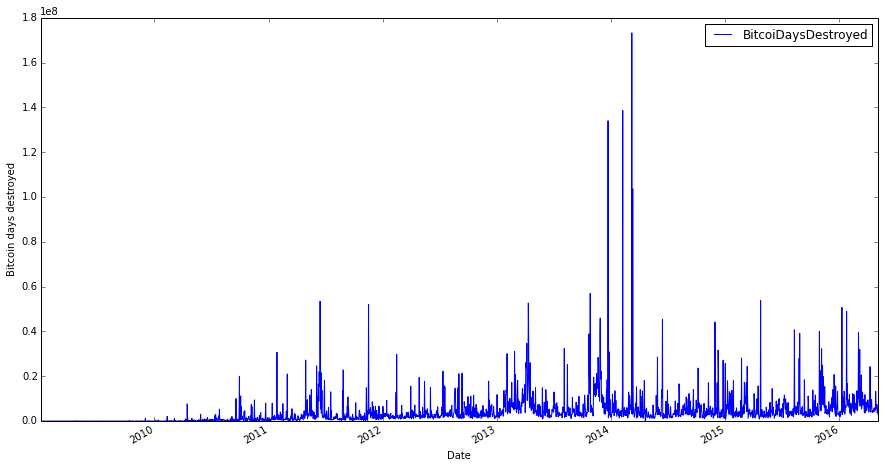
\includegraphics[width=1\linewidth]
    {gfx/bitcoin-days-destroyed-over-time}}
  \caption{\textit{Bitcoin days destroyed} chart}
  \label{fig:bitcoin-days-destroyed-over-time}
\end{figure}


% ----------------------------------------------------------------------

\section{Cost Per Transaction}
\label{sec:cost-per-transaction}

This variable shows miners revenue (in \textit{USD}) divided by the
number of transactions. Miners revenue are a result of the transaction
fees plus the reward for block discovery. The block discovery reward
is fixed by the community, and is up to the miner to accept any
transaction regardless of the fee in the transaction. A miner can
choose not to add any transaction at all to the block, or add
transactions with a $0$ \textit{BTC} fee.

\autoref{fig:cost-per-transaction-over-time} shows that in the end of
2010 the \textit{Cost per transactions} started to increase and had a
local maximum followed by another local maximum in mid 2011. This two
peaks took place in a low price of Bitcoin scenario, hence probably
the blocks were introduced with a small amount of transactions, and
with a subtle increase in the Bitcoin price the ratio would increase.

\begin{figure}[bth]
  \myfloatalign
  {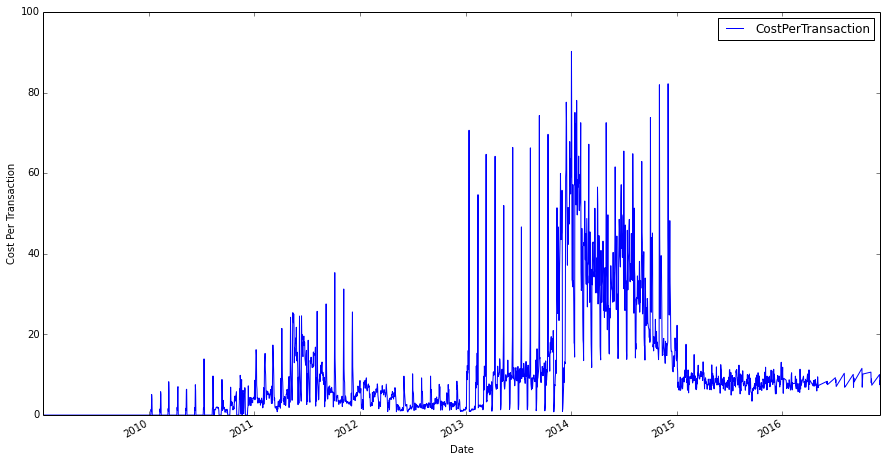
\includegraphics[width=1\linewidth]
    {gfx/cost-per-transaction-over-time}}
  \caption{\textit{Cost per transaction} chart}
  \label{fig:cost-per-transaction-over-time}
\end{figure}

On the contrary, the two peaks of 2014 are in the highest price of the
\textit{Bitcoin} history, where the number of transactions would make
little effect. Price in that period fluctuates between $700$
\textit{USD} and $1100$ \textit{USD} approximately.

\autoref{tab:cost-per-transaction} shows us that the median revenue is
$6.199964$ \textit{USD} and the mean is $9.731184$ \textit{USD}. This
information is later increased in
\autoref{sec:cost-per-transaction-percent}.

\begin{table}[bth]
  \caption{Statistical values for \textit{Cost per transaction}}
  \myfloatalign
  \tiny
  \begin{tabularx}{\textwidth}{XX} 
    \toprule
    \tableheadline{Measure} & \tableheadline{Value} \\
    \midrule
    count  & $2673$      \\
    mean   & $9.731184$  \\
    std    & $13.280920$ \\
    min    & $0$         \\
    $25\%$ & $1.295504$  \\
    $50\%$ & $6.199964$  \\
    $75\%$ & $10.413847$ \\
    max    & $90.202095$ \\
    \bottomrule
  \end{tabularx}
  \label{tab:cost-per-transaction}
\end{table}

%----------------------------------------------------------------------

\section{Cost Per Transaction Percent}
\label{sec:cost-per-transaction-percent}

This variable shows miners revenue as percentage of the transaction
volume. \autoref{fig:cost-per-transaction-percent-over-time} shows is
that the miners revenue has been near to zero all the time, excluding
few exceptions.

\begin{figure}[bth]
  \myfloatalign
  {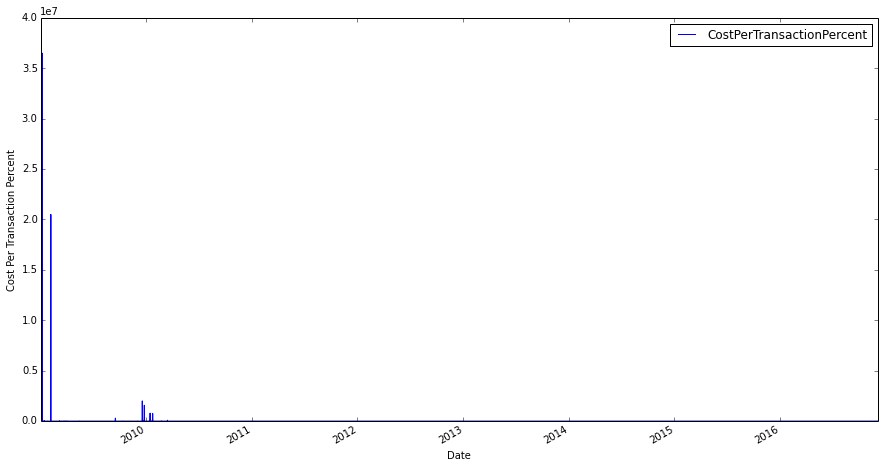
\includegraphics[width=1\linewidth]
    {gfx/cost-per-transaction-percent-over-time}}
  \caption{\textit{Cost per transaction percent} chart}
  \label{fig:cost-per-transaction-percent-over-time}
\end{figure}

As of 2016, miners are more concerned about the reward obtained by
discovering new blocks in the \textit{Bitcoin} network. In the future
the median percentage is $3.297002$ (see
\autoref{tab:cost-per-transaction-percent}) will probably increase,
because the sole income for miners will be transaction fees.

\begin{table}[bth]
  \caption{Statistical values for \textit{Cost per transaction percent}}
  \myfloatalign
  \tiny
  \begin{tabularx}{\textwidth}{XX} 
    \toprule
    \tableheadline{Measure} & \tableheadline{Value} \\
    \midrule
    count  & $2673$         \\
    mean   & $2.364769e+04$ \\
    std    & $8.113123e+05$ \\
    min    & $0$            \\
    $25\%$ & $1.583523$     \\
    $50\%$ & $3.297002$     \\
    $75\%$ & $9.613778$     \\
    max    & $3.65e+07$     \\
    \bottomrule
  \end{tabularx}
  \label{tab:cost-per-transaction-percent}
\end{table}

%----------------------------------------------------------------------

\section{Estimated Transaction Volume}
\label{sec:estimated-transaction-volume}


The total estimated value of transactions on the \textit{Bitcoin}
blockchain (does not include coins returned to sender as change). The
transaction volume represented in
\autoref{fig:estimated-transaction-volume-over-time} is very slowly
increasing, meaning that more transactions in \textit{Bitcoin} are
processed. However, it doesn't represent the actual value of
transactions, because people think in their local currency when
trading or shopping, and \textit{Bitcoin}'s value is volatile. The
next variable, \textit{Estimated Transaction Volume USD}, is more
appropriate for measuring the transactions volume as it gives us the
value of transactions in \textit{USD}. The peak that happened in 2012
wouldn't occur easily today due to the current value of
\textit{Bitcoin}.

\begin{figure}[bth]
  \myfloatalign
  {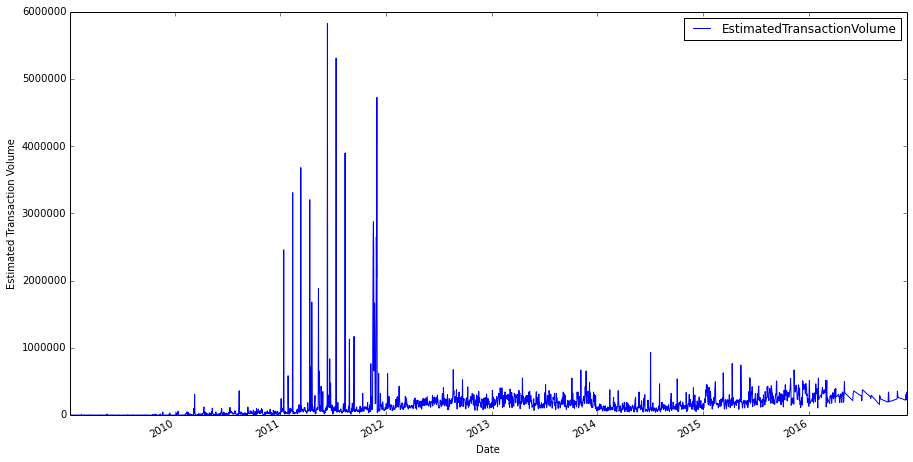
\includegraphics[width=1\linewidth]
    {gfx/estimated-transaction-volume-over-time}}
  \caption{\textit{Estimated transaction volume} chart}
  \label{fig:estimated-transaction-volume-over-time}
\end{figure}

%----------------------------------------------------------------------

% \section{Estimated Transaction Volume USD}
% \label{sec:estimated-transaction-volume-usd}


% The Estimated Transaction Volume in \textit{USD} value, shown in
% \autoref{fig:estimated-transaction-volume-usd-over-time}, can be
% explained by the average value of \textit{Bitcoin}, shown in
% \autoref{fig:market-price-over-time}, because nearly all the events
% are paired in the two figures. There is a small increase in estimated
% transaction volume in \textit{USD} in mid 2011 at the same time than the
% average price of \textit{Bitcoin} increases. Later on, in 2013 there is a
% bigger increase in estimated volume that is also reflected in the
% average price. Then we have the two biggest peaks around January of
% 2014 coinciding with the highest average value of \textit{Bitcoin} (also
% represented in two peaks). After that there is decrease in average
% price and estimated volume till 2016 where \textit{Bitcoin} average price
% starts to increase at the same time that the estimate transaction
% volume increases.

% \begin{figure}[bth]
%   \myfloatalign
%   {\includegraphics[width=1\linewidth]
%     {gfx/estimated-transaction-volume-usd-over-time}}
%   \caption{\textit{Estimated transaction volume \textit{USD}} chart}
%   \label{fig:estimated-transaction-volume-usd-over-time}
% \end{figure}

% %----------------------------------------------------------------------

\section{Difficulty}
\label{sec:difficulty}


This variable depicts a relative measure of how difficult it is to
find a new block. The \textit{Difficulty} is adjusted periodically as
a function of how much hashing power has been deployed by the network
of miners. \autoref{fig:difficulty-over-time} displays the difficulty
values over time. It can be noticed the staggered nature of the
values, that is because the \textit{Difficulty} is adjusted
automatically every 2016 blocks, and changes equally for the entire
\textit{Bitcoin} network. Until 2014, the difficulty of mining was
very low, it started to raise probably because the trade volume in the
end of 2013 and start of 2014 was approximately 70.000.000\$, which
attracted professional miners with a greater processing power, those
creating more and more blocks and augmenting the difficulty of mining.

\begin{figure}[bth]
  \myfloatalign
  {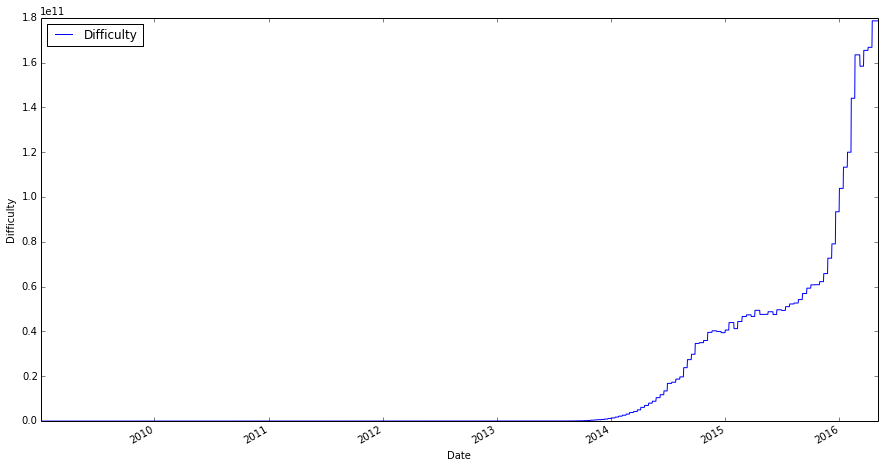
\includegraphics[width=1\linewidth]
    {gfx/difficulty-over-time}}
  \caption{\textit{Difficulty} chart}
  \label{fig:difficulty-over-time}
\end{figure}

%----------------------------------------------------------------------

\section{Euro price in USD}
\label{sec:euro-price-in-usd}


\textit{Euro price in USD} provided by the \textit{European Central
Bank (ECB)} is a variable that shows the \textit{Euro} price in
\textit{USD}. We have found latent values which have been interpolated
in order to fill them.

As shown in \autoref{fig:euro-price-in-usd-over-time} the value of
\textit{Euro} has been above that of the \textit{USD} from its
creation, been the period of 2000 through 2003 its closer price to
each other. From 2003 to 2007 the price of the \textit{Euro}
increased, coinciding with an increase on the interest imposed by the
\textit{ECB}. This increase in the interest of the credits is followed
by the collapse of the housing bubble in 2007, where the price of the
\textit{Euro} kept increasing, altough the interest was maintained by
the \textit{ECB} until 2009 where the \textit{ECB} started to lower
it. The increase in the \textit{Euro} price is probably due to
strategies of the \textit{Federal Reserve} to lower the price of the
\textit{USD}. Finally in 2015, the \textit{ECB} lowered the interests
of credits approaching the $0.0\%$, and that's reflected with a
decrease in the price of the \textit{Euro} with respect to
\textit{USD}.

\begin{figure}[bth]
  \myfloatalign
  {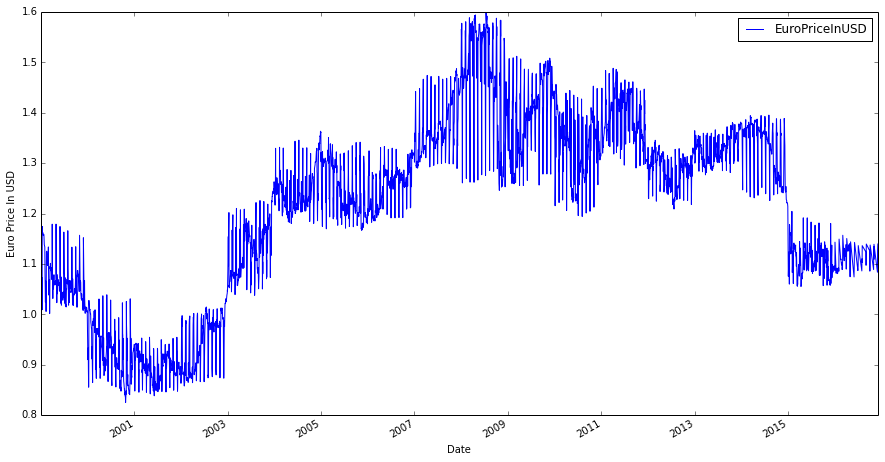
\includegraphics[width=1\linewidth]
    {gfx/euro-price-in-usd-over-time}} 
  \caption{\textit{Euro price in USD} chart}
  \label{fig:euro-price-in-usd-over-time}
\end{figure}

%----------------------------------------------------------------------

\section{Market Price}
\label{sec:market-price}



The \textit{USD} value of \textit{Bitcoin}, as calculated by the daily
average market price across major exchanges. This variable is related
to many others, starting with the number of transactions, that can
explain the fluctuations in the \textit{Bitcoin} price and different
events. In March 9, 2011, the \textit{Bitcoin} reaches parity with
\textit{USD} which is shown in a timid growth in market price followed
by a decrease (see \autoref{fig:market-price-over-time}).

\begin{figure}[bth]
  \myfloatalign
  {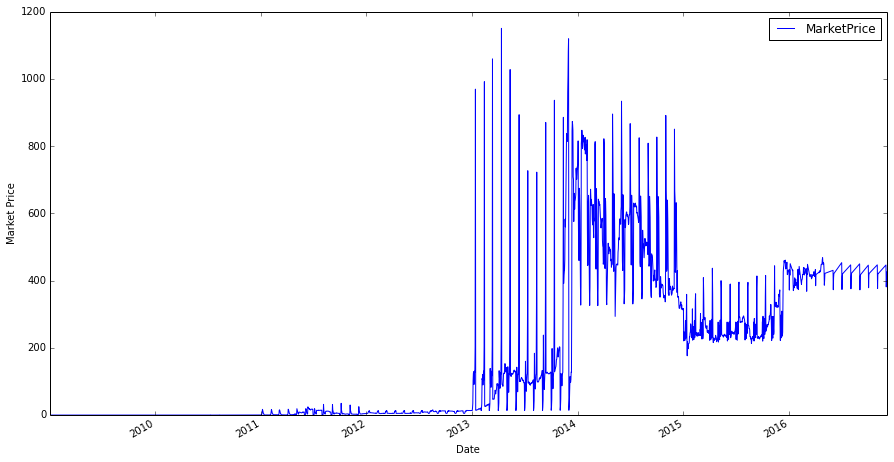
\includegraphics[width=1\linewidth]
    {gfx/market-price-over-time}}
  \caption{\textit{Market price} chart}
  \label{fig:market-price-over-time}
\end{figure}

After that there isn't a big growth until 2013, where several things
happen, Mega, the cloud storage service, starts accepting
\textit{Bitcoin}s, Internet Archive starts accepting
\textit{Bitcoin}s, a new food service
\href{PizzaForCoins.com}{PizzaForCoins.com} accepts \textit{Bitcoin}s
as a payment for food, CoinDesk is launched by Spotify investor and
Coinbase receives 5 million \textit{USD} in funding. This, and several
other events increase the market price of \textit{Bitcoin}.

After that there is a decrease in market price of \textit{Bitcoin},
maybe because MtGox, the largest exchange operator at the time, was
seized by The United States Department of Homeland Security.

In the second half of 2013, various events happen that can be the
cause of the raise of \textit{Bitcoin} market price, first, in August
6th, \textit{Bitcoin} is ruled currency by a Texas judge, then in
August 20th, \textit{Bitcoin} is ruled as private money in Germany,
then in August 28th, RoboCoin, a \textit{Bitcoin} ATM manufacturer,
starts accepting orders. This can be the cause of the huge peek at the
end of 2013 and start of 2014, where it reaches its highest value (see
\autoref{tab:market-price}). There are no clear events in the
\textit{Bitcoin} history that explain the period after 2014, which
leads us to think that the price has been fluctuating due to trading
strategies.

\begin{table}[bth]
  \caption{Statistical values for \textit{Market price}}
  \myfloatalign
  \tiny
  \begin{tabularx}{\textwidth}{XX} 
    \toprule
    \tableheadline{Measure} & \tableheadline{Value} \\
    \midrule
    count & $2673$ \\
    mean & $155.375541$ \\
    std & $218.398495$ \\
    min & $0$ \\
    $25\%$ & $0.199$ \\
    $50\%$ & $12.28$ \\
    $75\%$ & $270$ \\
    max & $1151$ \\
    \bottomrule
  \end{tabularx}
  \label{tab:market-price}
\end{table}

Is important to note how volatile is the \textit{Bitcoin} average
price, ranging from nearly $0$ \textit{USD} to $1151$ \textit{USD} in
just a year (see \autoref{tab:market-price}), and now, in 2016
fluctuating in a range bigger than $10$ \textit{USD} on average. These
fluctuations, if predicted, can be very profitable for the trader.

%----------------------------------------------------------------------

\section{Median Confirmation Time}
\label{sec:median-confirmation-time}

The median time for a transaction to be accepted into a mined block
and added to the public ledger (note: only includes transactions with
miner fees). Until the end of 2011, the confirmation time is
negligible. There is an important event that can be related to the
growth of the \textit{median confirmation time}, and that is the
largest \textit{Bitcoin} fee in a single transaction, in December 12,
171 \textit{Bitcoin}s was paids as fee in block 157235.

If we look at \autoref{fig:median-confirmation-time-over-time} there
is a peak in mid 2012, that can coincide with the increase in
\textit{output volume} seen in \autoref{fig:output-volume-over-time}.

\begin{figure}[bth]
  \myfloatalign
  {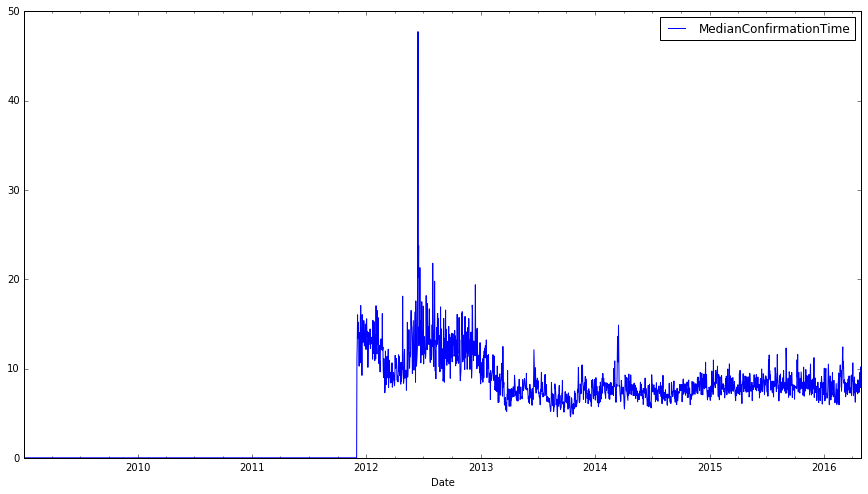
\includegraphics[width=1\linewidth]
    {gfx/median-confirmation-time-over-time}}
  \caption{\textit{Median confirmation time} chart}
  \label{fig:median-confirmation-time-over-time}
\end{figure}

% ----------------------------------------------------------------------

\section{Number of Transactions}
\label{sec:n-transactions-multiple}

Here we analyze \textit{number of transactions}, which is defined as
``\textit{The number of daily confirmed \textit{Bitcoin}
transactions}''. The \textit{number of transactions} represented in
\autoref{fig:n-transactions-over-time} show a moderated growth
compared to that of the market price. That may be because this
variable doesn't depend on the inflation of the \textit{Bitcoin}, and
there aren't exaggerated fluctuation. We see that even the price of the
\textit{Bitcoin} is not at its peak in 2016, the \textit{number of
transactions} are at its higher point so far in the \textit{Bitcoin}
history.

\begin{figure}[bth]
  \myfloatalign
  {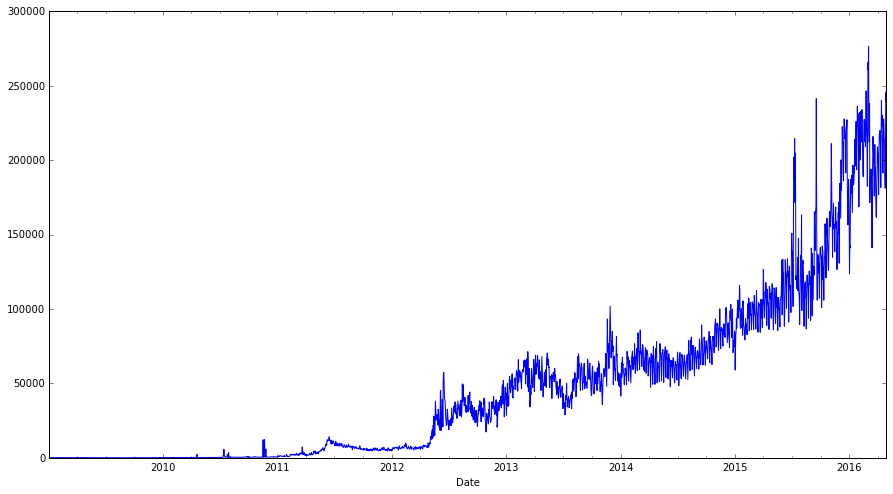
\includegraphics[width=1\linewidth]
    {gfx/n-transactions-over-time}}
  \caption{\textit{Number of transactions} chart}
  \label{fig:n-transactions-over-time}
\end{figure}

% ----------------------------------------------------------------------

\section{Output Volume}
\label{sec:output-volume}

The total value of all transaction outputs per day (includes coins
returned to the sender as change). There are a lot of events that
appear in \textit{output
volume}(\autoref{fig:output-volume-over-time}) that also appear in
\textit{market price}(\autoref{fig:market-price-over-time}) showing
that there is a strong relationship between the two measures.

\begin{figure}[bth]
  \myfloatalign
  {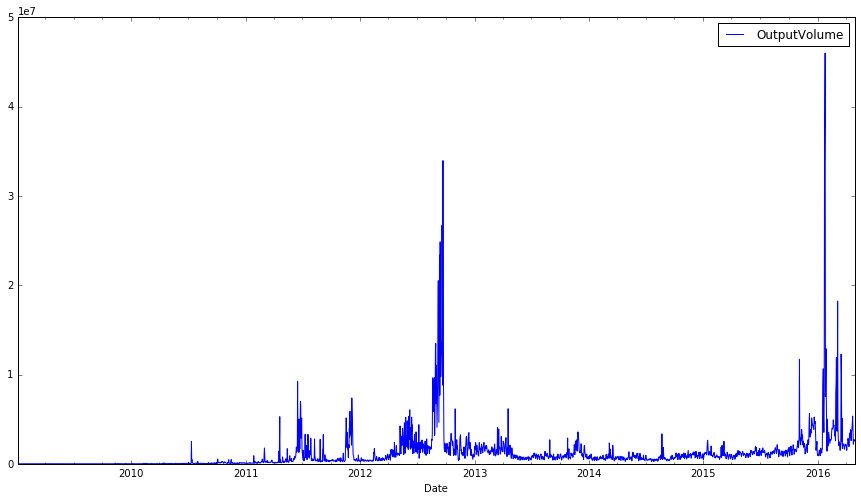
\includegraphics[width=1\linewidth]
    {gfx/output-volume-over-time}}
  \caption{\textit{Output volume} chart}
  \label{fig:output-volume-over-time}
\end{figure}

It's easier to understand the meaning of output and change returned to
the sender in the \textit{Bitcoin} world with an explanation given by
a user nicknamed \textit{DeathAndTaxes} in
\href{https://bitcointalk.org/index.php?topic=99593.0}{Bitcointalk.org}:

``\textit{\textit{Bitcoin} can only create transactions by using as
the input an ENTIRE prior unspent output. The most important thing to
realize is that \textit{Bitcoin} tx have inputs and outputs. The
"value" of your wallet is an abstraction. It is simply your client
(software which analyzes the wallet) taking a SUM of all the unspent
outputs which you have private keys for. The input of a tx is the
output of a PRIOR tx. You can only use unspent outputs in a new tx.
Once they are part of a tx they can never be used again ("spent").}

\textit{Say you I send you 50 BTC (for simplicity lets assume this is
compromised of a single 50 BTC output). No matter how you spend that
the input for the tx will be 50 BTC.}

\textit{Want to spend 20 BTC? Input: 50 BTC Output: 20 BTC + 30 BTC
"change" back to an address you control. Want to spend 1 BTC? Input:
50 BTC Output: 1 BTC + 49 BTC "change" back to an address you
control.}''

Output can be due to three circumstances, large amout of transactions,
transactions of big amount of \textit{Bitcoin}s, and big amount of
change returned to sender. The peak of 2013 is clearly due to change
received by sender as \textit{DeathAndTaxes} explains: ``\textit{In
the early days of \textit{Bitcoin} there really was nothing to "spend"
it on so most tx tended to be accumulation. This resulted in most
addresses having very large unspent outputs. As people started
"breaking" up those unspent outputs in tx involving smaller amounts
most of the volume WAS change.}''

%--------------------------------------------------------------------- 

\section{Standard \& Poors 500}
\label{sec:standard-and-poors-500}


From the
\href{https://en.wikipedia.org/wiki/S\%26P_500_Index}{Wikipedia}:

``\textit{The Standard \& Poor's 500, often abbreviated as the S\&P
500, or just "the S\&P", is an American stock market index based on
the market capitalizations of 500 large companies having common stock
listed on the NYSE or NASDAQ. The S\&P 500 index components and their
weightings are determined by S\&P Dow Jones Indices. It differs from
other U.S. stock market indices, such as the Dow Jones Industrial
Average or the Nasdaq Composite index, because of its diverse
constituency and weighting methodology. It is one of the most commonly
followed equity indices, and many consider it one of the best
representations of the U.S. stock market, and a bellwether for the
U.S. economy. The National Bureau of Economic Research has classified
common stocks as a leading indicator of business cycles.}''

We can see the description of certain events of
\autoref{fig:standard-and-poors-500-over-time} also from
\href{https://en.wikipedia.org/wiki/S\%26P_500_Index}{Wikipedia}:

\begin{figure}[bth]
  \myfloatalign
  {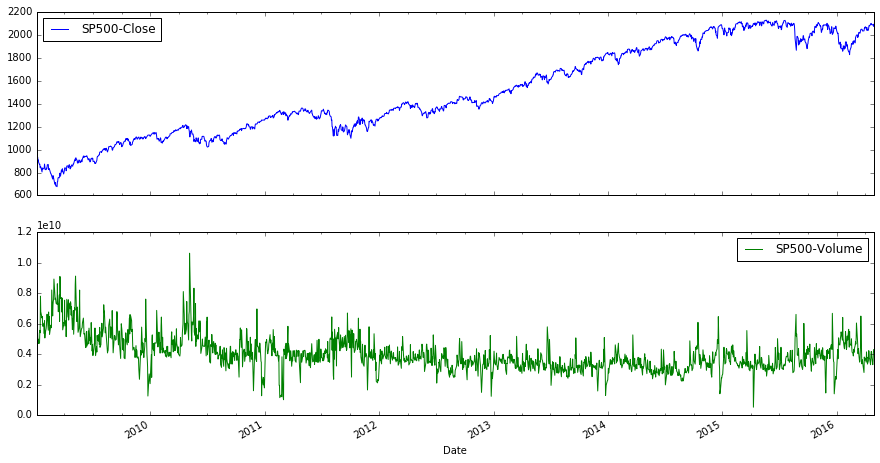
\includegraphics[width=1\linewidth]
    {gfx/standard-and-poors-500-over-time}}
  \caption{\textit{Standard \& poors 500}
    chart}
  \label{fig:standard-and-poors-500-over-time}
\end{figure}

``\textit{In mid-2007, the subprime mortgage crisis spread to the
wider U.S. financial sector. The resulting situation became acute in
September 2008, ushering in a period of unusual market volatility,
encompassing record 100-point swings in both directions and reaching
the highest levels since 1929. On November 20, 2008, the index closed
at 752.44, its lowest since early 1997. A modest recovery the
following day still left the index down 45.5\% for the year. This
year-to-date loss was the greatest since 1931, when the broad market
declined more than 50\%. The index closed the year at 903.25, for a
loss of 38.5\%. The market continued to decline in early 2009,
surrounding the financial crisis of 2008. The index reached a nearly
13-year low, closing at 676.53, on March 9, 2009.}

\textit{On March 23, 2009, the S\&P 500 marked a 20\% gain when it hit
822.92. The Dow Jones Industrial Average soon followed. The close for
2009 was 1,115.10, making it the second-best year of the decade. On
April 14, 2010 the index broke 1200 closing at 1210.65, but by July 2,
2010 it had closed at 1022.58. On April 29, 2011, the index closed at
1363.61, but it had a sharp drop in August and briefly broke 1100 in
October (with the VIX hitting 40). Gains continued despite significant
volatility amid electoral and fiscal uncertainty, and the 2012 close
of the S\&P 500 following QE3 was its third-highest ever, at 1,426.22
points. Many people hated the bull market. On March 28, 2013, it
closed above the closing high from 2007. On April 10, 2013, it also
closed above the intraday high from 2007.}

\textit{On May 3, 2013—more than 13 years since its first close above
1,500—the S\&P 500 closed above 1,600 for the first time, at 1,614.42.
This would be the first of three 100-point milestones in 2013: 1,600
on May 3, 2013; 1,700 on August 1, 2013; and 1,800 on November 22,
2013. The S\&P 500 closed out 2013 at a record high, finishing the
December 31, 2013, trading day at 1,848.36. On May 23, 2014, the index
for the first time closed above 1,900, at 1,900.53. On August 26,
2014, the index closed above 2,000 for the very first time, and on
December 22 the S\&P 500 climbed to 2078, an all-time high. The index
closed on December 29 at 2,090.57 with a closing of 2,058.90 at the
end of 2014. This was a gain of 85\% (in price return, and 105\% in
total return) for the five years 2010-2014. On February 17, 2015, the
index first closed above 2,100, closing at 2,100.34. On February 25,
2015 it reached 2,119.59 during mid-day, and on the following day it
closed at record high of 2,115.48. On May 21, 2015, the index closed
at 2,130.82, its high point for the year. At the close of 2015, the
index hit 2,043.94, down 0.73\% for the year.}''

Variable \textit{close} has a linear increasing trend which can
probably be explained because of the inflation, while the volume is a
random walk, following no apparent trend or seasonality. To complete
the information and better understand the graphics shown the reader
can analyze \autoref{tab:standard-and-poors-500}.

\begin{table}[bth]
  \caption{Statistical values for \textit{Standard \& poors 500}}
  \myfloatalign
  \tiny
  \begin{tabularx}{\textwidth}{XXX} 
    \toprule
    \tableheadline{Measure} & \tableheadline{SP500-Close}
    & \tableheadline{SP500-Volume} \\
    \midrule
    count  & $2673$        & $2673$    \\
    mean   & $1503.979515$ & $4.000942e+09$ \\
    std    & $395.164083$  & $1.122921e+09$ \\
    min    & $676.530029$  & $5.362e+08$    \\
    $25\%$ & $1178.339966$ & $3.299395e+09$ \\
    $50\%$ & $1406.290039$ & $3.78247e+09$  \\
    $75\%$ & $1898.293335$ & $4.50811e+09$  \\
    max    & $2130.820068$ & $1.061781e+10$ \\
    \bottomrule
  \end{tabularx}
  \label{tab:standard-and-poors-500}
\end{table}

% ---------------------------------------------------------------------

\section{Total Bitcoins}
\label{sec:total-bitcoins}

The total number of bitcoins that have already been mined; in other
words, the current supply of bitcoins on the network. First we have to
know that, according to the
\href{https://en.wikipedia.org/wiki/Bitcoin}{Wikipedia} ``The bitcoin
protocol specifies that the reward for adding a block will be halved
every 210000 blocks (approximately every four years). Eventually, the
reward will decrease to zero, and the limit of 21 million bitcoins
will be reached circa 2140; the record keeping will then be rewarded
by transaction fees solely.'' As shown in
\autoref{fig:total-bitcoins-over-time} the growth of bitcoin amount
will decrease every time the difficulty increases, with 21 million
been the upper limit. This change in difficulty depend on the blocks
discovered by miners.

\begin{figure}[bth]
  \myfloatalign
  {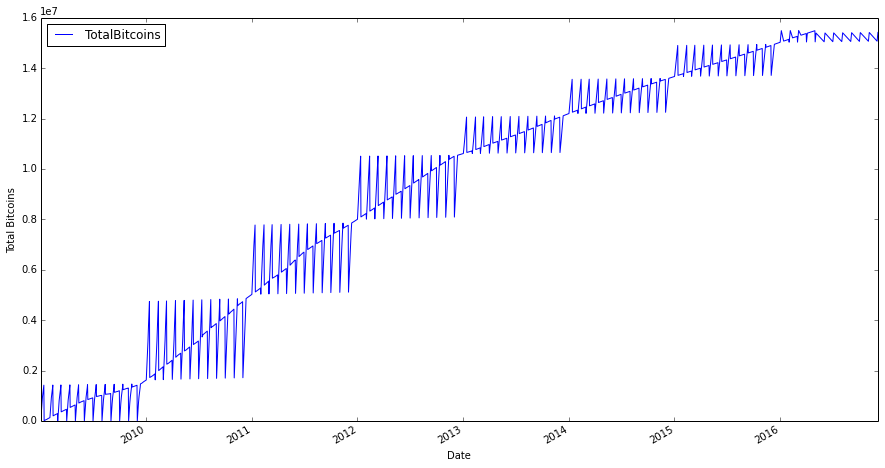
\includegraphics[width=1\linewidth]
    {gfx/total-bitcoins-over-time}}
  \caption{\textit{Total bitcoins} chart}
  \label{fig:total-bitcoins-over-time}
\end{figure}

%--------------------------------------------------------------------- 

\section{Trade Volume}
\label{sec:trade-volume}

The total \textit{USD} value of trading volume on major
\textit{Bitcoin} exchanges.

By comparing \textit{trade
volume}(\autoref{fig:trade-volume-over-time}) with other figures as
\textit{market price}(\autoref{fig:market-price-over-time}) it's clear
that there is a big bound between trade volume and market price of
\textit{Bitcoin}. There are peaks in mid 2011, March of 2013, December
of 2013, and the end of 2015 in both variable, showing the
aforementioned relationship.

\begin{figure}[bth]
  \myfloatalign
  {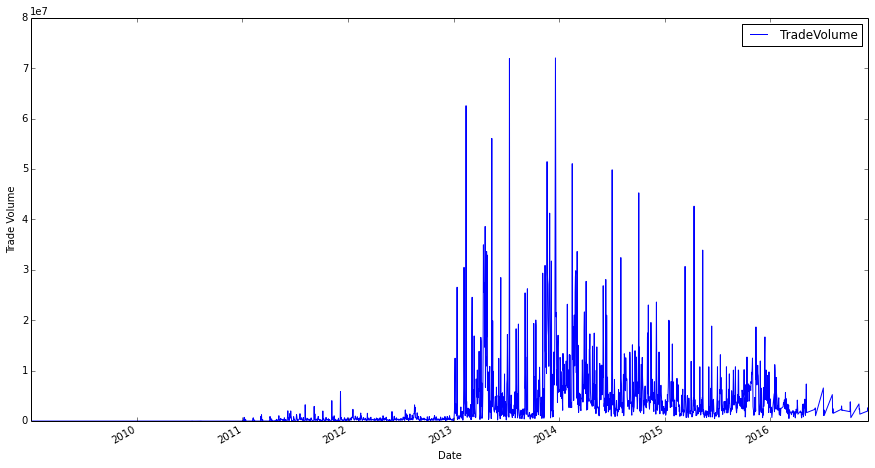
\includegraphics[width=1\linewidth]
    {gfx/trade-volume-over-time}}
  \caption{\textit{Trade volume}
    chart}
  \label{fig:trade-volume-over-time}
\end{figure}

Trade volume doesn't really exhibit the real activity in the
\textit{Bitcoin} network, because with this variable we don't see the
transactions between users. There is also another pattern that can be
seen in the trade volume, is that when the market price is maintained
the trade volume decreases, meaning that people are interested in the
\textit{Bitcoin} exchange when its price fluctuates.

%--------------------------------------------------------------------- 

\section{Transaction Fees}
\label{sec:transaction-fees}

The total value of all transaction fees paid to miners (not including
the coinbase value of block rewards) in \textit{BTC}. This variable
depends on the amount of transactions and the amount of fee paid per
transaction. If we look at \textit{transactions
fees}(\autoref{fig:transaction-fees-over-time}) we can see that even
there is an increase in the number of transactions near the peaks, the
height of those peaks is not comparable, in consequence we can assume
that at least those peaks are not due entirely to the number of
transactions made. We can see that there is some relationship with
\textit{market price}(\autoref{fig:market-price-over-time}),
reflecting how ``\textit{eager}'' is the user to have the transaction
accepted. This relationship is not in the sense that the peaks appear
simultaneously in the charts, but the peaks of \textit{transaction
fees} precede those of \textit{market price}. This can also be due to
the low price of \textit{Bitcoin} in those \textit{transaction fees}
peaks, because people think in \textit{USD} mostly, so they fix the
price of the fee in \textit{USD} instead of \textit{BTC} producing
those rises.

\begin{figure}[bth]
  \myfloatalign
  {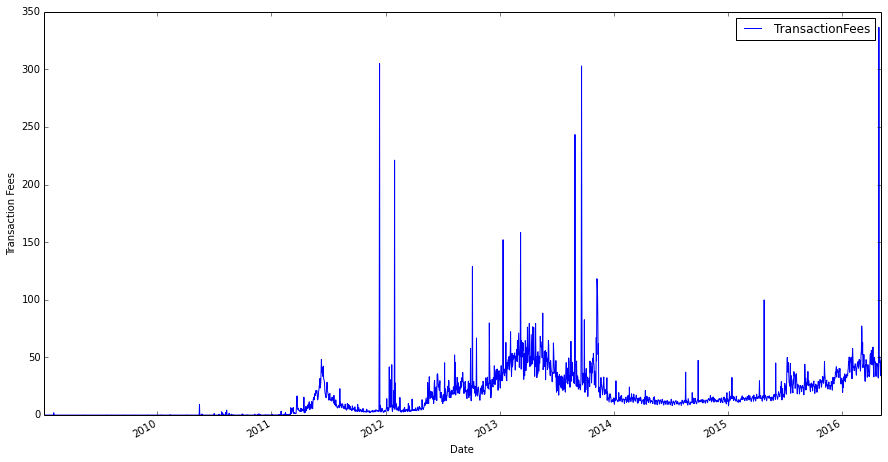
\includegraphics[width=1\linewidth]
    {gfx/transaction-fees-over-time}}
  \caption{\textit{Transaction Fees} chart}
  \label{fig:transaction-fees-over-time}
\end{figure}

%--------------------------------------------------------------------- 

\section{Transaction Fees USD}
\label{sec:transaction-fees-usd}

The total value of all transaction fees paid to miners (not including
the coinbase value of block rewards) in \textit{USD}.
\textit{Transaction fees usd}
(\autoref{fig:transaction-fees-usd-over-time}) shows how the fees
measured in \textit{USD} are more stable in time than fees measured in
BTC shown in \textit{transaction
fees}(\autoref{fig:transaction-fees-over-time}).

\begin{figure}[bth]
  \myfloatalign
  {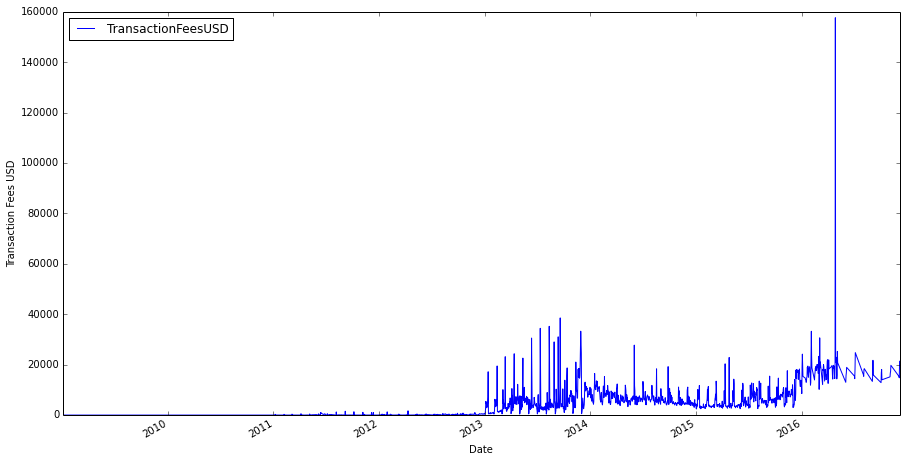
\includegraphics[width=1\linewidth]
    {gfx/transaction-fees-usd-over-time}}
  \caption{\textit{Transaction fees USD} chart}
  \label{fig:transaction-fees-usd-over-time}
\end{figure}

There highest fees prices have been paid in the last half of 2013 and
start of 2014, falling together with the highest price of
\textit{Bitcoin}, this can be explained because the users would want
their transactions to be processed before others. There is another
peak, very localized because it's only one day where the transactions
fees reach $157676.252$ \textit{USD} (see
\autoref{tab:transaction-fees-usd}), this can be because the
transactions/trade volume ratio is at its highest point since 2011,
which means that \textit{Bitcoin} transaction volume is even higher
than January of 2014 when the price of \textit{Bitcoin} was
approaching three times the current price, so we can assume that the
\textit{Bitcoin} transaction volume is due to number of transactions
more than amount of \textit{Bitcoin} per transaction.

\begin{table}[bth]
  \caption{Statistical values for \textit{Transaction fees USD}}
  \myfloatalign
  \tiny
  \begin{tabularx}{\textwidth}{XX} 
    \toprule
    \tableheadline{Measure} & \tableheadline{Value} \\
    \midrule
    count & $2673$ \\
    mean & $3476.856463$ \\
    std & $5990.380532$ \\
    min & $0$ \\
    $25\%$ & $0.001244$ \\
    $50\%$ & $273.841916$ \\
    $75\%$ & $5344.867164$ \\
    max & $157676.252853$ \\
    \bottomrule
  \end{tabularx}
  \label{tab:transaction-fees-usd}
\end{table}

%--------------------------------------------------------------------- 

\section{Transactions/Trade Ratio}
\label{sec:tx-trade-ratio}

\textit{transactions trade ratio}
(\autoref{fig:tx-trade-ratio-over-time}) presents the relationship
between \textit{BTC} transaction volume and \textit{USD} exchange
volume. This is another chart that can gives us an idea of the
transactions inside the \textit{Bitcoin} network, excluding the
trading.

\begin{figure}[bth]
  \myfloatalign
  {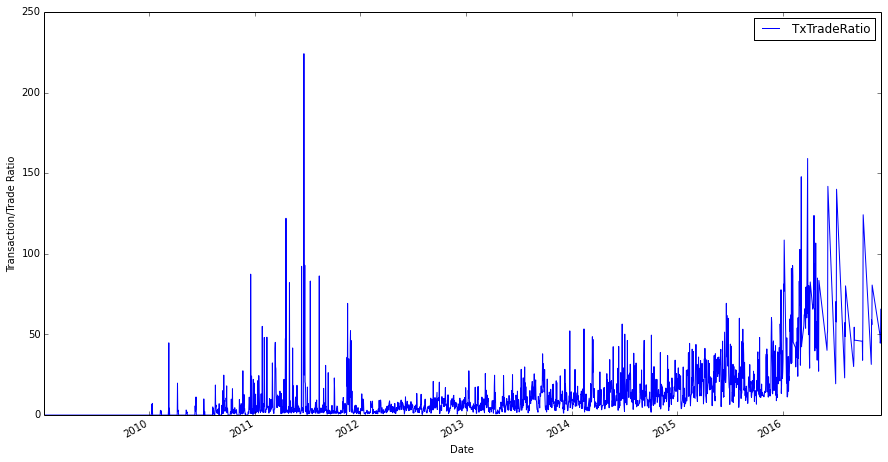
\includegraphics[width=1\linewidth]
    {gfx/tx-trade-ratio-over-time}}
  \caption{\textit{Transactions/trade ratio} chart}
  \label{fig:tx-trade-ratio-over-time}
\end{figure}

High values of this variable can mean two different things. One is
that the value of \textit{Bitcoin} is very low, as in 2011, and the
transactions between users, no matter how high they are, measured in
\textit{Bitcoin}, are going to have low values measured in
\textit{USD}. The other explanation is that there are a lot of
transactions inside the \textit{Bitcoin} network compared with the
\textit{USD} echange volume, even if the \textit{Bitcoin} price is
high, which would probably mean that there is a high usage of
\textit{Bitcoin} as a currency between individuals, this may be the
cause of the raise of this ratio since the end of 2015.

%--------------------------------------------------------------------- 

\section{Wikipedia Trend for Bitcoin}
\label{sec:wikipedia-trend-for-bitcoin}

The particular trend used in this case is the page views per day of
the \textit{Bitcoin} article in the English version of Wikipedia. The
daily visits to this paige has been as high as $923659$ (see
\autoref{tab:wikipedia-trend-for-bitcoin}), and a mean of
$8168.301160$.

\begin{table}[bth]
  \caption{Statistical values for \textit{Wikipedia trend for bitcoin}}
  \myfloatalign
  \tiny
  \begin{tabularx}{\textwidth}{XX} 
    \toprule
    \tableheadline{Measure} & \tableheadline{Value} \\
    \midrule
    count & $2673$ \\
    mean & $8168.301160$ \\
    std & $25977.892265$ \\
    min & $0$ \\
    $25\%$ & $86$ \\
    $50\%$ & $4173$ \\
    $75\%$ & $8585$ \\
    max & $923659$ \\
    \bottomrule
  \end{tabularx}
  \label{tab:wikipedia-trend-for-bitcoin}
\end{table}

For a better understanding of this variable we can rely on the
ubiquitous \textit{market price} since \textit{Bitcoin}s allure is
it's price and fluctuation with respect to more stable currencies like
\textit{USD} or \textit{EUR}. There are a number of events that can
produce the spike produced in second half of 2015 (see
\autoref{fig:wikipedia-trend-for-bitcoin-over-time}).

\begin{figure}[bth]
  \myfloatalign
  {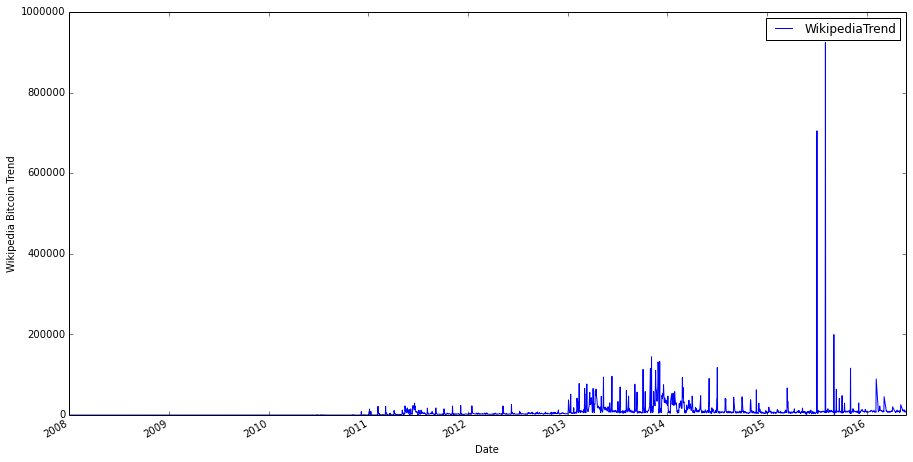
\includegraphics[width=1\linewidth]
    {gfx/wikipedia-trend-for-bitcoin-over-time}}
  \caption{\textit{Wikipedia trend for bitcoin}
    chart}
  \label{fig:wikipedia-trend-for-bitcoin-over-time}
\end{figure}

In January the \textit{New York Stock Exchange} invests $75M$
\textit{USD} in Coinbase. In March the results of the \textit{UK
Treasury}'s call for information on digital currency are announced. In
May the 19th Ross Ulbricht, operator of the \textit{Silk Road}
marketplace, is sentenced to life in prison. In June the 3rd, New York
state releases the BitLicense, a set of customized rules meant to
regulate \textit{Bitcoin} and digital currency businesses that serve
customers located in New York state. In July the 1st, two federal
agents plead guilty to \textit{Silk Road} theft during their active
investigation of the marketplace. In August the 1st, Mark Karpeles,
the CEO of the failed \textit{Bitcoin} exchange Mt. Gox, was arrested
in Japan on charges of fraud and embezzlement in relation to collapse
of the exchange. \textit{Bitcoin} Core developers Mike Hearn and Gavin
Andresen released a separate version of the \textit{Bitcoin} client
software, called \textit{Bitcoin XT}. The release illustrates an
ongoing controversy in the \textit{Bitcoin} development community:
\textit{What limit should be placed on the size of \textit{Bitcoin}'s
blocks?}. In October the 22nd, The \textit{European Court of Justice}
ruled that the exchange of \textit{Bitcoin} and "virtual currencies"
is not subject to \textit{value added tax (VAT)} in the
\textit{European Union}. In October, the 31st, \textit{Bitcoin} is
featured on front page of The Economist. In November, the 3rd,
\textit{Bitcoin} sign is accepted into Unicode. This are all events
that may have produced many visits to the \textit{Bitcoin} Wikipedia
page.

%--------------------------------------------------------------------- 

\chapter{Feature subset selection}
\label{ch:feature-selection}

The process of \textit{feature subset selection (FSS)} used in this
thesis is composed of two steps. One where we choose a set of
variables with \textit{principal component analysis (PCA)}
(\cite{pearson1901liii}) which is going to be our feature super-set
for all the models. Later on, for selecting per-model subsets a
\textit{wrapper FSS (WFSS)} technique (\cite{kohavi1997wrappers}) is
used.

This approach to \textit{FSS} has been taken because wrapper methods
select an optimum (that can be local) set of features
(\cite{inza2004filter, kumari2011filter}) and, at the same time, they
are more computationally expensive than filter methods. We came out
with the mixed approach of selecting a super-set with \textit{PCA},
which is computationally cheap and then we selected the final subsets
with a wrapper method.

\textit{WFSS} is a greedy algorithm, also called a forward feature
selection. In each iteration a model is produced with a subset which
initially is composed of one variable. In each iteration of the
algorithm the variable that minimizes the error produced is added to
selected features. If in a iteration a variable selected doesn't
minimize the error of the selected features the algorithm has
finished.

The features presented in \autoref{ch:stat-var-analysis} where
obtained by running a \textit{PCA} over 41 variables selecting the 18
that added more information to the prediction.

We can see in \autoref{fig:explained-variance} an ordered
representation of the \textit{explained variance} of the dimensions
obtained by performing \textit{PCA} over the original data-set. This
information is what led us to choose 17 as the dimensions that has
some meaningful information to predict the \textit{Bitcoin} price.

\begin{figure}[bth]
  \myfloatalign
  {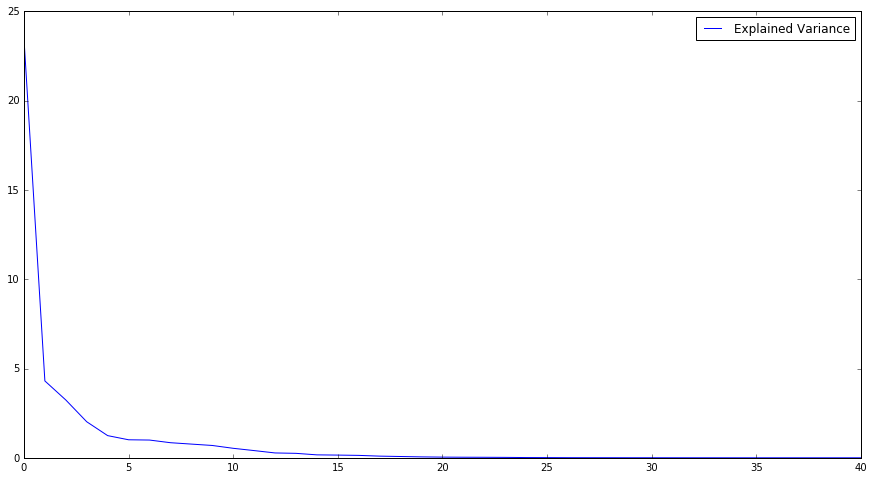
\includegraphics[width=1\linewidth]
    {gfx/explained-variance}}
  \caption{\textit{Explained variance} of PCA dimensions.}
  \label{fig:explained-variance}
\end{figure}

The results of \textit{WFSS} and the parameters used are explained in
\autoref{ch:experimental-setup}.

%\enlargethispage{2cm}

%------------------------------------------------

%%% Local Variables:
%%% mode: latex
%%% TeX-master: "../main"
%%% End:


\part{Methods \& Techniques}
% Method-Technique

\chapter{Introduction}
\label{ch:introduction}

\chapter{Vector Autoregression}
\label{ch:vector-autoregression}

\textit{Vector autoregressive models (VAR)} is a multivariate
prediction technique where in order to predict a value for each
variable is necessary to take into account the past values of the
variable and of other variables involved in the model. In \textit{VAR}
all variables are interdependent, which means that all variables
depend on the other variables involved in the multivariate system.
This interdependent systems are known in econometric as
\textit{endogenous}.

\textit{VAR} is a generalization of \textit{Autoregressive Models
  (AR)} applied to a vector of time series. Lets analyze the
mathematical expression of a \textit{first order VAR}, or simply
\textit{VAR(1)} for a bivariate system defined in \autoref{eq:var}.

\begin{equation}
  \begin{aligned}
    \label{eq:var}
    y_{1,t} & = c_1 + \phi_{11,1} y_{1,t-1} + \phi_{12,1} y_{2,t-1} +
    e_{1,t} \\
    y_{2,t} & = c_2 + \phi_{21,1} y_{1,t-1} + \phi_{22,1} y_{2,t-1} +
    e_{2,t} 
  \end{aligned}
\end{equation}

In this particular example $y_{i, t}$ describes the variable $i$ in
the temporal instant $t$. This equations define the relationship
between the two variables involved. As the name suggests
\textit{VAR(1)} takes into account only the first lag of each
variable, where $c_i$ is a constant offset and $\phi_{ij,l}$ is the
influence of variable $y_j$ on variable $y_j$ in the $l$-th lag.

\textit{VAR} models need two parameters for fitting. One is the number
of variables, denoted by $K$, and the other one is the number of lags
or $p$. The number of parameters to be estimated in a \textit{VAR} is
$K + p K^2$ or $1 + p K$ per equation. For \autoref{eq:var} there are
two variables, i.e. $K=2$, and only the first lag is used, i.e. $p=1$,
that makes a total of parameters to be estimated of
$2 + 1 \times 2^2 = 6$.

The generalized \textit{VAR(p)} expression would be
\autoref{eq:var-generalized}.

\begin{equation}
  \begin{aligned}
    \label{eq:var-generalized}
    \mathbf{y_t} = \mathbf{c} + \displaystyle\sum_{i=1}^p
    \pmb{\phi_i} \mathbf{y_{t-i}} + \pmb{\epsilon_t}
  \end{aligned}
\end{equation}

If the time series is stationary, we can predict their values by
directly fitting a \textit{VAR} to the data. On the other hand, if the
series is non-stationary we take differences to transform the time
series into a stationary one, and then, fit a \textit{VAR} to the
differenciated data. In both cases the model parameters are estimated
by \textit{OLS} per equation.

The predictions are generated recursively. \textit{VAR} generates a
prediction for each one of the variables involved in the model. Lets
take the \textit{VAR(1)} described in \autoref{eq:var}. \textit{VAR}
would estimate the parameters $\phi_{ij,l}$ and $c_i$ for $y_{i,t}$
such that $i \in \{1,2\}$ and $t = T$. Once the parameters has been
estimated by \textit{OLS} is possible to create the prediction
equations. \autoref{eq:var-prediction-1} describes the prediction
equation for $h=1$

\begin{equation}
  \begin{aligned}
    \label{eq:var-prediction-1}
    \hat{y}_{1,T+1|T} & = \hat{c}_1 + \hat{\phi}_{11,1} y_{1,T} +
    \hat{\phi}_{12,1} y_{2,T} \\ 
    \hat{y}_{2,T+1|T} & = \hat{c}_2 + \hat{\phi}_{21,1} y_{1,T} +
    \hat{\phi}_{22,1} y_{2,T}
  \end{aligned}
\end{equation}

\autoref{eq:var-prediction-1} is very similar to \autoref{eq:var}
except that the parameters has been replaced by its estimated values
and the error has been replaced by zero.

If the horizon we want to use is $h = 2$, the equation would be
\autoref{eq:var-prediction-2} where the values for past values of the
variable are replaced by predictions of those values.

\begin{equation}
  \begin{aligned}
    \label{eq:var-prediction-2}
    \hat{y}_{1,T+2|T} & = \hat{c}_1 + \hat{\phi}_{11,1} \hat{y}_{1,T+1} +
    \hat{\phi}_{12,1} \hat{y}_{2,T+1} \\ 
    \hat{y}_{2,T+2|T} & = \hat{c}_2 + \hat{\phi}_{21,1} \hat{y}_{1,T+1} +
    \hat{\phi}_{22,1} \hat{y}_{2,T+1}
  \end{aligned}
\end{equation}
\chapter{Recurrent Neural Networks}
\label{ch:recurrent-neural-networks}

\section{Artificial Neural Networks}

\textit{Artificial neural networks} are a learning model based on the
human brain's neural network structure. It represents graphically an
ideal structure that resembles that of the neuron and it's connections
with another neurons.

A simple \textit{ANN (artificial neural network)} can be seen in
\autoref{fig:one-layer-ann}. We can see in the first layer, called
\textit{input layer}, the nodes that represent the inputs, represented
as $x_0, x_1, x_2,$ and $x_3$, where $x_1$ through $x_3$ are actual
inputs, and $x_0$ is a \textit{bias term}. This \textit{bias term} is
always equal to 1.

Next we have the directed edges, which represent how the information
flow goes, in this case, the information flows from $x_0, x_1, x_2,
x_3$ to $a_1^{(2)}$, which is in the second layer. In other words,
$a_1^{(2)}$ has $x_0, x_1, x_2, x_3$ as inputs. This edges has
associated weights, which multiply the output of the origin node and
their purpose. In this particular network the weights are represented
by $W_0, W_1, W_2$ and $W_3$. The term $a_1^{(2)}$ means the first
neuron in the second layer. In the next layer, called \textit{output
layer}, we have the output neuron represented by $a_0^{(2)},$
mentioned before. The nodes in this layer have an \textit{activation
function} which can perform different computations with the inputs and
a matrix of weights $W$. In this case is the \textit{sigmoid function}
represented by $\sigma$ with the expression in
\autoref{eq:sigmoid-function}. The expression $h_W(x)$ means that the
output is a parameterized function of the inputs $x$ and that the
parameters are the components of the \textit{weight} matrix $W$.

\begin{figure}[bth]
  \myfloatalign
  {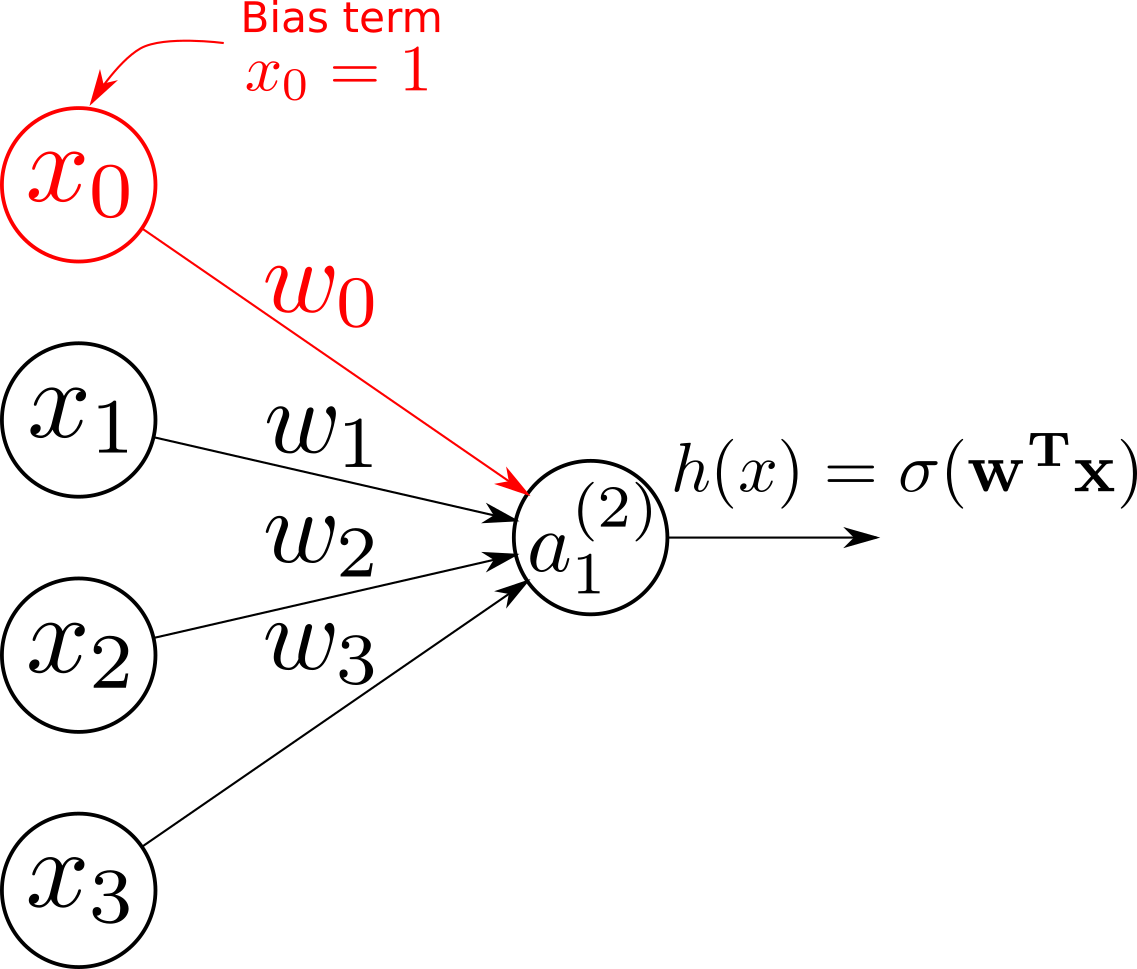
\includegraphics[width=.6\linewidth]
    {gfx/simple-ann-model}}
  \caption{One layer artificial neural network}
  \label{fig:one-layer-ann}
\end{figure}

As you can imagine, the network can have different topologies,
multiple hidden layers, different connection architectures, and
different activation functions. Let's take a look at a two layer
network in \autoref{fig:two-layer-ann}. Just as in
\autoref{fig:one-layer-ann} the first layer is the input layer, with
bias term $x_0$ and inputs $x_1, x_2$ and $x_3$. Next to the input
layer is the hidden layer, which also contains a bias term called
$a_0^{(2)}$ and hidden neurons called $a_1^{(2)}, a_2^{(2)}$ and
$a_3^{(2)}$. In this neural network architecture, called
\textit{multilayer perceptron (MLP)}, each layer is fully connected
with the next, therefore each neuron of the hidden layer except for
the bias term have all the neurons from the input layer as inputs.
Last we have the output layer, which contains a single neuron in
\textit{MLP} called $a_1^{(3)}$. This neuron gives the output of the
neural network which is $h_{W}(x)$.

\begin{figure}[bth]
  \myfloatalign
  {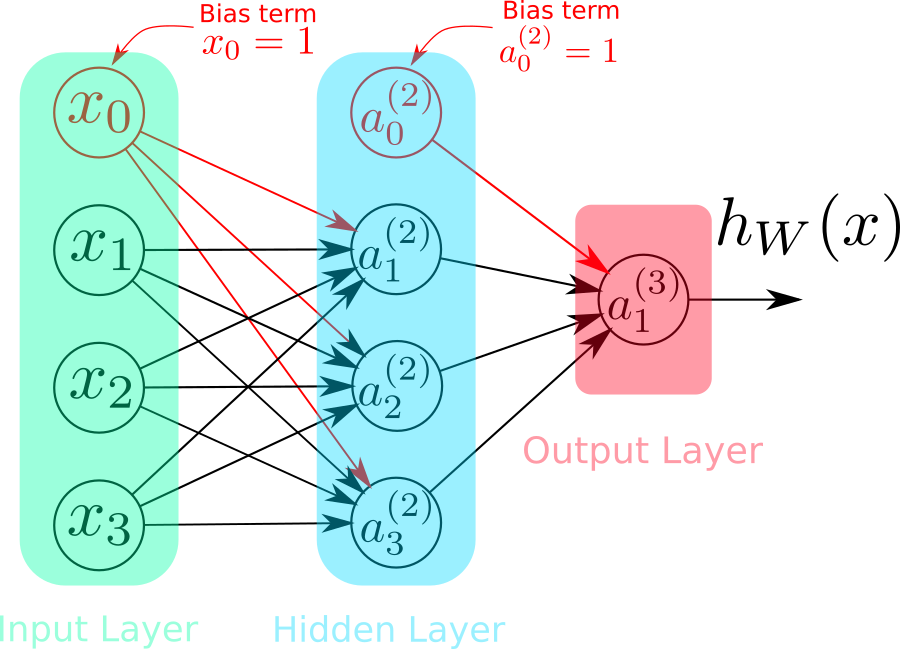
\includegraphics[width=1\linewidth]
    {gfx/two-layer-ann-model}}
  \caption{Two layer artificial neural network}
  \label{fig:two-layer-ann}
\end{figure}

Here we will try to write the relationship between input, output and
the parameters. Let's start by writing the mathematical expression of
the second layer in \autoref{eq:layer-2-expression}. Where
$W_{ik}^{(j)}$ is the weight controlling the mapping between layer $j$
and $j + 1$ for the $k$-th input of the $i$-th neuron in layer $j$,
and $\sigma$ is the activation function.

\begin{equation}
  \begin{aligned}
    \label{eq:layer-2-expression}
    a_1^{(2)} & = \sigma(W_{10}^{(1)} x_0 + W_{11}^{(1)} x_1
    + W_{12}^{(1)} x_2 + W_{13}^{(1)} x_3) \\
    a_2^{(2)} & = \sigma(W_{20}^{(1)} x_0 + W_{21}^{(1)} x_1
    + W_{22}^{(1)} x_2 + W_{23}^{(1)} x_3) \\
    a_3^{(2)} & = \sigma(W_{30}^{(1)} x_0 + W_{31}^{(1)} x_1
    + W_{32}^{(1)} x_2 + W_{33}^{(1)} x_3) \\
  \end{aligned}
\end{equation}

Following with the same procedure we can build the expression for the
output in \autoref{eq:output-expression}.

\begin{equation}
  \begin{aligned}
    \label{eq:output-expression}
    h_{W}(x) & = a_1^{(3)} = \sigma(W_{10}^{(2)} a_0^{(2)}
    + W_{11}^{(2)} a_1^{(2)} + W_{12}^{(2)} a_2^{(2)}
    + W_{13}^{(2)} a_3^{(2)} \\
  \end{aligned}
\end{equation}

We mentioned before the \textit{activation function}. This
\textit{activation function} takes the inputs of the neuron and
outputs a value to the next layer. This value can be a two state value
($\{0,1\}$), or a linear one. In classification the two-state value
are used, and for this outputs the expression that the
\textit{activation function} takes is frequently a \textit{sigmoid
function} or \textit{logistic function}, represented in
\autoref{eq:sigmoid-function}. We have been using a \textit{sigmoid
function} in all our \textit{activation functions}.

\begin{equation}
  \begin{aligned}
    \label{eq:sigmoid-function}
    \sigma(z) = \frac{1}{1 + e^{-z}}
  \end{aligned}
\end{equation}

\section{Backpropagation Algorithm}

\textit{BP} was developed in the context of control theory by
\cite{kelley1960gradient} and later applied to \textit{artificial
intelligence} by \cite{werbos1974beyond} and
\cite{rumelhart1988learning}.

We are going to use gradient descent to optimize the \textit{error
function} in terms of the \textit{weights} of the network. First we
need to find the gradient of the \textit{error function} in with
respect to the \textit{weights}, i.e. $\dfrac{\partial E}{\partial
  W_{ij}^{(l)}}$

In \autoref{eq:sigmoid-function-derivate} we calculate the derivative
of the \textit{sigmoid function} because we are going to use it all
over the \textit{backpropagation} explanation.

\begin{equation}
  \begin{aligned}
    \label{eq:sigmoid-function-derivate}
    \dfrac{d}{dz} \sigma(z) & = \dfrac{d}{dz} \frac{1}{1 + e^{-z}} =
    \dfrac{e^{-z}}{(1 + e^{-z})^2} = \dfrac{1 + e^{-z}}{(1 +
      e^{-z})^2} - \left( \dfrac{1}{1 + e^{-z}} \right)^2 \\
    & = \sigma(z) - (\sigma(z))^2 = \sigma(z)(1-\sigma(z))
  \end{aligned}
\end{equation}

Now let's define the \textit{error function} in
\autoref{eq:error-function}. Let's also define, for the purpose of
this explanation, three disjoint sets of neurons, i.e., the set of
neurons in the input layer which is called $I$ and is indexed by $i$
such as $ i \in I$, the set of neurons in a hidden layer which is
called $J$ and is indexed by $j$ such as $j \in J$, and the set of
neurons in the output layer called $K$ and is indexed by $k$ such as
$k \in K$.

\begin{equation}
  \begin{aligned}
    \label{eq:error-function}
    E = \frac{1}{2} \sum_{k \in K} (h_k - y_k)^2
  \end{aligned}
\end{equation}

To compute the gradient of the \textit{error function} we are going to
compute it for two of the three disjoint sets that we have established
before. Those sets are the \textit{output layer}, and the
\textit{hidden layer}. There's no need to compute the error for the
\textit{input layer} because there isn't an error associated with the
inputs.

In the calculation of the gradient of the output layer in
\autoref{eq:output-layer-error-function-gradient} we have $W_{jk}$
meaning a \textit{weight} between a neuron from the \textit{hidden
layer} to a neuron in the \textit{output layer}, $h_i$, $h_j$ and
$h_k$ are outputs of a neuron in the \textit{input layer},
\textit{hidden layer} or \textit{output layer} respectively.

\begin{equation}
  \begin{aligned}
    \label{eq:output-layer-error-function-gradient}
    \frac{\partial E}{\partial W_{jk}} & = \frac{\partial}{\partial
      W_{jk}} \frac{1}{2} \sum_{k \in K} (h_k - y_k)^2 \\
    & = (h_k - y_k)h_k(1-h_k)h_j \\
    \textbf{substitute } \delta_k & = (h_k - y_k)h_k(1-h_k) \implies \\
    & \implies \frac{\partial E}{\partial W_{jk}} = h_j \delta_k
  \end{aligned}
\end{equation}

Now for a hidden layer, the calculations of the gradient would be the
ones shown in \autoref{eq:hidden-layer-error-function-gradient}.

\begin{equation}
  \begin{aligned}
    \label{eq:hidden-layer-error-function-gradient}
    \frac{\partial E}{\partial W_{ij}} & = \frac{\partial}{\partial
      W_{ij}} \frac{1}{2} \sum_{k \in K} (h_k - y_k)^2 \\
    & = h_j(1-h_j)h_i \sum_{k \in K} (h_k - y_k) h_k(1 - h_k) W_{jk}  \\
    \textbf{substitute } \delta_k & = (h_k - y_k) h_k(1 - h_k) \implies \\
    & \implies \frac{\partial E}{\partial W_{ij}} = h_j(1-h_j)h_i
    \sum_{k \in K} \delta_k W_{jk} \\
    \textbf{substitute } \delta_j & = h_j(1-h_j) \sum_{k \in K} \delta_k
    W_{jk}  \implies \\ 
    & \implies \frac{\partial E}{\partial W_{ij}} = h_i\delta_j
  \end{aligned}
\end{equation}

Once we come up with the gradient results we can present the
backpropagation algorithm in \autoref{backpropagation-algorithm} to
obtain those gradients.

\begin{algorithm}[H]
  \caption{\textit{Backpropagation algorithm}}
  \label{backpropagation-algorithm}
  \begin{algorithmic}[1]
    \State Let the training set be $\{(x^{(1)},y^{(1)}),\dots,
    (x^{(m)},y^{(m)})\}$
    \State Set $\Delta_{ij}^{(l)} = 0$ for all $l,i,j$
    \For{ $i = 1$ to $m$ }
    \State Set $a^{(1)} = x^{(i)}$
    \State Propagate values to compute $a^{(l)}$ for $l = 2,
    3, \dots, L$
    \State Using $y^{(i)}$ compute $\delta^{(L)} = a^{(L)} - y^{(i)}$
    \State Compute $\delta^{(L-1)}, \delta^{(L-2)}, \dots,
    \delta^{(2)}$
    \State $\Delta_{ij}^{(l)} := \Delta_{ij}^{(l)} + a_j^{(l)} \delta_i^{(l+1)}$
    \EndFor
    \State $D_{ij}^{(l)} := \frac{1}{m} \Delta_{ij}^{(l)} + \lambda
    W_{ij}^{(l)}$ if $j \neq 0$
    \State $D_{ij}^{(l)} := \frac{1}{m} \Delta_{ij}^{(l)}$ if $j = 0$
  \end{algorithmic}
\end{algorithm}

In the forward pass, \textit{backpropagation} computes the values of
each neuron until getting the outputs, and in the backward pass,
\textit{backpropagation} computes the error gradients and updates the
\textit{weights} and \textit{biases} of the network.

\section{Recurrent Neural Network}
\label{sec:rnn-nets}

The general idea behind \textit{recurrent neural networks} is the
ability to use information from other elements of a sequence. Thus,
the input of RNNs are considered sequences. Whether they are time
sequences, or notes from a musical composition or words in a sentence,
RNNs can take advantage of this sequential nature of the input.

A \textit{recurrent neural network} (\cite{rumelhart1986sequential})
is a class of artificial neural network where connections between
units form a directed cycle as shown in \autoref{fig:rnn-structure}.
This creates an internal state of the network which allows it to
exhibit dynamic temporal behavior. Unlike feedforward neural networks,
RNNs can use their internal memory to process arbitrary sequences of
inputs. This makes them applicable to tasks such as unsegmented
connected handwriting recognition or speech recognition.

\begin{figure}[bth]
  \centering
  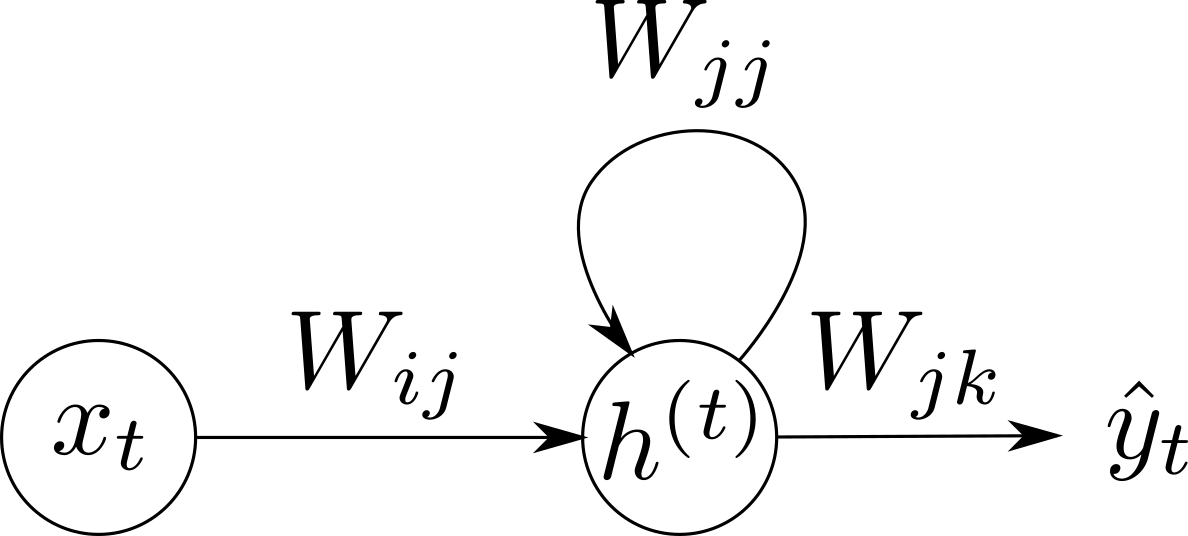
\includegraphics[width=.5\linewidth]{gfx/rnn.png}
  \caption{Recurrent Neural Network}
  \label{fig:rnn-structure}
\end{figure}

The two equations that govern the behavior of this type of neural nets
are described in \autoref{eq:rnn-equations}. This equation

\begin{align}
  \begin{split}
    \label{eq:rnn-equations}
    h^{(t)} & = \sigma(W_{ij} x^{(t)} + W_{jj} h^{(t-1)} + b_h ) \\
    \hat{y}^{(t)} & = \sigma(W_{jk} h^{(t)} + b_y ) \\
    W_{ij} & \gets \text{Matrix of weights between inputs and hidden
      layer} \\
    W_{jj} & \gets \text{Matrix of recurrent weights between hidden
      layer and itself} \\
    b_h, b_y & \gets \text{Biases to learn offsets}
  \end{split}
\end{align}

\section{Backpropagation through time}
\label{sec:bp-through-time}

\textit{Backpropagation through time (BPTT)}, introduced by
\cite{werbos1990backpropagation} is the use of
\textit{backpropagation} over an \textit{RNN}. To be able to apply
\textit{BPTT} there are some issues that must be taken into account.

First the \textit{RNN} need to be unfolded through time in a
\textit{feed forward network (FFN)}. This is done by creating a finite
set of new nodes that represent the same neuron in successive time
steps. This step is performed for every neuron in a \textit{hidden
layer}. This is done because \textit{backpropagation} can't be run
over a network with cycles. \autoref{fig:bptt-unfolded-rnn} shows the
3-step unfolded version of the \textit{RNN} shown in
\autoref{fig:rnn-structure}.

\begin{figure}[bth]
  \centering
  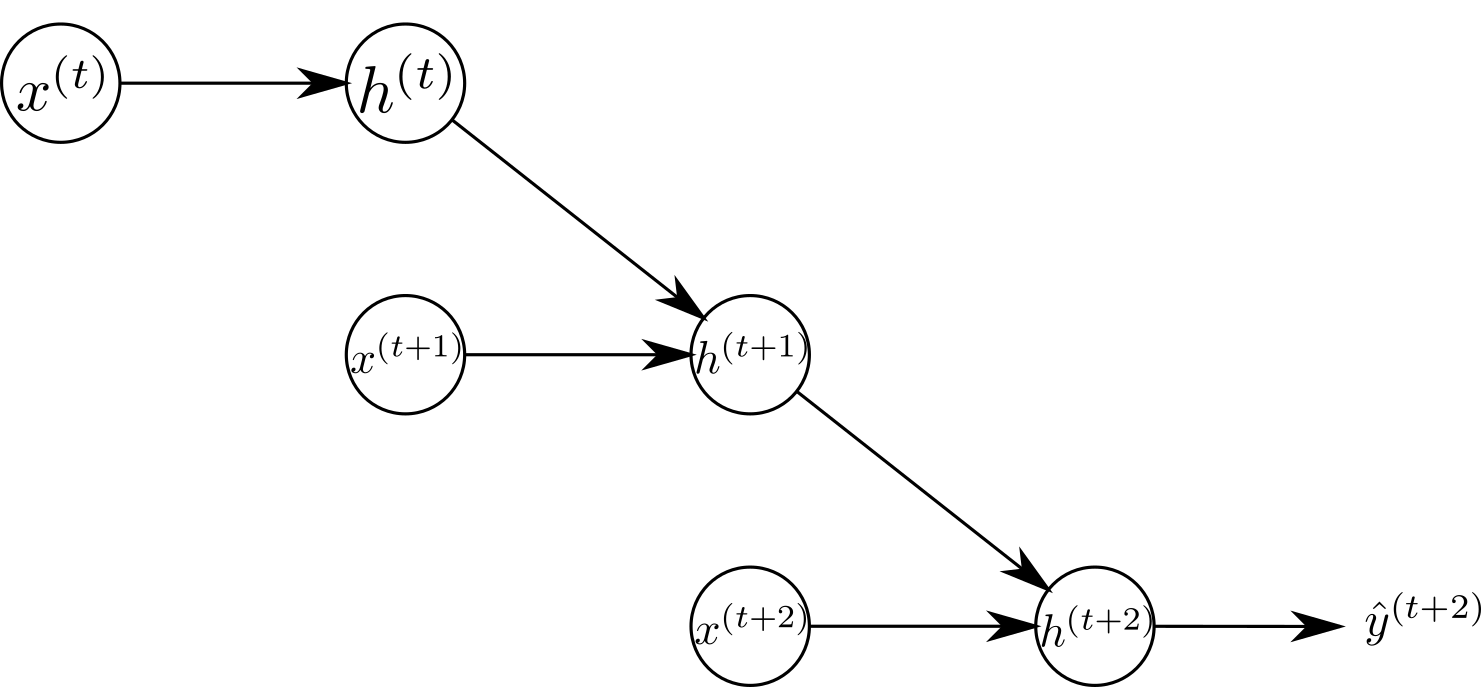
\includegraphics[width=.95\linewidth]{gfx/bptt-unfolded-rnn}
  \caption{Unfolded RNN for BPTT}
  \label{fig:bptt-unfolded-rnn}
\end{figure}

Second, as a consequence of the unfolding, we need to reproduce the
edges connecting those new nodes, so we establish a restriction by
which a set of edges in the \textit{FFN} that are reproduced from one
single edge in the \textit{RNN} need to update their weights by the
same amount. This can be enforced by averaging $\Delta W$ over all the
set each time is computed.
\autoref{fig:bptt-unfolded-rnn-weight-restrictions} shows the weight
restriction that would apply to the unfolded \textit{RNN} of
\autoref{fig:bptt-unfolded-rnn}.

\begin{figure}[bth]
  \centering
  \includegraphics[width=.95\linewidth]
  {gfx/bptt-unfolded-rnn-weight-restrictions}
  \caption{Weight restrictions in unfolded RNN}
  \label{fig:bptt-unfolded-rnn-weight-restrictions}
\end{figure}

%---------------------------------------------------------------------
%---------------------------------------------------------------------
%---------------------------------------------------------------------

%\enlargethispage{2cm}

%------------------------------------------------

%%% Local Variables:
%%% mode: latex
%%% TeX-master: "../main"
%%% End:


\part{Implementation}
% State Of The Art

\chapter{Implementation} % Chapter title

\label{ch:implementation}

%----------------------------------------------------------------------

\section{Statistical variable analysis}
\label{sec:stat-var-analysis}

This section describes the basic properties of each feature we are
using in this particular thesis. Among them we have the count of all
variables, mean, standard deviation, min value, max value, quartiles.
We also add the histogram to have an idea of how the distribution of
the variable works and the boxplot that can help us determine if there
are outliers in the data-set.

\subsection{Average Block Size}
\label{sec:avg-block-size}

A concise definition of a block can be found
\href{https://en.bitcoin.it/wiki/Block}{here}: \textit{``Each block
  contains, among other things, a record of some or all recent
  transactions, and a reference to the block that came immediately
  before it. It also contains an answer to a difficult-to-solve
  mathematical puzzle - the answer to which is unique to each
  block.''}

It's clear that, over time, the size of the block is going to
increase, because there are more and more transactions in the Bitcoin
distributed network, due to that
\autoref{fig:avg-block-size-over-time} shows a non-stoppable
increasing.

This variable, called avg-block-size represent the average size of the
blocks in one day measured in MB. One real number data point each day,
at 18:15:05, spanning from 03/01/2009 to 03/05/2016. It was obtained
from the section \textbf{Charts} of
\href{blockchain.info}{blockchain.info}

\begin{figure}[bth]
  \myfloatalign
  {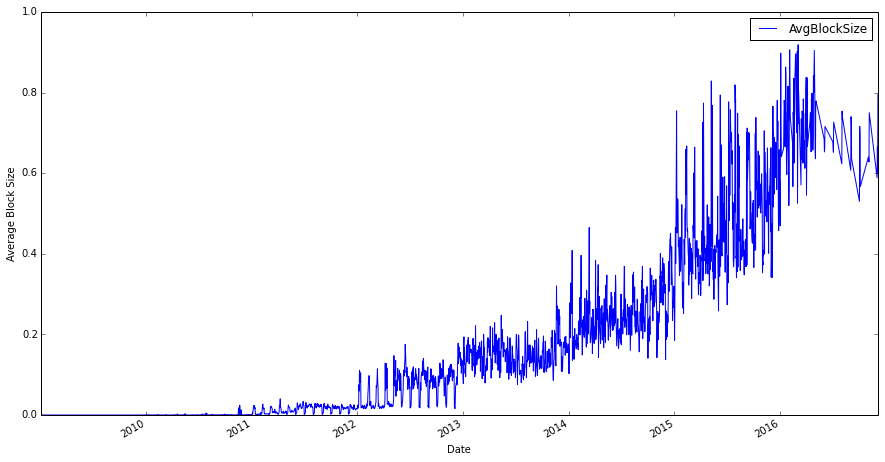
\includegraphics[width=1\linewidth]
    {gfx/avg-block-size-over-time}} 
  \caption{Average Block Size Over Time}
  \label{fig:avg-block-size-over-time}
\end{figure}

In \autoref{fig:avg-block-size-over-time} can be seen how the average
block size has been increasing since the creation of Bitcoin. In 2015
the average block started to dangerously approach the limit of 1 MB,
which is causing a big debate in the Bitcoin community whether they
should increase this limit or not.

\begin{figure}[bth]
  \myfloatalign
  {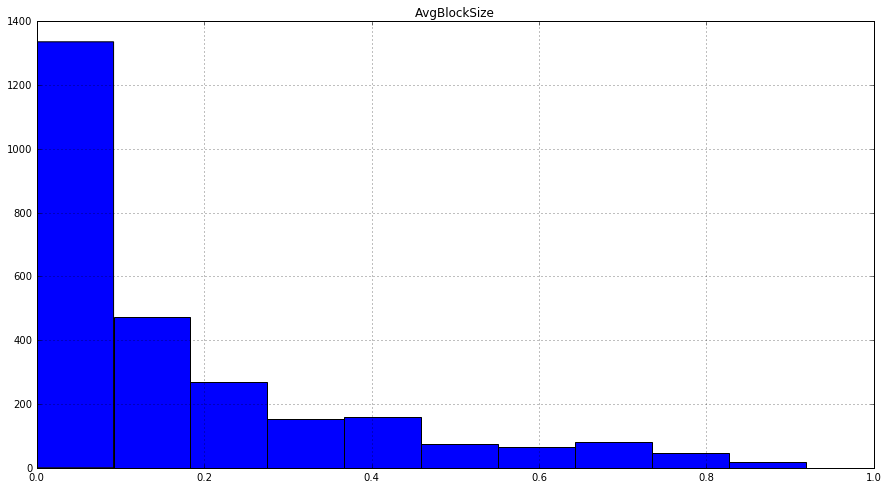
\includegraphics[width=1\linewidth]
    {gfx/avg-block-size-histogram}} 
  \caption{Average Block Size Histogram}
  \label{fig:avg-block-size-histogram}
\end{figure}

\begin{table}
  \myfloatalign
  \small
  \begin{tabularx}{\textwidth}{XX} 
    \toprule
    \tableheadline{Measure} & \tableheadline{Value} \\
    \midrule 
    count  & $2678$\\
    mean   & $0.165078$\\
    median & $0.092355$\\
    std    & $0.209430$\\
    min    & $0.000000$\\
    $25$\% & $0.000899$\\
    $50$\% & $0.092356$\\
    $75$\% & $0.242478$\\
    max    & $0.918519$\\
    \bottomrule
  \end{tabularx}
  \caption{Statistical values for 
    \textit{Average Block Size}}
  \label{tab:stats-avg-block-size}
\end{table}

\begin{figure}[bth]
  \myfloatalign
    {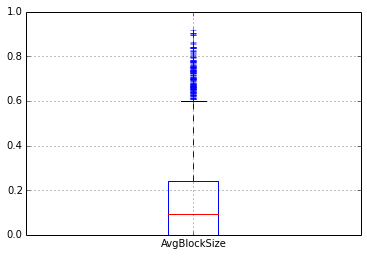
\includegraphics[width=1\linewidth]
      {gfx/avg-block-size-boxplot}}               
    \caption{Average Block Size Boxplot}
    \label{fig:avg-block-size-boxplot}
\end{figure}

\clearpage

%----------------------------------------------------------------------

\subsection{Bitcoin Days Destroyed}
\label{sec:bitcoin-days-destroyed}

\begin{figure}[bth]
  \myfloatalign
  {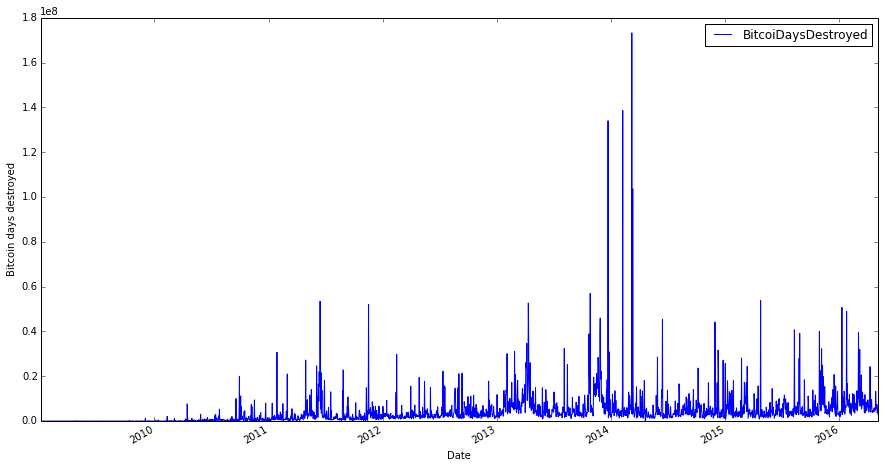
\includegraphics[width=1\linewidth]
    {gfx/bitcoin-days-destroyed-over-time}}
  \caption{Bitcoin Days Destroyed Over Time}
  \label{fig:bitcoin-days-destroyed-over-time}
\end{figure}

Bitcoin Days Destroyed is a weighted measure of aggregate economic
activity, placing value on transacted coins in proportion to the time
they have spent idle on the Bitcoin blockchain. For any given
transaction, Days Destroyed is calculated by multiplying its estimated
transaction value by the number of days since the coins within the
transaction were last spent. Bitcoin Days Destroyed is a useful proxy
for measuring growth in real value transacted on the Bitcoin
blockchain over time, since it controls for rapid movement of coins
between wallets (potentially owned by just one entity). One integer
data point each day, at 18:15:05, spanning from 03/01/2009 to
03/05/2016.

To better understand this variable we include a quote extracted from
\href{http://bitcoin.stackexchange.com/questions/845/what-are-bitcoin-days-destroyed}{Bitcoin
  Beta | Stack Exchange}:

``\textit{The idea of "bitcoin days destroyed" came about because it
  was realized that total transaction volume per day might be an
  inappropriate measure of the level of economic activity in Bitcoin.
  After all, someone could be sending the same money back and forth
  between their own addresses repeatedly. If you sent the same 50 btc
  back and forth 20 times, it would look like 1000 btc worth of
  activity, while in fact it represents almost nothing in terms of
  real transaction volume.}

\textit{With "bitcoin days destroyed", the idea is instead to give
  more weight to coins which haven't been spent in a while. To do
  this, you multiply the amount of each transaction by the number of
  days since those coins were last spent. So, 1 bitcoin that hasn't
  been spent in 100 days (1 bitcoin * 100 days) counts as much as 100
  bitcoins that were just spent yesterday (100 bitcoins * 1 day).
  Because you can think of these "bitcoin days" as building up over
  time until a transaction actually occurs, the actual measure is
  called "bitcoin days destroyed". This is believed to give a better
  indication of how much real economic activity is occurring on the
  bitcoin network.}

\textit{ So how well does it work? Well, it's still not perfect,
  because the other day I moved some coins out of a wallet they've
  been in for several months without spending them or giving them
  away. And some genuine businesses have very rapid turnover in
  bitcoins, so they're not being measured well by this method. But it
  does do a good job of filtering out the "noise" of bitcoins that are
  just "bouncing around" without really going anywhere. The graph of
  overall bitcoin days destroyed is believed to show that the genuine
  level of activity in the Bitcoin economy is continually
  increasing--it's not just one person experimenting by rapidly
  sending the same coins back and forth, flooding the network with
  meaningless chatter. Looks pretty good, hey?}''

\begin{table}
  \myfloatalign
  %\small
  \begin{tabularx}{\textwidth}{XX} 
    \toprule
    \tableheadline{Measure} & \tableheadline{Value} \\
    \midrule 
    count  & $2.679000e+03$ \\
    mean   & $4.146916e+06$ \\
    median & $2456794.0$ \\
    std    & $7.778546e+06$ \\
    min    & $0.000000e+00$ \\
    25\%   & $5.017520e+05$ \\
    50\%   & $2.456794e+06$ \\
    75\%   & $4.745530e+06$ \\
    max    & $1.732980e+08$ \\
    \bottomrule
  \end{tabularx}
  \caption{Statistical values for \textit{Bitcoin Days Destroyed}}
  \label{tab:bitcoin-days-destroyed}
\end{table}

\begin{figure}[bth]
  \myfloatalign
  {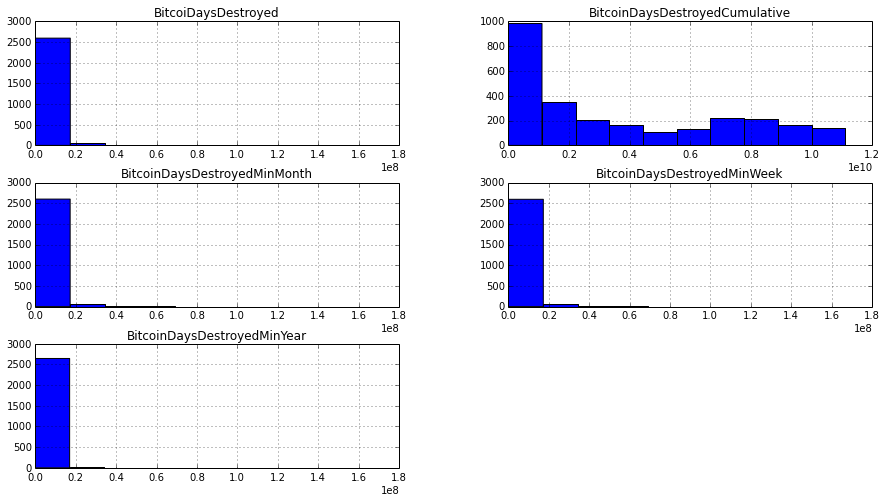
\includegraphics[width=1\linewidth]
    {gfx/bitcoin-days-destroyed-histogram}}
  \caption{Bitcoin Days Destroyed Histogram}
  \label{fig:bitcoin-days-destroyed-histogram}
\end{figure}

\begin{figure}[bth]
  \myfloatalign
  {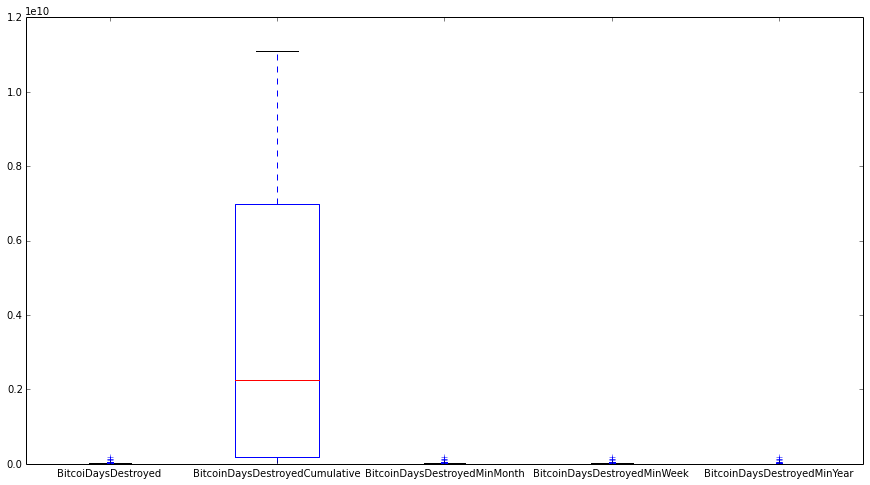
\includegraphics[width=1\linewidth]
    {gfx/bitcoin-days-destroyed-boxplot}}
  \caption{Bitcoin Days Destroyed Boxplot}
  \label{fig:bitcoin-days-destroyed-boxplot}
\end{figure}

\clearpage

%----------------------------------------------------------------------

\subsection{Bitcoin Days Destroyed Min Month}
\label{sec:bitcoin-days-destroyed-min-month}

\begin{figure}[bth]
  \myfloatalign
  {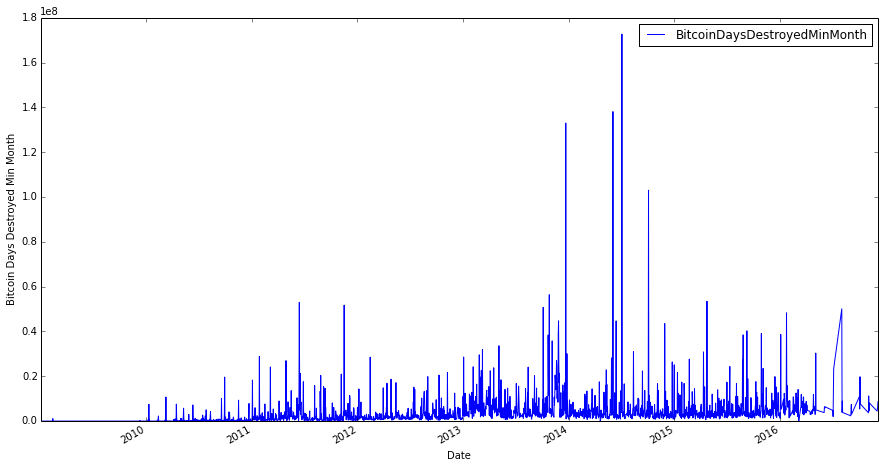
\includegraphics[width=1\linewidth]
    {gfx/bitcoin-days-destroyed-min-month-over-time}}
  \caption{Bitcoin Days Destroyed Min Month Over Time}
  \label{fig:bitcoin-days-destroyed-min-month-over-time}
\end{figure}

Bitcoin Days Destroyed filtered by minimum input age of 1 month. One
integer data point each day at 18:15:05, spanning from 03/01/2009 to
03/05/2016.  

\begin{table}
  \myfloatalign
  %\small
  \begin{tabularx}{\textwidth}{XX} 
    \toprule
    \tableheadline{Measure} & \tableheadline{Value} \\
    \midrule 
    count  & $2.679000e+03$ \\
    mean   & $3.649039e+06$ \\
    median & $1868139$      \\
    std    & $7.629002e+06$ \\
    min    & $0.000000e+00$ \\
    25\%   & $3.028175e+05$ \\
    50\%   & $1.868139e+06$ \\
    75\%   & $4.001042e+06$ \\
    max    & $1.727464e+08$ \\
    \bottomrule
  \end{tabularx}
  \caption{Statistical values for \textit{Bitcoin Days Destroyed Min Month}}
  \label{tab:bitcoin-days-destroyed-min-month}
\end{table}

\begin{figure}[bth]
  \myfloatalign
  {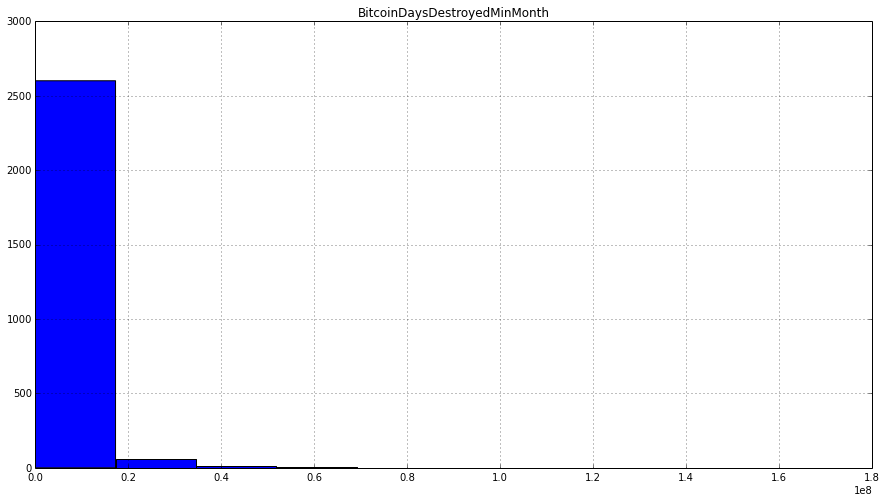
\includegraphics[width=1\linewidth]
    {gfx/bitcoin-days-destroyed-min-month-histogram}}
  \caption{Bitcoin Days Destroyed Min Month Histogram}
  \label{fig:bitcoin-days-destroyed-min-month-histogram}
\end{figure}

\begin{figure}[bth]
  \myfloatalign
  {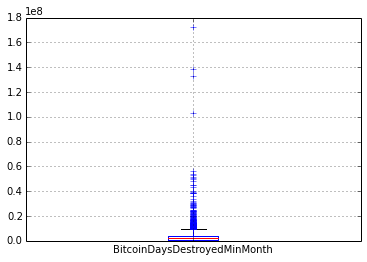
\includegraphics[width=1\linewidth]
    {gfx/bitcoin-days-destroyed-min-month-boxplot}}
  \caption{Bitcoin Days Destroyed Min Month Boxplot}
  \label{fig:bitcoin-days-destroyed-min-month-boxplot}
\end{figure}

\clearpage
%----------------------------------------------------------------------

\subsection{Bitcoin Days Destroyed Min Week}
\label{sec:bitcoin-days-destroyed-min-week}

\begin{figure}[bth]
  \myfloatalign
  {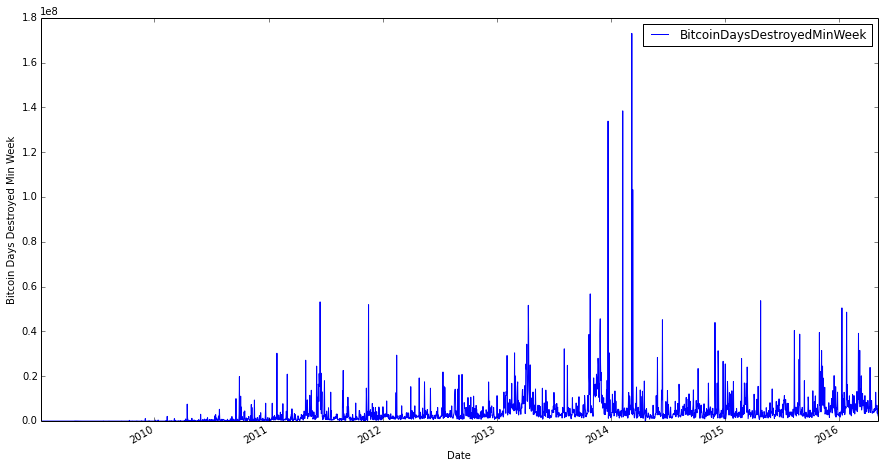
\includegraphics[width=1\linewidth]
    {gfx/bitcoin-days-destroyed-min-week-over-time}}
  \caption{Bitcoin Days Destroyed Min Week Over Time}
  \label{fig:bitcoin-days-destroyed-min-week-over-time}
\end{figure}

Bitcoin Days Destroyed filtered by minimum input age of 1 week. One
integer data point each day at 18:15:05, spanning from 03/01/2009 to
03/05/2016.

\begin{table}
  \myfloatalign
  %\small
  \begin{tabularx}{\textwidth}{XX} 
    \toprule
    \tableheadline{Measure} & \tableheadline{Value} \\
    \midrule 
    count  & $2.679000e+03$ \\
    mean   & $3.947443e+06$ \\
    median & $2210053$      \\
    std    & $7.721971e+06$ \\
    min    & $0.000000e+00$ \\
    25\%   & $4.384805e+05$ \\
    50\%   & $2.210053e+06$ \\
    75\%   & $4.454368e+06$ \\
    max    & $1.730718e+08$ \\
    \bottomrule
  \end{tabularx}
  \caption{Statistical values for \textit{Bitcoin Days Destroyed Min
      Week}} 
  \label{tab:bitcoin-days-destroyed-min-week}
\end{table}

\begin{figure}[bth]
  \myfloatalign
  {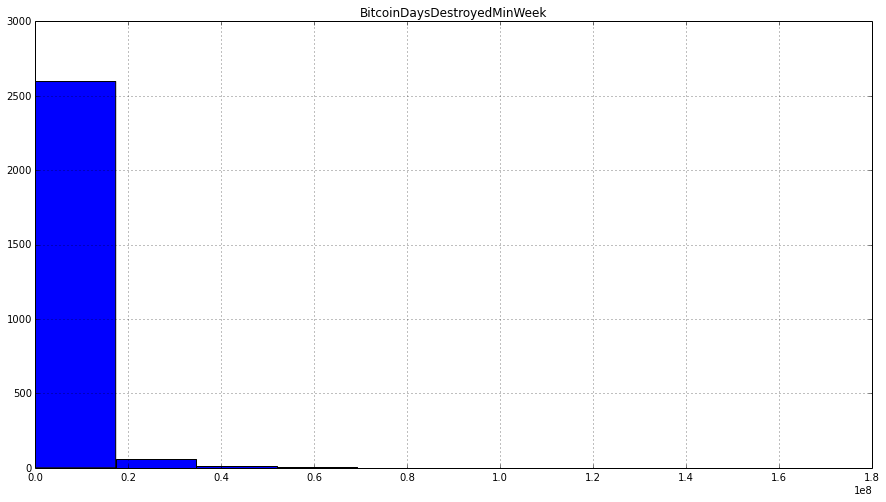
\includegraphics[width=1\linewidth]
    {gfx/bitcoin-days-destroyed-min-week-histogram}}
  \caption{Bitcoin Days Destroyed Min Week Histogram}
  \label{fig:bitcoin-days-destroyed-min-week-histogram}
\end{figure}

\begin{figure}[bth]
  \myfloatalign
  {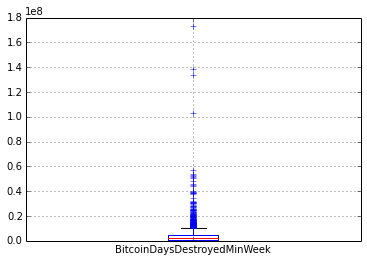
\includegraphics[width=1\linewidth]
    {gfx/bitcoin-days-destroyed-min-week-boxplot}}
  \caption{Bitcoin Days Destroyed Min Week Boxplot}
  \label{fig:bitcoin-days-destroyed-min-week-boxplot}
\end{figure}

\clearpage
%----------------------------------------------------------------------

\subsection{Bitcoin Days Destroyed Min Year}
\label{sec:bitcoin-days-destroyed-min-year}

\begin{figure}[bth]
  \myfloatalign
  {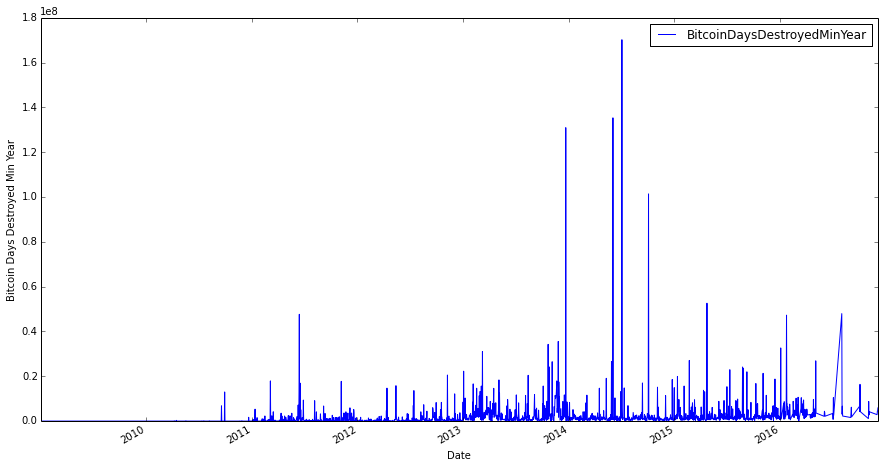
\includegraphics[width=1\linewidth]
    {gfx/bitcoin-days-destroyed-min-year-over-time}}
  \caption{Bitcoin Days Destroyed Min Year Over Time}
  \label{fig:bitcoin-days-destroyed-min-year-over-time}
\end{figure}

Bitcoin Days Destroyed filtered by minimum input age of 1 year. One
integer data point each day at 18:15:05, spanning from 03/01/2009 to
03/05/2016.

\begin{table}
  \myfloatalign
  %\small
  \begin{tabularx}{\textwidth}{XX} 
    \toprule
    \tableheadline{Measure} & \tableheadline{Value} \\
    \midrule 
    count  & $2.679000e+03$ \\
    mean   & $1.774081e+06$ \\
    median & $416483.0$     \\
    std    & $6.404385e+06$ \\
    min    & $0.000000e+00$ \\
    25\%   & $0.000000e+00$ \\
    50\%   & $4.164830e+05$ \\
    75\%   & $1.568172e+06$ \\
    max    & $1.702367e+08$ \\
    \bottomrule
  \end{tabularx}
  \caption{Statistical values for \textit{Bitcoin Days Destroyed Min
      Year}} 
  \label{tab:bitcoin-days-destroyed-min-year}
\end{table}

\begin{figure}[bth]
  \myfloatalign
  {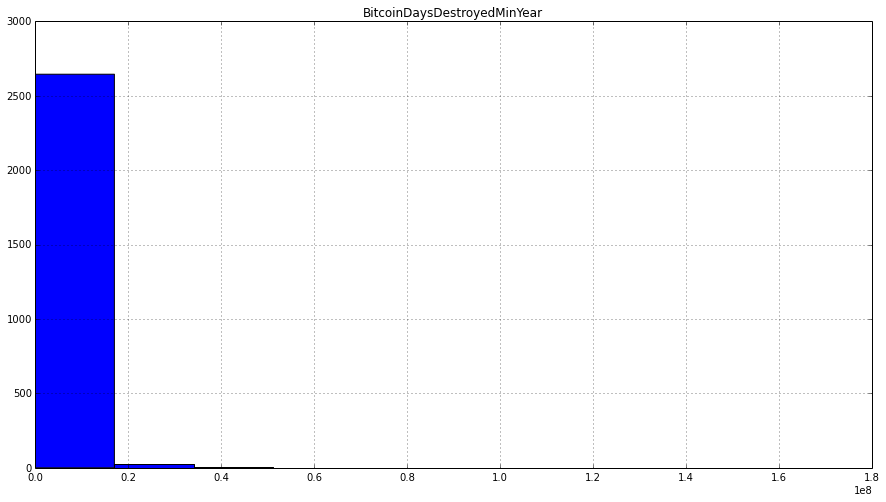
\includegraphics[width=1\linewidth]
    {gfx/bitcoin-days-destroyed-min-year-histogram}}
  \caption{Bitcoin Days Destroyed Min Year Histogram}
  \label{fig:bitcoin-days-destroyed-min-year-histogram}
\end{figure}

\begin{figure}[bth]
  \myfloatalign
  {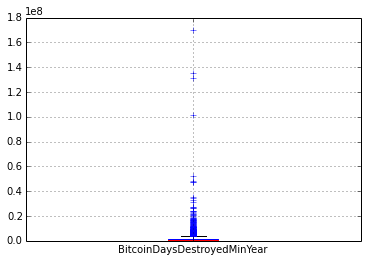
\includegraphics[width=1\linewidth]
    {gfx/bitcoin-days-destroyed-min-year-boxplot}}
  \caption{Bitcoin Days Destroyed Min Year Boxplot}
  \label{fig:bitcoin-days-destroyed-min-year-boxplot}
\end{figure}

\clearpage
%----------------------------------------------------------------------

\subsection{Bitcoin Days Destroyed Cumulative}
\label{sec:bitcoin-days-destroyed-cumulative}

\begin{figure}[bth]
  \myfloatalign
  {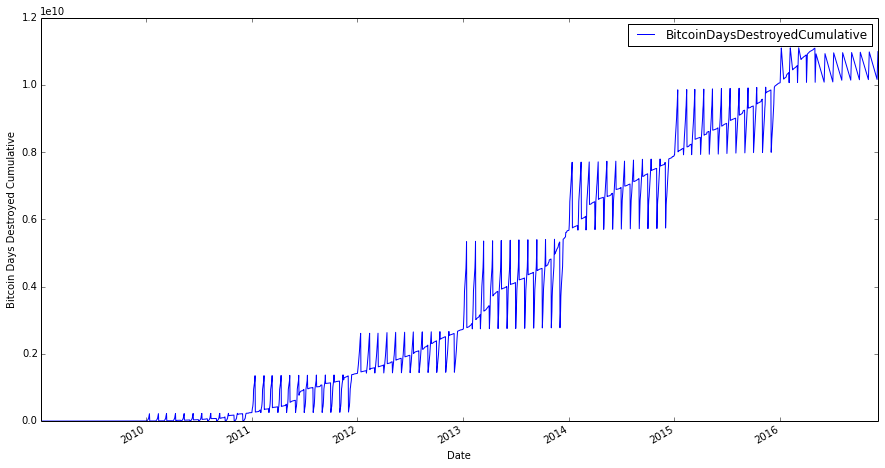
\includegraphics[width=1\linewidth]
    {gfx/bitcoin-days-destroyed-cumulative-over-time}}
  \caption{Bitcoin Days Destroyed Cumulative Over Time}
  \label{fig:bitcoin-days-destroyed-cumulative-over-time}
\end{figure}

Bitcoin Days Destroyed Cumulative acumulates all the bitcoins days
destroyed. That means that the increase of these variable shows the
increase in ``real'' transactions. In
\autoref{fig:bitcoin-days-destroyed-cumulative-over-time} we can see
that the value of this variable keeps growing, which leads us to think
that the ``real'' use of Bitcoin is also growin.

All the ``Bitcoin Days Destroyed'' variables are useful to disciminate
the ``real'' transaction between people and the rapid transaction
that can be done by traders for example.

The dataset comprises one integer data point each day, at
18:15:05, spanning from 03/01/2009 to 03/05/2016.

\begin{table}
  \myfloatalign
  %\small
  \begin{tabularx}{\textwidth}{XX} 
    \toprule
    \tableheadline{Measure} & \tableheadline{Value} \\
    \midrule 
    count  & $2.679000e+03$ \\
    mean   & $3.609471e+09$ \\
    median & $2265772771.0$ \\
    std    & $3.572547e+09$ \\
    min    & $0.000000e+00$ \\
    25\%   & $1.817693e+08$ \\
    50\%   & $2.265773e+09$ \\
    75\%   & $6.971917e+09$ \\
    max    & $1.110959e+10$ \\ 
    \bottomrule
  \end{tabularx}
  \caption{Statistical values for \textit{Bitcoin Days Destroyed Cumulative}}
  \label{tab:bitcoin-days-destroyed-cumulative}
\end{table}

\begin{figure}[bth]
  \myfloatalign
  {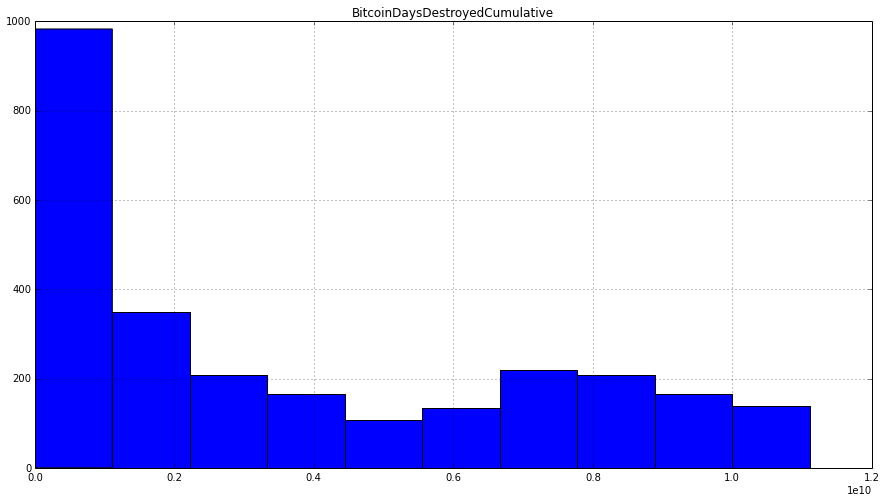
\includegraphics[width=1\linewidth]
    {gfx/bitcoin-days-destroyed-cumulative-histogram}}
  \caption{Bitcoin Days Destroyed Cumulative Histogram}
  \label{fig:bitcoin-days-destroyed-cumulative-histogram}
\end{figure}

\begin{figure}[bth]
  \myfloatalign
  {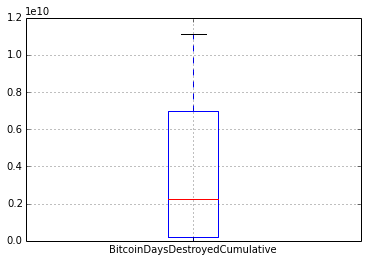
\includegraphics[width=1\linewidth]
    {gfx/bitcoin-days-destroyed-cumulative-boxplot}}
  \caption{Bitcoin Days Destroyed Cumulative Boxplot}
  \label{fig:bitcoin-days-destroyed-cumulative-boxplot}
\end{figure}

\clearpage
%----------------------------------------------------------------------

\subsection{Block Size}
\label{sec:block-size}

\begin{figure}[bth]
  \myfloatalign
  {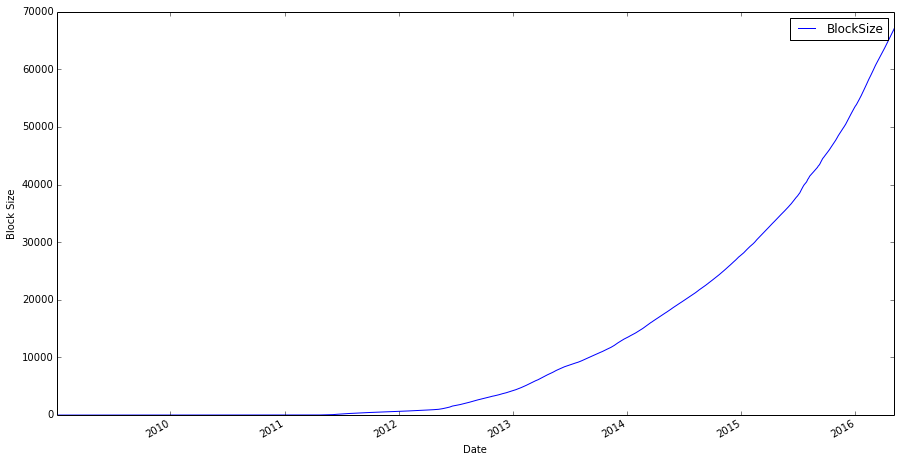
\includegraphics[width=1\linewidth]
    {gfx/block-size-over-time}}
  \caption{Block Size Over Time}
  \label{fig:block-size-over-time}
\end{figure}

The total size (in MB) of all block headers and transactions. Not
including database indexes. One real number data point each day, at
18:15:05, spanning from 03/01/2009 to 03/05/2016.

The total block size is increasing exponentialy as seen in
\autoref{fig:block-size-over-time}. This basically represents that the
total ammount of transactions are increasing at that rate.

\begin{table}
  \myfloatalign
  %\small
  \begin{tabularx}{\textwidth}{XX} 
    \toprule
    \tableheadline{Measure} & \tableheadline{Value} \\
    \midrule 
    count  & $2678.000000$       \\
    mean   & $9.727391$          \\
    median & $6.219650292785771$ \\
    std    & $13.268846$         \\
    min    & $0.000000$          \\
    25\%   & $1.301186$          \\
    50\%   & $6.219650$          \\
    75\%   & $10.401306$         \\
    max    & $90.202095$         \\
    \bottomrule
  \end{tabularx}
  \caption{Statistical values for \textit{Block Size}}
  \label{tab:block-size}
\end{table}

\begin{figure}[bth]
  \myfloatalign
  {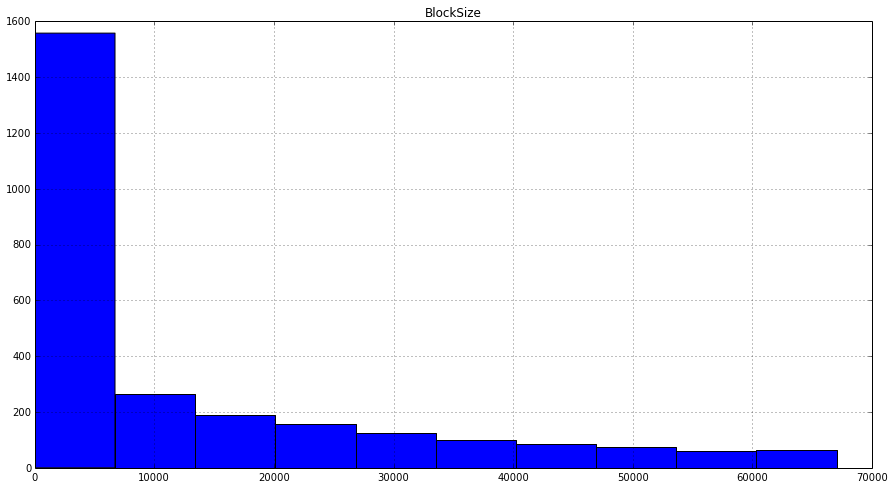
\includegraphics[width=1\linewidth]
    {gfx/block-size-histogram}}
  \caption{Block Size Histogram}
  \label{fig:block-size-histogram}
\end{figure}

\begin{figure}[bth]
  \myfloatalign
  {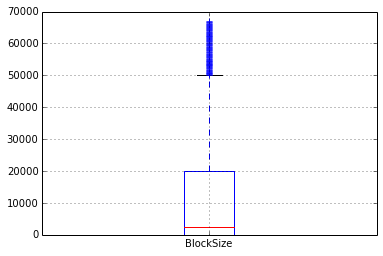
\includegraphics[width=1\linewidth]
    {gfx/block-size-boxplot}}
  \caption{Block Size Boxplot}
  \label{fig:block-size-boxplot}
\end{figure}

\clearpage
%----------------------------------------------------------------------

\subsection{Cost Per Transaction}
\label{sec:cost-per-transaction}

This variable shows miners revenue (in USD) divided by the number of
transactions. To better understand the fluctuations of \textit{Cost
  Per Transaction} show in
\autoref{fig:cost-per-transaction-over-time} we include the next
definition, found
\href{https://en.bitcoin.it/wiki/Transaction_fees}{here}:

\textit{``The transaction fee is processed by and received by the
  bitcoin miner. When a new bitcoin block is generated with a
  successful hash, the information for all of the transactions is
  included with the block and all transaction fees are collected by
  that user creating the block, who is free to assign those fees to
  himself.}

\textit{Transaction fees are voluntary on the part of the person
  making the bitcoin transaction, as the person attempting to make a
  transaction can include any fee or none at all in the transaction.
  On the other hand, nobody mining new bitcoins necessarily needs to
  accept the transactions and include them in the new block being
  created. The transaction fee is therefore an incentive on the part
  of the bitcoin user to make sure that a particular transaction will
  get included into the next block which is generated.''}

Knowing how the fees work in Bitcoin, we can see that the cost depends
on the will of the miner to accept or not the transaction. If we look
at \autoref{fig:n-transactions-over-time} we can see that there is
some correlation between the number of transactions been processed and
the cost of each transaction. The first peek in both figures coincide
around January/2011, after that, in mid 2011 there is a sustained
increase in the number of transactions, which in
\autoref{fig:cost-per-transaction-over-time} has a counterpart peek in
the cost of transactions, probably, because a lot of people wanted to
make transactions and the amount of miners were small. After that the
cost per transaction lowers and doesn't have a significant increase
till mid 2013. This increase is due to an increase in trade volume,
that can be seen clearly in \autoref{fig:trade-volume-over-time}. Next
to that, we see the biggest cost of cost per transaction so far, which
took place in the end of 2013 and start of 2014. This peek also occurs
simultaneously to a trade volume peek.

\begin{figure}[bth]
  \myfloatalign
  {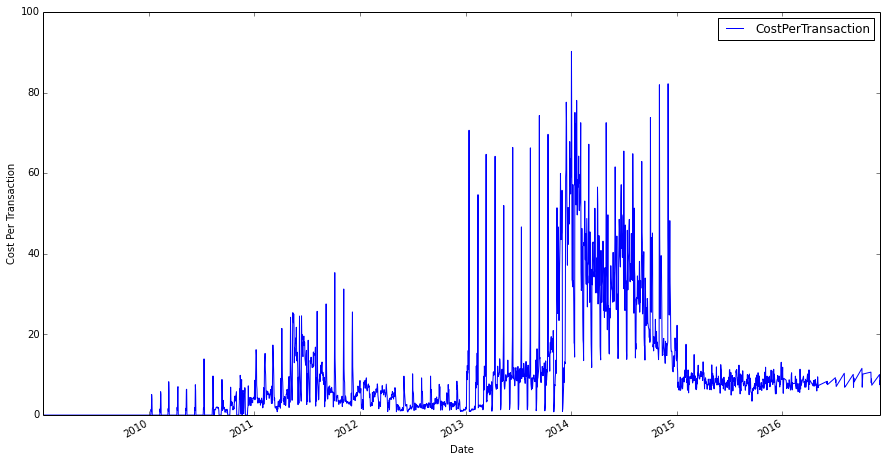
\includegraphics[width=1\linewidth]
    {gfx/cost-per-transaction-over-time}}
  \caption{Cost Per Transaction Over Time}
  \label{fig:cost-per-transaction-over-time}
\end{figure}

The dataset comprises one real number data point each day, at
18:15:05, spanning from 03/01/2009 to 03/05/2016.

\begin{table}
  \myfloatalign
  %\small
  \begin{tabularx}{\textwidth}{XX} 
    \toprule
    \tableheadline{Measure} & \tableheadline{Value} \\
    \midrule 
    count  & $2678$ \\
    mean   & $9.727391$    \\
    median & $6.21965$     \\
    std    & $13.268846$   \\
    min    & $0$    \\
    $25$\  & $1.301186$    \\
    $50$\  & $6.219650$    \\
    $75$\  & $10.401306$   \\
    max    & $90.202095$   \\
    \bottomrule
  \end{tabularx}
  \caption{Statistical values for \textit{Cost Per Transaction}}
  \label{tab:cost-per-transaction}
\end{table}

\begin{figure}[bth]
  \myfloatalign
  {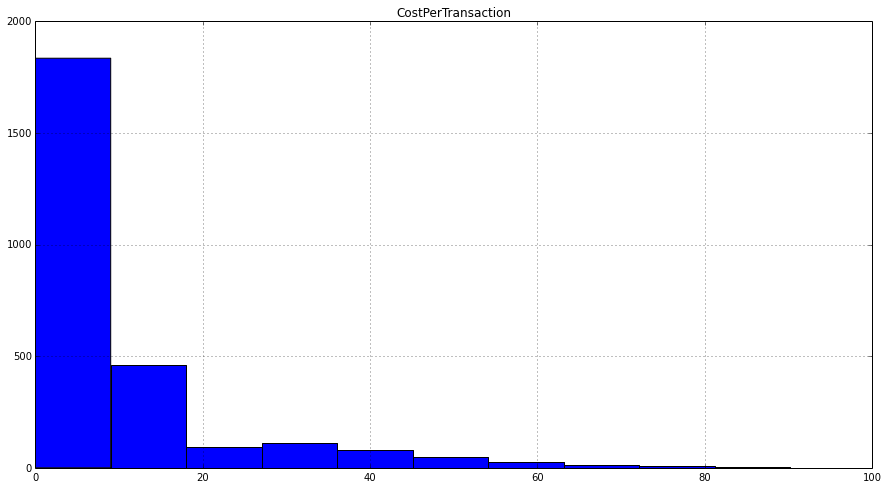
\includegraphics[width=1\linewidth]
    {gfx/cost-per-transaction-histogram}}
  \caption{Cost Per Transaction Histogram}
  \label{fig:cost-per-transaction-histogram}
\end{figure}

\begin{figure}[bth]
  \myfloatalign
  {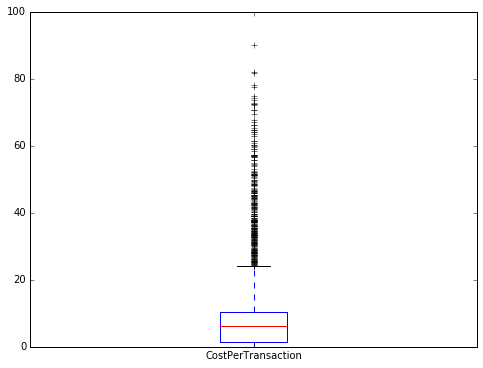
\includegraphics[width=1\linewidth]
    {gfx/cost-per-transaction-boxplot}}
  \caption{Cost Per Transaction Boxplot}
  \label{fig:cost-per-transaction-boxplot}
\end{figure}

\clearpage
%----------------------------------------------------------------------

\subsection{Cost Per Transaction Percent}
\label{sec:cost-per-transaction-percent}

\begin{figure}[bth]
  \myfloatalign
  {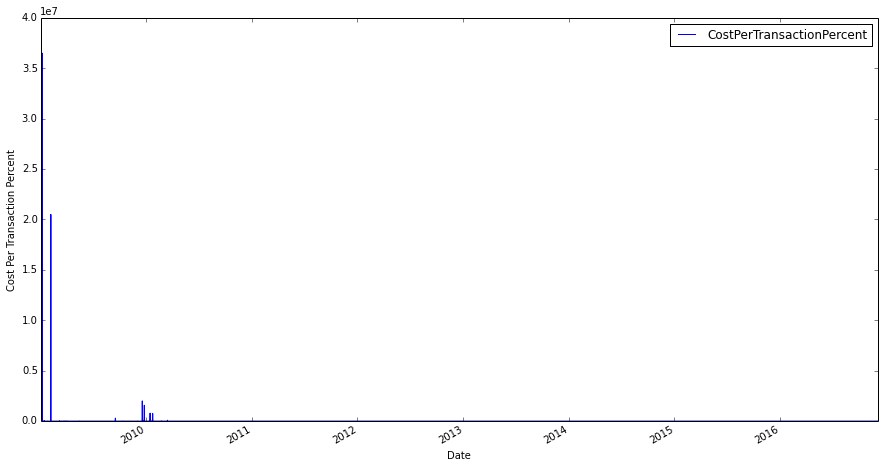
\includegraphics[width=1\linewidth]
    {gfx/cost-per-transaction-percent-over-time}}
  \caption{Cost Per Transaction Percent Over Time}
  \label{fig:cost-per-transaction-percent-over-time}
\end{figure}

This variable shows miners revenue as percentage of the transaction
volume. Basically what
\autoref{fig:cost-per-transaction-percent-over-time} shows is that
over time, the transactions fees are decreasing with respect to the
transaction amount itself. The median, shown in
\autoref{tab:cost-per-transaction-percent}, is $3.283375136886966\%$,
which reflects the percent of transaction that is used mostly in all
Bitcoin transactions.

The dataset comprises one real number data point each day, at
18:15:05, spanning from 03/01/2009 to 03/05/2016.

\begin{table}
  \myfloatalign
  %\small
  \begin{tabularx}{\textwidth}{XX} 
    \toprule
    \tableheadline{Measure} & \tableheadline{Value} \\
    \midrule 
    count  & $2678.000000$       \\
    mean   & $23603.541449$      \\
    median & $3.283375136886966$ \\
    std    & $810554.930805$     \\
    min    & $0.000000$          \\
    25\%   & $1.580112$          \\
    50\%   & $3.283375$          \\
    75\%   & $9.606991$          \\
    max    & $36500000.000000$   \\
    \bottomrule
  \end{tabularx}
  \caption{Statistical values for \textit{Cost Per Transaction Percent}}
  \label{tab:cost-per-transaction-percent}
\end{table}

\begin{figure}[bth]
  \myfloatalign
  {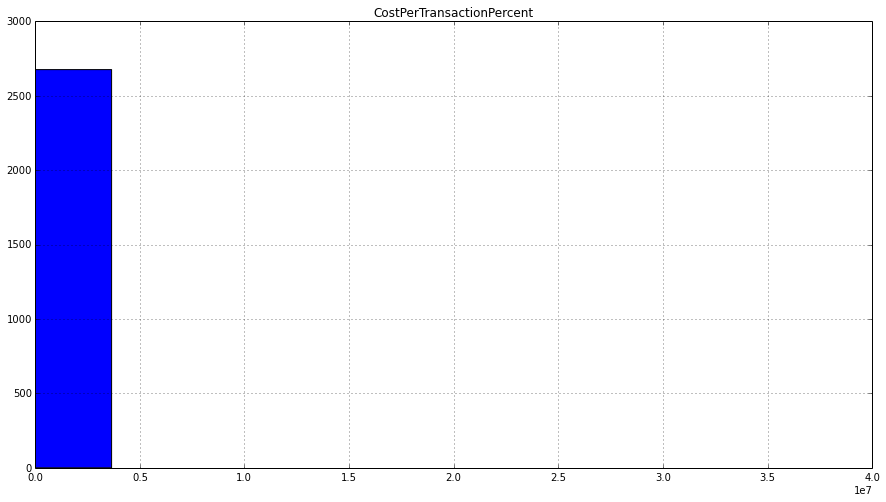
\includegraphics[width=1\linewidth]
    {gfx/cost-per-transaction-percent-histogram}}
  \caption{Cost Per Transaction Percent Histogram}
  \label{fig:cost-per-transaction-percent-histogram}
\end{figure}

\begin{figure}[bth]
  \myfloatalign
  {\includegraphics[width=1\linewidth]
    {gfx/cost-per-transaction-percent-boxplot}}
  \caption{Cost Per Transaction Percent Boxplot}
  \label{fig:cost-per-transaction-percent-boxplot}
\end{figure}

\clearpage
%----------------------------------------------------------------------

\subsection{Difficulty}
\label{sec:difficulty}

\begin{figure}[bth]
  \myfloatalign
  {\includegraphics[width=1\linewidth]
    {gfx/difficulty-over-time}}
  \caption{Difficulty Over Time}
  \label{fig:difficulty-over-time}
\end{figure}

A relative measure of how difficult it is to find a new block. The
difficulty is adjusted periodically as a function of how much hashing
power has been deployed by the network of miners. That can be seen
looking at how similar are \autoref{fig:difficulty-over-time} and
\autoref{fig:hash-rate-over-time}. The graphic representing the
difficulty has a discrete shape, that is because the difficulty is
adjusted automatically every 2016 blocks, and changes equally for the
entire Bitcoin network. Until 2014, the difficulty of mining was
very low, it started to raise probably because the trade volume in the
end of 2013 and start of 2014 was approximately 70.000.000\$, which
attracted professional miners with a greater processing power, those
creating more and more blocks and augmenting the difficulty of mining.

The dataset comprises one real number data point each day, at
18:15:05, spanning from 03/01/2009 to 03/05/2016.

\begin{table}
  \myfloatalign
  %\small
  \begin{tabularx}{\textwidth}{XX} 
    \toprule
    \tableheadline{Measure} & \tableheadline{Value} \\
    \midrule 
    count  & $2.678000e+03$      \\
    mean   & $1.683580e+10$      \\
    median & $2440642.606915964$ \\
    std    & $3.561708e+10$      \\
    min    & $0.000000e+00$      \\
    25\%   & $3.091737e+03$      \\
    50\%   & $2.440643e+06$      \\
    75\%   & $1.681846e+10$      \\
    max    & $1.786783e+11$      \\
    \bottomrule
  \end{tabularx}
  \caption{Statistical values for \textit{Difficulty}}
  \label{tab:difficulty}
\end{table}

\begin{figure}[bth]
  \myfloatalign
  {\includegraphics[width=1\linewidth]
    {gfx/difficulty-histogram}}
  \caption{Difficulty Histogram}
  \label{fig:difficulty-histogram}
\end{figure}

\begin{figure}[bth]
  \myfloatalign
  {\includegraphics[width=1\linewidth]
    {gfx/difficulty-boxplot}}
  \caption{Difficulty Boxplot}
  \label{fig:difficulty-boxplot}
\end{figure}

\clearpage
%----------------------------------------------------------------------

\subsection{Estimated Transaction Volume}
\label{sec:estimated-transaction-volume}

\begin{figure}[bth]
  \myfloatalign
  {\includegraphics[width=1\linewidth]
    {gfx/estimated-transaction-volume-over-time}}
  \caption{Estimated Transaction Volume Over Time}
  \label{fig:estimated-transaction-volume-over-time}
\end{figure}

The total estimated value of transactions on the Bitcoin blockchain
(does not include coins returned to sender as change). The transaction
volume represented in
\autoref{fig:estimated-transaction-volume-over-time} is very slowly
increasing, meaning that more transactions in Bitcoin are processed.
However, it doesn't represent the actual value of transactions,
because people think in their local currency when trading or shopping,
and Bitcoin's value is volatile. Is more useful the next variable,
\textit{Estimated Transaction Volume USD} that gives as tells the
actual value of transactions. The peak that happened in 2012 wouldn't
occur easily today due to the current value of Bitcoin.

The data-set comprises one integer data point each day, at
18:15:05, spanning from 03/01/2009 to 03/05/2016.

\begin{table}
  \myfloatalign
  %\small
  \begin{tabularx}{\textwidth}{XX} 
    \toprule
    \tableheadline{Measure} & \tableheadline{Value} \\
    \midrule 
    count  & $2679.000000$    \\
    mean   & $157340.920119$  \\
    median & $118843.0$       \\
    std    & $282285.024788$  \\
    min    & $0.000000$       \\
    $25$\% & $30553.000000$   \\
    $50$\% & $118843.000000$  \\
    $75$\% & $210442.000000$  \\
    max    & $5825066.000000$ \\
    \bottomrule
  \end{tabularx}
  \caption{Statistical values for \textit{Estimated Transaction Volume}}
  \label{tab:estimated-transaction-volume}
\end{table}

\begin{figure}[bth]
  \myfloatalign
  {\includegraphics[width=1\linewidth]
    {gfx/estimated-transaction-volume-histogram}}
  \caption{Estimated Transaction Volume Histogram}
  \label{fig:estimated-transaction-volume-histogram}
\end{figure}

\begin{figure}[bth]
  \myfloatalign
  {\includegraphics[width=1\linewidth]
    {gfx/estimated-transaction-volume-boxplot}}
  \caption{Estimated Transaction Volume Boxplot}
  \label{fig:estimated-transaction-volume-boxplot}
\end{figure}

\clearpage
%----------------------------------------------------------------------

\subsection{Estimated Transaction Volume USD}
\label{sec:estimated-transaction-volume-usd}

\begin{figure}[bth]
  \myfloatalign
  {\includegraphics[width=1\linewidth]
    {gfx/estimated-transaction-volume-usd-over-time}}
  \caption{Estimated Transaction Volume USD Over Time}
  \label{fig:estimated-transaction-volume-usd-over-time}
\end{figure}

The Estimated Transaction Volume in USD value, shown in
\autoref{fig:estimated-transaction-volume-usd-over-time}, can be
explained by the average value of Bitcoin, shown in
\autoref{fig:market-price-over-time}, because nearly all the events
are paired in the two figures. There is a small increase in estimated
transaction volume in USD in mid 2011 at the same time than the
average price of Bitcoin increases. Later on, in 2013 there is a
bigger increase in estimated volume that is also reflected in the
average price. Then we have the two biggest peaks around January of
2014 coinciding with the higher average value of Bitcoin (also
represented in two peaks). After that there is decrease in average
price and estimated volume till 2016 where Bitcoin average price
starts to increase at the same time that the estimate transaction
volume increases.

This data-set comprises one integer data point each day, at 18:15:05,
spanning from 03/01/2009 to 03/05/2016.

\begin{table}
  \myfloatalign
  %\small
  \begin{tabularx}{\textwidth}{XX} 
    \toprule
    \tableheadline{Measure} & \tableheadline{Value} \\
    \midrule 
    count  & $2.679000e+03$ \\
    median & $2481424.0$    \\
    mean   & $3.018470e+07$ \\
    std    & $4.923048e+07$ \\
    min    & $0.000000e+00$ \\
    $25$\% & $5.086000e+03$ \\
    $50$\% & $2.481424e+06$ \\
    $75$\% & $4.761785e+07$ \\
    max    & $5.787707e+08$ \\
    \bottomrule
  \end{tabularx}
  \caption{Statistical values for \textit{Estimated Transaction Volume USD}}
  \label{tab:estimated-transaction-volume-usd}
\end{table}

\begin{figure}[bth]
  \myfloatalign
  {\includegraphics[width=1\linewidth]
    {gfx/estimated-transaction-volume-usd-histogram}}
  \caption{Estimated Transaction Volume USD Histogram}
  \label{fig:estimated-transaction-volume-usd-histogram}
\end{figure}

\begin{figure}[bth]
  \myfloatalign
  {\includegraphics[width=1\linewidth]
    {gfx/estimated-transaction-volume-usd-boxplot}}
  \caption{Estimated Transaction Volume USD Boxplot}
  \label{fig:estimated-transaction-volume-usd-boxplot}
\end{figure}

\clearpage

%----------------------------------------------------------------------

\subsection{Euro price in USD}
\label{sec:euro-price-in-usd}

\begin{figure}[bth]
  \myfloatalign
  {\includegraphics[width=1\linewidth]
    {gfx/euro-price-in-usd-over-time}} 
  \caption{Euro price in USD Over Time}
  \label{fig:euro-price-in-usd-over-time}
\end{figure}

Euro price in USD provided by the European Central Bank from the
creation of the Euro. One real data entry per day, spanning from
04/01/1999 to 10/05/2016.

This dataset has latent values. We have used interpolation in order to
fill the missing values.

As shown in \autoref{fig:euro-price-in-usd-over-time} the value of Euro
has been above that of the USD from its creation, been the period of
2000 through 2003 its closer price to each other. From 2003 to 2007
the price of the Euro increased, coinciding with an increase on the
interest imposed by the BCE. This increase in the interest of the
credits is followed by the collapse of the housing bubble in 2007,
where the price of the Euro kept increasing, altough the interest was
maintained by the BCE until 2009 where the BCE started to lower it.
The increase in the Euro price is probably due to strategies of the
Federal Reserve to lower the price of the USD. Finally in 2015, the
BCE lowered the interests of credits approaching the $0.0\%$, and
that's reflected with a decrease in the price of the Euro with respect
to USD.

\begin{table}
  \myfloatalign
  %\small
  \begin{tabularx}{\textwidth}{XX} 
    \toprule
    \tableheadline{Measure} & \tableheadline{Value} \\
    \midrule 
    count & 4443\\
    mean  & 1.216306\\
    median & 1.2579\\
    std   & 0.177679\\
    min   & 0.825200\\
    25\%  & 1.088300\\
    50\%  & 1.257900\\
    75\%  & 1.345050\\
    max   & 1.599000\\
    \bottomrule
  \end{tabularx}
  \caption{Statistical values for \textit{Euro price in USD}}
  \label{tab:euro-price-in-usd}
\end{table}

There are 62 missing values in the data which has been interpolated
after obtaining the descriptive variables of
\autoref{tab:euro-price-in-usd}

\begin{figure}[bth]
  \myfloatalign
  {\includegraphics[width=1\linewidth]
    {gfx/euro-price-in-usd-histogram}} 
  \caption{Euro price in USD Histogram}
  \label{fig:euro-price-in-usd-histogram}
\end{figure}

\begin{figure}[bth]
  \myfloatalign
  {\includegraphics[width=1\linewidth]
    {gfx/euro-price-in-usd-boxplot}}
  \caption{Euro price in USD Boxplot}
  \label{fig:euro-price-in-usd-boxplot}
\end{figure}

\clearpage

%----------------------------------------------------------------------

\subsection{Hash Rate}
\label{sec:hash-rate}

\begin{figure}[bth]
  \myfloatalign
  {\includegraphics[width=1\linewidth]
    {gfx/hash-rate-over-time}}
  \caption{Hash Rate Over Time}
  \label{fig:hash-rate-over-time}
\end{figure}

The estimated number of giga hashes per second (billions of hashes per
second) the Bitcoin network is performing. The chart in
\autoref{fig:hash-rate-over-time} shows us how mining really started
when Bitcoin raised to its highest value around 2014, reaching more
than 1000\$ per BTC. From that point on, the processing to mining has
increased at approximately $0.2 \times 10^9$ hashes per second, and in
2016, at the same time that the Bitcoin price is starting to increase,
the hash rate started to grow at $1 \times 10^9$ hashes per second in
just a few months. 

This data-set comprises one real number data point each day, at
18:15:05, spanning from 03/01/2009 to 03/05/2016.

\begin{table}
  \myfloatalign
  %\small
  \begin{tabularx}{\textwidth}{XX}
    \toprule
    \tableheadline{Measure} & \tableheadline{Value} \\
    \midrule
    count  & $2.678000e+03$      \\
    mean   & $1.265485e+08$      \\
    median & $19063.08687085293$ \\
    std    & $2.683517e+08$      \\
    min    & $0.000000e+00$      \\
    $25$\% & $2.973922e+01$      \\
    $50$\% & $1.906309e+04$      \\
    $75$\% & $1.250993e+08$      \\
    max    & $1.465554e+09$      \\
    \bottomrule
  \end{tabularx}
  \caption{Statistical values for \textit{Hash Rate}}
  \label{tab:hash-rate}
\end{table}

\begin{figure}[bth]
  \myfloatalign
  {\includegraphics[width=1\linewidth]
    {gfx/hash-rate-histogram}}
  \caption{Hash Rate Histogram}
  \label{fig:hash-rate-histogram}
\end{figure}

\begin{figure}[bth]
  \myfloatalign
  {\includegraphics[width=1\linewidth]
    {gfx/hash-rate-boxplot}}
  \caption{Hash Rate Boxplot}
  \label{fig:hash-rate-boxplot}
\end{figure}

\clearpage
%----------------------------------------------------------------------

\subsection{Market Capitalization}
\label{sec:market-cap}

\begin{figure}[bth]
  \myfloatalign
  {\includegraphics[width=1\linewidth]
    {gfx/market-cap-over-time}}
  \caption{Market Capitalization Over Time}
  \label{fig:market-cap-over-time}
\end{figure}

The total USD value of bitcoin supply in circulation, as calculated by
the daily average market price across major exchanges. This variable
is related to many others, starting with the Bitcoin market price,
with is virtually the same as this one, the number of transactions,
that can explain the fluctuations in the Bitcoin price and different
events. In March 9, 2011, the Bitcoin reaches parity with USD which is
shown in a timid growth in market capitalization followed by a
decrease. After that there isn't a big growth until 2013, where
several things happen, Mega, the cloud storage service, starts
accepting Bitcoins, Internet Archive starts accepting Bitcoins, a new
food service \href{PizzaForCoins.com}{PizzaForCoins.com} accepts
Bitcoins as a payment for food, CoinDesk is launched by Spotify
investor and Coinbase receives 5 million USD in funding. This, and
several other events increase the market capitalization for Bitcoin.

After that there is a decrease in market capitalization of Bitcoin,
maybe because MtGox, the largest exchange operator at the time, was
seized by The United States Department of Homeland Security.

In the second half of 2013, various events happen that can be the
cause of the raise of Bitcoin market capitalization, first, in August
6th, Bitcoin is ruled currency by a Texas judge, then in August 20th,
Bitcoin is ruled as private money in Germany, then in August 28th,
RoboCoin, a Bitcoin ATM manufacturer, starts accepting orders. This
can be the cause of the huge peek at the end of 2013 and start of
2014. There are no clear events in the Bitcoin history that explain
the period after 2014, which leads us to think that the price has been
fluctuating due to trading strategies.

This data-set comprises one real number data point each day, at
18:15:05, spanning from 03/01/2009 to 03/05/2016.

\begin{table}
  \myfloatalign
  %\small
  \begin{tabularx}{\textwidth}{XX} 
    \toprule
    \tableheadline{Measure} & \tableheadline{Value} \\
    \midrule 
    count  & $2.678000e+03$  \\
    mean   & $2.072915e+09$  \\
    median & $115624066.175$ \\
    std    & $2.879009e+09$  \\
    min    & $0.000000e+00$  \\
    $25$\% & $1.005470e+06$  \\
    $50$\% & $1.156241e+08$  \\
    $75$\% & $3.850512e+09$  \\
    max    & $1.390005e+10$  \\
    \bottomrule
  \end{tabularx}
  \caption{Statistical values for \textit{Market Capitalization}}
  \label{tab:market-cap}
\end{table}

\begin{figure}[bth]
  \myfloatalign
  {\includegraphics[width=1\linewidth]
    {gfx/market-cap-histogram}}
  \caption{Market Capitalization Histogram}
  \label{fig:market-cap-histogram}
\end{figure}

\begin{figure}[bth]
  \myfloatalign
  {\includegraphics[width=1\linewidth]
    {gfx/market-cap-boxplot}}
  \caption{Market Capitalization Boxplot}
  \label{fig:market-cap-boxplot}
\end{figure}

\clearpage
%----------------------------------------------------------------------

\subsection{Market Price}
\label{sec:market-price}

\begin{figure}[bth]
  \myfloatalign
  {\includegraphics[width=1\linewidth]
    {gfx/market-price-over-time}}
  \caption{Market Price Over Time}
  \label{fig:market-price-over-time}
\end{figure}

Average USD market price across major Bitcoin exchanges.
\autoref{fig:market-price-over-time} is identical to the one in
\autoref{fig:market-cap-over-time} except for the scale. The same
events that produced the market capitalization fluctuation apply to
the market price. Added to that, the average market price across mayor
Bitcoin exchange operators is a variable very closely related to the
market capitalization of Bitcoin.

Is important to note how volatile is the Bitcoin average price,
ranging from nearly $0$ USD to $1100$ USD in just a year, and now, in
2016 fluctuating in a range bigger than $10$ USD on average. This
fluctuations, if predicted, can be very profitable for the trader. 

The data-set comprises one real number data point each day, at
18:15:05, spanning from 03/01/2009 to 03/05/2016.

\begin{table}
  \myfloatalign
  %\small
  \begin{tabularx}{\textwidth}{XX} 
    \toprule
    \tableheadline{Measure} & \tableheadline{Value} \\
    \midrule 
    count  & $2678.000000$ \\
    mean   & $155.924369$  \\
    median & $12.37856$    \\
    std    & $218.563332$  \\
    min    & $0.000000$    \\
    $25$\% & $0.209250$    \\
    $50$\% & $12.378560$   \\
    $75$\% & $271.335000$  \\
    max    & $1151.000000$ \\
    \bottomrule
  \end{tabularx}
  \caption{Statistical values for \textit{Market Price}}
  \label{tab:market-price}
\end{table}

\begin{figure}[bth]
  \myfloatalign
  {\includegraphics[width=1\linewidth]
    {gfx/market-price-histogram}}
  \caption{Market Price Histogram}
  \label{fig:market-price-histogram}
\end{figure}

\begin{figure}[bth]
  \myfloatalign
  {\includegraphics[width=1\linewidth]
    {gfx/market-price-boxplot}}
  \caption{Market Price Boxplot}
  \label{fig:market-price-boxplot}
\end{figure}

\clearpage
%----------------------------------------------------------------------

\subsection{Median Confirmation Time}
\label{sec:median-confirmation-time}

\begin{figure}[bth]
  \myfloatalign
  {\includegraphics[width=1\linewidth]
    {gfx/median-confirmation-time-over-time}}
  \caption{Median Confirmation Time Over Time}
  \label{fig:median-confirmation-time-over-time}
\end{figure}

The median time for a transaction to be accepted into a mined block
and added to the public ledger (note: only includes transactions with
miner fees). Until the end of 2011, the confirmation time is
negligible. There is an important event that can be related to the
growth of the median confirmation time, and that is the largest
Bitcoin fee in a single transaction, in December 12, 171 Bitcoins was
paids as fee in block 157235.

If we look at \autoref{fig:median-confirmation-time-over-time} there
is a peak in mid 2012, that can coincide with the increase in number
of transactions seen in \autoref{fig:n-transactions-over-time}. After
that even though the number of transactions is growing, there is also
in increment in the hash rate, so the number of transactions can be
included in blocks thanks to the amount of miners and their processing
power.

 One real number data point each day, at 18:15:05,
spanning from 03/01/2009 to 03/05/2016.

\begin{table}
  \myfloatalign
  %\small
  \begin{tabularx}{\textwidth}{XX} 
    \toprule
    \tableheadline{Measure} & \tableheadline{Value} \\
    \midrule 
    count  & $2678.000000$ \\
    mean   & $5.385540$    \\
    median & $6.975$       \\
    std    & $4.859709$    \\
    min    & $0.000000$    \\
    $25$\% & $0.000000$    \\
    $50$\% & $6.975000$    \\
    $75$\% & $8.500000$    \\
    max    & $47.733333$   \\
    \bottomrule
  \end{tabularx}
  \caption{Statistical values for 
    \textit{Median Confirmation Time}}
  \label{tab:median-confirmation-time}
\end{table}

\begin{figure}[bth]
  \myfloatalign
  {\includegraphics[width=1\linewidth]
    {gfx/median-confirmation-time-histogram}}
  \caption{Median Confirmation Time Histogram}
  \label{fig:median-confirmation-time-histogram}
\end{figure}

\begin{figure}[bth]
  \myfloatalign
  {\includegraphics[width=1\linewidth]
    {gfx/median-confirmation-time-boxplot}}
  \caption{Median Confirmation Time Boxplot}
  \label{fig:median-confirmation-time-boxplot}
\end{figure}

\clearpage
%----------------------------------------------------------------------

\subsection{Miners Revenue}
\label{sec:miners-revenue}

\begin{figure}[bth]
  \myfloatalign
  {\includegraphics[width=1\linewidth]
    {gfx/miners-revenue-over-time}}
  \caption{Miners Revenue Over Time}
  \label{fig:miners-revenue-over-time}
\end{figure}

Total value of coinbase block rewards and transaction fees paid to
miners, expressed in USD. To understand the rewards and fees, we
include this quote, extracted the 1st of June of 2016 from
\href{https://en.bitcoin.it/wiki/Mining}{https://en.bitcoin.it/wiki/Mining}:

\textit{``When a block is discovered, the discoverer may award
  themselves a certain number of bitcoins, which is agreed-upon by
  everyone in the network. Currently this bounty is 25 bitcoins; this
  value will halve every 210,000 blocks. [...]. } 

\textit{Additionally, the miner is awarded the fees paid by users
  sending transactions. The fee is an incentive for the miner to
  include the transaction in their block. In the future, as the number
  of new bitcoins miners are allowed to create in each block dwindles,
  the fees will make up a much more important percentage of mining
  income.''}

Taking the previous quote into consideration, we know that the miner
reward is fixed, so its fluctuation will depend upon the price of the
Bitcoin itself, therefore the resemblance between miners revenue
(\autoref{fig:miners-revenue-over-time}) and Bitcoin price
(\autoref{fig:market-price-over-time}).

In 2016, the transaction fees represent a very small amount of the
BTCs of the miners revenue. We can see in
\autoref{tab:cost-per-transaction} that the average transaction has a
value of $9.727391$. On the other hand, the average number of
transactions per block $306.632248$. Thus the expected revenue due to
fees of a single miner is $9.727391 \times 306.632248 = $
$2982.7317695049683$ USD.

If we analyze the revenue thanks to the reward of discovering a block
we have that the average market price of the
Bitcoin(\autoref{tab:market-price}) is $155.924369$ USD and the reward
is $25$ BTC per block discovered, that makes an amount of $155.924369
\times 25 = 3898.109225$ USD per block discovered. Added to that, we
have to keep in mind that, as of June the $2^{nd}$, the current price
of Bitcoin is $536.99$ USD, which makes the rewards value increase to
$536.99 \times 25 = 13424.75$ USD per blocked discovered. We can
conclude that nowadays, the main source of revenues for miners is the
block discovery, but in the future, as it goes getting harder to
discover blocks, the fees will start to be an important source of
income for miners. 

This data-set comprises one real number data point each day, at
18:15:05, spanning from 03/01/2009 to 03/05/2016.

\begin{table}
  \myfloatalign
  %\small
  \begin{tabularx}{\textwidth}{XX} 
    \toprule
    \tableheadline{Measure} & \tableheadline{Value} \\
    \midrule 
    count  & $2678.000000$    \\
    mean   & $638331.424709$  \\
    median & $85611.64705$    \\
    std    & $911565.967412$  \\
    min    & $0.000000$       \\
    $25$\% & $1895.375000$    \\
    $50$\% & $85611.647050$   \\
    $75$\% & $1023087.365000$ \\
    max    & $5117346.000000$ \\
    \bottomrule
  \end{tabularx}
  \caption{Statistical values for \textit{Miners Revenue}}
  \label{tab:miners-revenue}
\end{table}

\begin{figure}[bth]
  \myfloatalign
  {\includegraphics[width=1\linewidth]
    {gfx/miners-revenue-histogram}}
  \caption{Miners Revenue Histogram}
  \label{fig:miners-revenue-histogram}
\end{figure}

\begin{figure}[bth]
  \myfloatalign
  {\includegraphics[width=1\linewidth]
    {gfx/miners-revenue-boxplot}}
  \caption{Miners Revenue Boxplot}
  \label{fig:miners-revenue-boxplot}
\end{figure}

\clearpage
%----------------------------------------------------------------------

\subsection{Network Deficit}
\label{sec:network-deficit}

\begin{figure}[bth]
  \myfloatalign
  {\includegraphics[width=1\linewidth]
    {gfx/network-deficit-over-time}}
  \caption{Network Deficit Over Time}
  \label{fig:network-deficit-over-time}
\end{figure}

Shows difference between transaction fees and cost of bitcoin mining.
One real number data point each day, at 18:15:05, spanning from
03/01/2009 to 03/05/2016.


\begin{table}
  \myfloatalign
  %\small
  \begin{tabularx}{\textwidth}{XX} 
    \toprule
    \tableheadline{Measure} & \tableheadline{Value} \\
    \midrule 
    count  & $2678.000000$ \\
    mean   & -$631395.059680$ \\
    median & -$84958.600143$ \\
    std    & $903713.147531$ \\
    min    & -$5068845.988395$ \\
    $25$\% & -$1009464.098582$ \\
    $50$\% & -$84958.600143$ \\
    $75$\% & -$1895.354052$ \\
    max    & $0.000000$ \\
    \bottomrule
  \end{tabularx}
  \caption{Statistical values for \textit{Network Deficit}}
  \label{tab:network-deficit}
\end{table}

\begin{figure}[bth]
  \myfloatalign
  {\includegraphics[width=1\linewidth]
    {gfx/network-deficit-histogram}}
  \caption{Network Deficit Histogram}
  \label{fig:network-deficit-histogram}
\end{figure}

\begin{figure}[bth]
  \myfloatalign
  {\includegraphics[width=1\linewidth]
    {gfx/network-deficit-boxplot}}
  \caption{Network Deficit Boxplot}
  \label{fig:network-deficit-boxplot}
\end{figure}

\clearpage
%----------------------------------------------------------------------

\subsection{Number of Orphaned Blocks}
\label{sec:n-orphaned-blocks}

\begin{figure}[bth]
  \myfloatalign
  {\includegraphics[width=1\linewidth]
    {gfx/n-orphaned-blocks-over-time}}
  \caption{Number of Orphaned Blocks Over Time}
  \label{fig:n-orphaned-blocks-over-time}
\end{figure}

The total number of blocks mined but ultimately not attached to the
main Bitcoin blockchain. One integer data point each day, at 18:15:05,
spanning from 03/01/2009 to 03/05/2016.

\begin{table}
  \myfloatalign
  %\small
  \begin{tabularx}{\textwidth}{XX} 
    \toprule
    \tableheadline{Measure} & \tableheadline{Value} \\
    \midrule 
    count  & $2678.000000$ \\
    mean   & $0.344287$    \\
    median & $0$           \\
    std    & $0.849656$    \\
    min    & $0.000000$    \\
    $25$\% & $0.000000$    \\
    $50$\% & $0.000000$    \\
    $75$\% & $0.000000$    \\
    max    & $7.000000$    \\
    \bottomrule
  \end{tabularx}
  \caption{Statistical values for \textit{Number of Orphaned Blocks}}
  \label{tab:n-orphaned-blocks}
\end{table}

\begin{figure}[bth]
  \myfloatalign
  {\includegraphics[width=1\linewidth]
    {gfx/n-orphaned-blocks-histogram}}
  \caption{Number of Orphaned Blocks Histogram}
  \label{fig:n-orphaned-blocks-histogram}
\end{figure}

\begin{figure}[bth]
  \myfloatalign
  {\includegraphics[width=1\linewidth]
    {gfx/n-orphaned-blocks-boxplot}}
  \caption{Number of Orphaned Blocks Boxplot}
  \label{fig:n-orphaned-blocks-boxplot}
\end{figure}

\clearpage
%----------------------------------------------------------------------

\subsection{Number of Transactions}
\label{sec:n-transactions}

\begin{figure}[bth]
  \myfloatalign
  {\includegraphics[width=1\linewidth]
    {gfx/n-transactions-over-time}}
  \caption{Number of Transactions Over Time}
  \label{fig:n-transactions-over-time}
\end{figure}

The number of daily confirmed Bitcoin transactions. One integer data
point each day, at 18:15:05, spanning from 03/01/2009 to 03/05/2016.

\begin{table}
  \myfloatalign
  %\small
  \begin{tabularx}{\textwidth}{XX} 
    \toprule
    \tableheadline{Measure} & \tableheadline{Value} \\
    \midrule 
    count  & $2678.000000$   \\
    mean   & $47255.265497$  \\
    median & $31214$         \\
    std    & $56769.848304$  \\
    min    & $0.000000$      \\
    $25$\% & $501.500000$    \\
    $50$\% & $31214.000000$  \\
    $75$\% & $69853.000000$  \\
    max    & $276448.000000$ \\
    \bottomrule
  \end{tabularx}
  \caption{Statistical values for \textit{Number of Transactions}}
  \label{tab:n-transactions}
\end{table}

\begin{figure}[bth]
  \myfloatalign
  {\includegraphics[width=1\linewidth]
    {gfx/n-transactions-histogram}}
  \caption{Number of Transactions Histogram}
  \label{fig:n-transactions-histogram}
\end{figure}

\begin{figure}[bth]
  \myfloatalign
  {\includegraphics[width=1\linewidth]
    {gfx/n-transactions-boxplot}}
  \caption{Number of Transactions Boxplot}
  \label{fig:n-transactions-boxplot}
\end{figure}

\clearpage
%----------------------------------------------------------------------

\subsection{Number of Transactions Excluding Chains Longer Than 10000}
\label{sec:n-transactions-excluding-chains-longer-than-10000}

\begin{figure}[bth]
  \myfloatalign
  {\includegraphics[width=1\linewidth]
    {gfx/n-transactions-excluding-chains-longer-than-10000-over-time}}
  \caption{Number of Transactions Excluding Chains Longer Than 10000 Over Time}
  \label{fig:n-transactions-excluding-chains-longer-than-10000-over-time}
\end{figure}

The total number of Bitcoin transactions per day excluding those part
of transaction chains longer that 10000. One integer data point each
day, at 18:15:05, spanning from 03/01/2009 to 03/05/2016.

\begin{table}
  \myfloatalign
  %\small
  \begin{tabularx}{\textwidth}{XX} 
    \toprule
    \tableheadline{Measure} & \tableheadline{Value} \\
    \midrule 
    count  & $2678.000000$   \\
    mean   & $39117.017177$  \\
    median & $22558$         \\
    std    & $46391.775343$  \\
    min    & $0.000000$      \\
    $25$\% & $501.500000$    \\
    $50$\% & $22558.000000$  \\
    $75$\% & $61130.000000$  \\
    max    & $227830.000000$ \\
    \bottomrule
  \end{tabularx}
  \caption{Statistical values for \textit{Number of Transactions
      Excluding Chains Longer Than 10000}}
  \label{tab:n-transactions-excluding-chains-longer-than-10000}
\end{table}

\begin{figure}[bth]
  \myfloatalign
  {\includegraphics[width=1\linewidth]
    {gfx/n-transactions-excluding-chains-longer-than-10000-histogram}}
  \caption{Number of Transactions Excluding Chains Longer Than 10000
    Histogram}
  \label{fig:n-transactions-excluding-chains-longer-than-10000-histogram}
\end{figure}

\begin{figure}[bth]
  \myfloatalign
  {\includegraphics[width=1\linewidth]
    {gfx/n-transactions-excluding-chains-longer-than-10000-boxplot}}
  \caption{Number of Transactions Excluding Chains Longer Than 10000
    Boxplot}
  \label{fig:n-transactions-excluding-chains-longer-than-10000-boxplot}
\end{figure}

\clearpage
%----------------------------------------------------------------------

\subsection{Number of Transactions Excluding Chains Longer Than 1000}
\label{sec:n-transactions-excluding-chains-longer-than-1000}

\begin{figure}[bth]
  \myfloatalign
  {\includegraphics[width=1\linewidth]
    {gfx/n-transactions-excluding-chains-longer-than-1000-over-time}}
  \caption{Number of Transactions Excluding Chains Longer Than 1000
    Over Time}
  \label{fig:n-transactions-excluding-chains-longer-than-1000-over-time}
\end{figure}

The total number of Bitcoin transactions per day excluding those part
of transaction chains longer that 1000. One integer data point each
day, at 18:15:05, spanning from 03/01/2009 to 03/05/2016.

\begin{table}
  \myfloatalign
  %\small
  \begin{tabularx}{\textwidth}{XX} 
    \toprule
    \tableheadline{Measure} & \tableheadline{Value} \\
    \midrule 
    count  & $2678.000000$ \\
    mean   & $32665.966019$ \\
    median & $16915$ \\
    std    & $40035.066692$ \\
    min    & $0.000000$ \\
    $25$\% & $486.250000$ \\
    $50$\% & $16915.000000$ \\
    $75$\% & $50210.750000$ \\
    max    & $206184.000000$ \\
    \bottomrule
  \end{tabularx}
  \caption{Statistical values for \textit{Number of Transactions 
      Excluding Chains Longer Than 1000}}
  \label{tab:n-transactions-excluding-chains-longer-than-1000}
\end{table}

\begin{figure}[bth]
  \myfloatalign
  {\includegraphics[width=1\linewidth]
    {gfx/n-transactions-excluding-chains-longer-than-1000-histogram}}
  \caption{Number of Transactions Excluding Chains Longer Than 1000
    Histogram}
  \label{fig:n-transactions-excluding-chains-longer-than-1000-histogram}
\end{figure}

\begin{figure}[bth]
  \myfloatalign
  {\includegraphics[width=1\linewidth]
    {gfx/n-transactions-excluding-chains-longer-than-1000-boxplot}}
  \caption{Number of Transactions Excluding Chains Longer Than 1000
    Boxplot}
  \label{fig:n-transactions-excluding-chains-longer-than-1000-boxplot}
\end{figure}

\clearpage
%----------------------------------------------------------------------

\subsection{Number of Transactions Excluding Chains Longer Than 100}
\label{sec:n-transactions-excluding-chains-longer-than-100}

\begin{figure}[bth]
  \myfloatalign
  {\includegraphics[width=1\linewidth]
    {gfx/n-transactions-excluding-chains-longer-than-100-over-time}}
  \caption{Number of Transactions Excluding Chains Longer Than 100
    Over Time}
  \label{fig:n-transactions-excluding-chains-longer-than-100-over-time}
\end{figure}

The total number of Bitcoin transactions per day excluding those part
of long transaction chains. There are many legitimate reasons to
create long transaction chains; however, they may also be caused by
coin mixing or possible attempts to manipulate transaction volume. One
integer data point each day, at 18:15:05, spanning from 03/01/2009 to
03/05/2016.

\begin{table}
  \myfloatalign
  %\small
  \begin{tabularx}{\textwidth}{XX} 
    \toprule
    \tableheadline{Measure} & \tableheadline{Value} \\
    \midrule 
    count  & $2678.000000$   \\
    mean   & $26050.881255$  \\
    median & $12810$         \\
    std    & $32164.862369$  \\
    min    & $0.000000$      \\
    $25$\% & $426.250000$    \\
    $50$\% & $12810.000000$  \\
    $75$\% & $39936.750000$  \\
    max    & $187035.000000$ \\
    \bottomrule
  \end{tabularx}
  \caption{Statistical values for \textit{Number of Transactions 
      Excluding Chains Longer Than 100}}
  \label{tab:n-transactions-excluding-chains-longer-than-100}
\end{table}

\begin{figure}[bth]
  \myfloatalign
  {\includegraphics[width=1\linewidth]
    {gfx/n-transactions-excluding-chains-longer-than-100-histogram}}
  \caption{Number of Transactions Excluding Chains Longer Than 100
    Histogram}
  \label{fig:n-transactions-excluding-chains-longer-than-100-histogram}
\end{figure}

\begin{figure}[bth]
  \myfloatalign
  {\includegraphics[width=1\linewidth]
    {gfx/n-transactions-excluding-chains-longer-than-100-boxplot}}
  \caption{Number of Transactions Excluding Chains Longer Than 100
    Boxplot}
  \label{fig:n-transactions-excluding-chains-longer-than-100-boxplot}
\end{figure}

\clearpage
%----------------------------------------------------------------------

\subsection{Number of Transactions Excluding Chains Longer Than 10}
\label{sec:n-transactions-excluding-chains-longer-than-10}

\begin{figure}[bth]
  \myfloatalign
  {\includegraphics[width=1\linewidth]
    {gfx/n-transactions-excluding-chains-longer-than-10-over-time}}
  \caption{Number of Transactions Excluding Chains Longer Than 10
    Over Time}
  \label{fig:n-transactions-excluding-chains-longer-than-10-over-time}
\end{figure}

The total number of Bitcoin transactions per day excluding those part
of transaction chains longer that 10. One integer data point each day,
at 18:15:05, spanning from 03/01/2009 to 03/05/2016.

\begin{table}
  \myfloatalign
  %\small
  \begin{tabularx}{\textwidth}{XX} 
    \toprule
    \tableheadline{Measure} & \tableheadline{Value} \\
    \midrule 
    count  & $2678.000000$   \\
    mean   & $15589.578790$  \\
    median & $7115$          \\
    std    & $20367.504877$  \\
    min    & $0.000000$      \\
    $25$\% & $337.000000$    \\
    $50$\% & $7115.000000$   \\
    $75$\% & $23695.500000$  \\
    max    & $157002.000000$ \\
    \bottomrule
  \end{tabularx}
  \caption{Statistical values for \textit{Number of Transactions 
      Excluding Chains Longer Than 10}}
  \label{tab:n-transactions-excluding-chains-longer-than-10}
\end{table}

\begin{figure}[bth]
  \myfloatalign
  {\includegraphics[width=1\linewidth]
    {gfx/n-transactions-excluding-chains-longer-than-10-histogram}}
  \caption{Number of Transactions Excluding Chains Longer Than 10
    Histogram}
  \label{fig:n-transactions-excluding-chains-longer-than-10-histogram}
\end{figure}

\begin{figure}[bth]
  \myfloatalign
  {\includegraphics[width=1\linewidth]
    {gfx/n-transactions-excluding-chains-longer-than-10-boxplot}}
  \caption{Number of Transactions Excluding Chains Longer Than 10
    Boxplot}
  \label{fig:n-transactions-excluding-chains-longer-than-10-boxplot}
\end{figure}

\clearpage
%----------------------------------------------------------------------

\subsection{Number of Transactions Excluding Popular}
\label{sec:n-transactions-excluding-popular}

\begin{figure}[bth]
  \myfloatalign
  {\includegraphics[width=1\linewidth]
    {gfx/n-transactions-excluding-popular-over-time}}
  \caption{Number of Transactions Excluding Popular
    Over Time}
  \label{fig:n-transactions-excluding-popular-over-time}
\end{figure}

The total number of Bitcoin transactions, excluding those involving
any of the network's 100 most popular addresses. One integer data
point each day, at 18:15:05, spanning from 03/01/2009 to 03/05/2016.

\begin{table}
  \myfloatalign
  %\small
  \begin{tabularx}{\textwidth}{XX} 
    \toprule
    \tableheadline{Measure} & \tableheadline{Value} \\
    \midrule 
    count  & $2678.000000$   \\
    mean   & $40400.536968$  \\
    median & $12597.5$       \\
    std    & $55357.260528$  \\
    min    & $0.000000$      \\
    $25$\% & $501.500000$    \\
    $50$\% & $12597.500000$  \\
    $75$\% & $63434.250000$  \\
    max    & $262461.000000$ \\
    \bottomrule
  \end{tabularx}
  \caption{Statistical values for \textit{Number of Transactions 
      Excluding Popular}}
  \label{tab:n-transactions-excluding-popular}
\end{table}

\begin{figure}[bth]
  \myfloatalign
  {\includegraphics[width=1\linewidth]
    {gfx/n-transactions-excluding-popular-histogram}}
  \caption{Number of Transactions Excluding Popular
    Histogram}
  \label{fig:n-transactions-excluding-popular-histogram}
\end{figure}

\begin{figure}[bth]
  \myfloatalign
  {\includegraphics[width=1\linewidth]
    {gfx/n-transactions-excluding-popular-boxplot}}
  \caption{Number of Transactions Excluding Popular
    Boxplot}
  \label{fig:n-transactions-excluding-popular-boxplot}
\end{figure}

\clearpage
%----------------------------------------------------------------------

\subsection{Number of Transactions Per Block}
\label{sec:n-transactions-per-block}

\begin{figure}[bth]
  \myfloatalign
  {\includegraphics[width=1\linewidth]
    {gfx/n-transactions-per-block-over-time}}
  \caption{Number of Transactions Per Block
    Over Time}
  \label{fig:n-transactions-per-block-over-time}
\end{figure}

The average number of transactions per block. One integer data point
each day, at 18:15:05, spanning from 03/01/2009 to 28/04/2016.

\begin{table}
  \myfloatalign
  %\small
  \begin{tabularx}{\textwidth}{XX} 
    \toprule
    \tableheadline{Measure} & \tableheadline{Value} \\
    \midrule 
    count  & $2673$ \\
    mean   & $306.632248$  \\
    median & $205$         \\
    std    & $377.986965$  \\
    min    & $1$    \\
    $25$\% & $2$    \\
    $50$\% & $205$  \\
    $75$\% & $435$  \\
    max    & $2036$ \\
    \bottomrule
  \end{tabularx}
  \caption{Statistical values for \textit{Number of Transactions 
      Per Block}}
  \label{tab:n-transactions-per-block}
\end{table}

\begin{figure}[bth]
  \myfloatalign
  {\includegraphics[width=1\linewidth]
    {gfx/n-transactions-per-block-histogram}}
  \caption{Number of Transactions Per Block
    Histogram}
  \label{fig:n-transactions-per-block-histogram}
\end{figure}

\begin{figure}[bth]
  \myfloatalign
  {\includegraphics[width=1\linewidth]
    {gfx/n-transactions-per-block-boxplot}}
  \caption{Number of Transactions Per Block
    Boxplot}
  \label{fig:n-transactions-per-block-boxplot}
\end{figure}

\clearpage
%---------------------------------------------------------------------- 

\subsection{Number of Total Transactions}
\label{sec:n-transactions-total}

\begin{figure}[bth]
  \myfloatalign
  {\includegraphics[width=1\linewidth]
    {gfx/n-transactions-total-over-time}}
  \caption{Number of Total Transactions
    Over Time}
  \label{fig:n-transactions-total-over-time}
\end{figure}

Total number of transactions. One integer data point each day, at
18:15:05, spanning from 03/01/2009 to 03/05/2016.

\begin{table}
  \myfloatalign
  %\small
  \begin{tabularx}{\textwidth}{XX} 
    \toprule
    \tableheadline{Measure} & \tableheadline{Value} \\
    \midrule 
    count  & $2.678000e+03$ \\
    mean   & $2.491078e+07$ \\
    median & $6685067$      \\
    std    & $3.308262e+07$ \\
    min    & $1.000000e+00$ \\
    $25$\% & $1.384448e+05$ \\
    $50$\% & $6.685067e+06$ \\
    $75$\% & $4.191287e+07$ \\
    max    & $1.265496e+08$ \\
    \bottomrule
  \end{tabularx}
  \caption{Statistical values for \textit{Number of Total
      Transactions}}
  \label{tab:n-transactions-total}
\end{table}

\begin{figure}[bth]
  \myfloatalign
  {\includegraphics[width=1\linewidth]
    {gfx/n-transactions-total-histogram}}
  \caption{Number of Total Transactions
    Histogram}
  \label{fig:n-transactions-total-histogram}
\end{figure}

\begin{figure}[bth]
  \myfloatalign
  {\includegraphics[width=1\linewidth]
    {gfx/n-transactions-total-boxplot}}
  \caption{Number of Total Transactions
    Boxplot}
  \label{fig:n-transactions-total-boxplot}
\end{figure}

\clearpage
%---------------------------------------------------------------------- 

\subsection{Number of Unique Addresses}
\label{sec:n-unique-addresses}

\begin{figure}[bth]
  \myfloatalign
  {\includegraphics[width=1\linewidth]
    {gfx/n-unique-addresses-over-time}}
  \caption{Number of Unique Addresses
    Over Time}
  \label{fig:n-unique-addresses-over-time}
\end{figure}

The total number of unique addresses used on the Bitcoin blockchain.
One integer data point each day, at 18:15:05, spanning from 03/01/2009
to 03/05/2016.

\begin{table}
  \myfloatalign
  %\small
  \begin{tabularx}{\textwidth}{XX} 
    \toprule
    \tableheadline{Measure} & \tableheadline{Value} \\
    \midrule 
    count &        $2678.000000$ \\
    mean &        $86921.616878$ \\
    median &        $29205.5$ \\
    std &        $112219.880994$ \\
    min &             $0.000000$ \\
    $25$\% &          $609.250000$ \\
    $50$\% &        $29205.500000$ \\
    $75$\% &       $152308.500000$ \\
    max &        $483756.000000$ \\
    \bottomrule
  \end{tabularx}
  \caption{Statistical values for \textit{Number of Unique Addresses}}
  \label{tab:n-unique-addresses}
\end{table}

\begin{figure}[bth]
  \myfloatalign
  {\includegraphics[width=1\linewidth]
    {gfx/n-unique-addresses-histogram}}
  \caption{Number of Unique Addresses
    Histogram}
  \label{fig:n-unique-addresses-histogram}
\end{figure}

\begin{figure}[bth]
  \myfloatalign
  {\includegraphics[width=1\linewidth]
    {gfx/n-unique-addresses-boxplot}}
  \caption{Number of Unique Addresses
    Boxplot}
  \label{fig:n-unique-addresses-boxplot}
\end{figure}

\clearpage
%--------------------------------------------------------------------- 

\subsection{Output Volume}
\label{sec:output-volume}

\begin{figure}[bth]
  \myfloatalign
  {\includegraphics[width=1\linewidth]
    {gfx/output-volume-over-time}}
  \caption{Output Volume
    Over Time}
  \label{fig:output-volume-over-time}
\end{figure}

The total value of all transaction outputs per day (includes coins
returned to the sender as change). One real number data point each
day, at 18:15:05, spanning from 03/01/2009 to 03/05/2016.

\begin{table}
  \myfloatalign
  %\small
  \begin{tabularx}{\textwidth}{XX} 
    \toprule
    \tableheadline{Measure} & \tableheadline{Value} \\
    \midrule 
    count &      $2679.000000$ \\
    mean &    $1134859.870780$ \\
    median &       $661019.796765$ \\
    std &     $2333431.889695$ \\
    min &           $0.000000$ \\
    $25$\% &      $73233.013445$ \\
    $50$\% &     $661019.796765$ \\
    $75$\% &    $1286432.155226$ \\
    max &    $45992222.558034$ \\
    \bottomrule
  \end{tabularx}
  \caption{Statistical values for \textit{Output Volume}}
  \label{tab:output-volume}
\end{table}

\begin{figure}[bth]
  \myfloatalign
  {\includegraphics[width=1\linewidth]
    {gfx/output-volume-histogram}}
  \caption{Output Volume
    Histogram}
  \label{fig:output-volume-histogram}
\end{figure}

\begin{figure}[bth]
  \myfloatalign
  {\includegraphics[width=1\linewidth]
    {gfx/output-volume-boxplot}}
  \caption{Output Volume
    Boxplot}
  \label{fig:output-volume-boxplot}
\end{figure}

\clearpage
%--------------------------------------------------------------------- 

\subsection{Standard Output Volume Poors 500}
\label{sec:standard-and-poors-500}

\begin{figure}[bth]
  \myfloatalign
  {\includegraphics[width=1\linewidth]
    {gfx/standard-and-poors-500-over-time}}
  \caption{Standard Output Volume Poors 500
    Over Time}
  \label{fig:standard-and-poors-500-over-time}
\end{figure}

Six real data point entry each day, spanning from 03/01/1950 to
09/05/2016. The variable names are \textit{Open}, \textit{High},
\textit{Low}, \textit{Close}, \textit{Volume}, \textit{Adj} and
\textit{Close}, representing different characteristics of the index
price.

From the Wikipedia: ``\textit{The Standard \& Poor's 500, often
  abbreviated as the S\&P 500, or just "the S\&P", is an American
  stock market index based on the market capitalizations of 500 large
  companies having common stock listed on the NYSE or NASDAQ. The S\&P
  500 index components and their weightings are determined by S\&P Dow
  Jones Indices. It differs from other U.S. stock market indices, such
  as the Dow Jones Industrial Average or the Nasdaq Composite index,
  because of its diverse constituency and weighting methodology. It is
  one of the most commonly followed equity indices, and many consider
  it one of the best representations of the U.S. stock market, and a
  bellwether for the U.S. economy. The National Bureau of Economic
  Research has classified common stocks as a leading indicator of
  business cycles.}''

\begin{table}
  \myfloatalign
  \tiny
  \begin{tabularx}{\textwidth}{XXXXXXX} 
    \toprule
    \tableheadline{Measure} & \tableheadline{Open} &
    \tableheadline{High} & \tableheadline{Low} & \tableheadline{Close}
    & \tableheadline{Volume} & \tableheadline{Adj Close}\\
    \midrule 
    count  & $16695$       & $16695$       & $16695$       & $16695$       & $1.669500e+04$ & $16695$       \\
    mean   & $492.103240$  & $495.207861$  & $488.827423$  & $492.221084$  & $8.157494e+08$ & $492.221084$  \\
    median & $150.910004$  & $151.619995$  & $150.240005$  & $151.039993$  & $75180000$     & $151.039993$  \\
    std    & $566.001594$  & $569.347411$  & $562.382420$  & $566.107954$  & $1.478957e+09$ & $566.107954$  \\
    min    & $16.660000$   & $16.660000$   & $16.660000$   & $16.660000$   & $6.800000e+05$ & $16.660000$   \\
    $25$\% & $84.099998$   & $84.765000$   & $83.459999$   & $84.099998$   & $7.805000e+06$ & $84.099998$   \\
    $50$\% & $150.910004$  & $151.619995$  & $150.240005$  & $151.039993$  & $7.518000e+07$ & $151.039993$  \\
    $75$\% & $974.309998$  & $983.190002$  & $964.844971$  & $974.904999$  & $8.428500e+08$ & $974.904999$  \\
    max    & $2130.360107$ & $2134.719971$ & $2126.060059$ & $2130.820068$ & $1.145623e+10$ & $2130.820068$ \\
    \bottomrule
  \end{tabularx}
  \caption{Statistical values for \textit{Standard Output Volume Poors 500}}
  \label{tab:standard-and-poors-500}
\end{table}

\begin{figure}[bth]
  \myfloatalign
  {\includegraphics[width=1\linewidth]
    {gfx/standard-and-poors-500-histogram}}
  \caption{Standard Output Volume Poors 500
    Histogram}
  \label{fig:standard-and-poors-500-histogram}
\end{figure}

\begin{figure}[bth]
  \myfloatalign
  {\includegraphics[width=1\linewidth]
    {gfx/standard-and-poors-500-boxplot}}
  \caption{Standard Output Volume Poors 500
    Boxplot}
  \label{fig:standard-and-poors-500-boxplot}
\end{figure}

Due to the difference in scale of the variable \textit{Volume}
compared to the rest of variables it's not possible to see their
boxplots in \autoref{fig:standard-and-poors-500-boxplot}. We need
another boxplot, seen in
\autoref{fig:standard-and-poors-500-rest-boxplot}, for the rest of the
variables to be seen clearly.

\begin{figure}[bth]
  \myfloatalign
  {\includegraphics[width=1\linewidth]
    {gfx/standard-and-poors-500-rest-boxplot}}
  \caption{Standard Output Volume Poors 500
    Rest of Variables Boxplot}
  \label{fig:standard-and-poors-500-rest-boxplot}
\end{figure}

\clearpage
%--------------------------------------------------------------------- 

\subsection{Total Bitcoins}
\label{sec:total-bitcoins}

\begin{figure}[bth]
  \myfloatalign
  {\includegraphics[width=1\linewidth]
    {gfx/total-bitcoins-over-time}}
  \caption{Total Bitcoins
    Over Time}
  \label{fig:total-bitcoins-over-time}
\end{figure}

The total number of bitcoins that have already been mined; in other
words, the current supply of bitcoins on the network. One integer data
point each day, at 18:15:05, spanning from 03/01/2009 to 03/05/2016.

\begin{table}
  \myfloatalign
  %\small
  \begin{tabularx}{\textwidth}{XX} 
    \toprule
    \tableheadline{Measure} & \tableheadline{Value} \\
    \midrule 
    count  & $2.678000e+03$ \\
    mean   & $8.723580e+06$ \\
    median & $9849250.0$    \\
    std    & $4.819287e+06$ \\
    min    & $5.000000e+01$ \\
    $25$\% & $4.472438e+06$ \\
    $50$\% & $9.849250e+06$ \\
    $75$\% & $1.297915e+07$ \\
    max    & $1.550142e+07$ \\
    \bottomrule
  \end{tabularx}
  \caption{Statistical values for \textit{Total Bitcoins}}
  \label{tab:total-bitcoins}
\end{table}

\begin{figure}[bth]
  \myfloatalign
  {\includegraphics[width=1\linewidth]
    {gfx/total-bitcoins-histogram}}
  \caption{Total Bitcoins
    Histogram}
  \label{fig:total-bitcoins-histogram}
\end{figure}

\begin{figure}[bth]
  \myfloatalign
  {\includegraphics[width=1\linewidth]
    {gfx/total-bitcoins-boxplot}}
  \caption{Total Bitcoins
    Boxplot}
  \label{fig:total-bitcoins-boxplot}
\end{figure}

\clearpage
%--------------------------------------------------------------------- 

\subsection{Trade Volume}
\label{sec:trade-volume}

\begin{figure}[bth]
  \myfloatalign
  {\includegraphics[width=1\linewidth]
    {gfx/trade-volume-over-time}}
  \caption{Trade Volume
    Over Time}
  \label{fig:trade-volume-over-time}
\end{figure}

The total USD value of trading volume on major bitcoin exchanges. One
real number data point each day, at 18:15:05, spanning from 03/01/2009
to 03/05/2016.

\begin{table}
  \myfloatalign
  %\small
  \begin{tabularx}{\textwidth}{XX} 
    \toprule
    \tableheadline{Measure} & \tableheadline{Value} \\
    \midrule 
    count  & $2.678000e+03$  \\
    mean   & $2.768062e+06$  \\
    median & $529334.610415$ \\
    std    & $5.819032e+06$  \\
    min    & $0.000000e+00$  \\
    $25$\% & $1.341996e+03$  \\
    $50$\% & $5.293346e+05$  \\
    $75$\% & $3.014521e+06$  \\
    max    & $7.205049e+07$  \\
    \bottomrule
  \end{tabularx}
  \caption{Statistical values for \textit{Trade Volume}}
  \label{tab:trade-volume}
\end{table}

\begin{figure}[bth]
  \myfloatalign
  {\includegraphics[width=1\linewidth]
    {gfx/trade-volume-histogram}}
  \caption{Trade Volume
    Histogram}
  \label{fig:trade-volume-histogram}
\end{figure}

\begin{figure}[bth]
  \myfloatalign
  {\includegraphics[width=1\linewidth]
    {gfx/trade-volume-boxplot}}
  \caption{Trade Volume
    Boxplot}
  \label{fig:trade-volume-boxplot}
\end{figure}

\clearpage
%--------------------------------------------------------------------- 

\subsection{Transaction Fees}
\label{sec:transaction-fees}

\begin{figure}[bth]
  \myfloatalign
  {\includegraphics[width=1\linewidth]
    {gfx/transaction-fees-over-time}}
  \caption{Transaction Fees
    Over Time}
  \label{fig:transaction-fees-over-time}
\end{figure}

The total value of all transaction fees paid to miners (not including
the coinbase value of block rewards) in BTC. One real number data
point each day, at 18:15:05, spanning from 03/01/2009 to 03/05/2016.

\begin{table}
  \myfloatalign
  %\small
  \begin{tabularx}{\textwidth}{XX} 
    \toprule
    \tableheadline{Measure} & \tableheadline{Value} \\
    \midrule 
    count  & $2678.000000$ \\
    mean   & $16.273161$   \\
    median & $12.23832$    \\
    std    & $20.839539$   \\
    min    & $0.000000$    \\
    $25$\% & $0.070599$    \\
    $50$\% & $12.238320$   \\
    $75$\% & $25.172616$   \\
    max    & $336.577055$  \\
    \bottomrule
  \end{tabularx}
  \caption{Statistical values for \textit{Transaction Fees}}
  \label{tab:transaction-fees}
\end{table}

\begin{figure}[bth]
  \myfloatalign
  {\includegraphics[width=1\linewidth]
    {gfx/transaction-fees-histogram}}
  \caption{Transaction Fees
    Histogram}
  \label{fig:transaction-fees-histogram}
\end{figure}

\begin{figure}[bth]
  \myfloatalign
  {\includegraphics[width=1\linewidth]
    {gfx/transaction-fees-boxplot}}
  \caption{Transaction Fees
    Boxplot}
  \label{fig:transaction-fees-boxplot}
\end{figure}

\clearpage
%--------------------------------------------------------------------- 

\subsection{Transaction Fees USD}
\label{sec:transaction-fees-usd}

\begin{figure}[bth]
  \myfloatalign
  {\includegraphics[width=1\linewidth]
    {gfx/transaction-fees-usd-over-time}}
  \caption{Transaction Fees USD
    Over Time}
  \label{fig:transaction-fees-usd-over-time}
\end{figure}

The total value of all transaction fees paid to miners (not including
the coinbase value of block rewards) in USD. One real number data
point each day, at 18:15:05, spanning from 03/01/2009 to 03/05/2016.

\begin{table}
  \myfloatalign
  %\small
  \begin{tabularx}{\textwidth}{XX} 
    \toprule
    \tableheadline{Measure} & \tableheadline{Value} \\
    \midrule 
    count  & $2678.000000$   \\
    mean   & $3506.944567$   \\
    median & $274.790467$    \\
    std    & $6026.088862$   \\
    min    & $0.000000$      \\
    $25$\% & $0.002192$      \\
    $50$\% & $274.790467$    \\
    $75$\% & $5384.674418$   \\
    max    & $157676.252853$ \\
    \bottomrule
  \end{tabularx}
  \caption{Statistical values for \textit{Transaction Fees USD}}
  \label{tab:transaction-fees-usd}
\end{table}

\begin{figure}[bth]
  \myfloatalign
  {\includegraphics[width=1\linewidth]
    {gfx/transaction-fees-usd-histogram}}
  \caption{Transaction Fees USD
    Histogram}
  \label{fig:transaction-fees-usd-histogram}
\end{figure}

\begin{figure}[bth]
  \myfloatalign
  {\includegraphics[width=1\linewidth]
    {gfx/transaction-fees-usd-boxplot}}
  \caption{Transaction Fees USD
    Boxplot}
  \label{fig:transaction-fees-usd-boxplot}
\end{figure}

\clearpage
%--------------------------------------------------------------------- 

\subsection{Transactions/Trade Ratio}
\label{sec:tx-trade-ratio}

\begin{figure}[bth]
  \myfloatalign
  {\includegraphics[width=1\linewidth]
    {gfx/tx-trade-ratio-over-time}}
  \caption{Transactions/Trade Ratio
    Over Time}
  \label{fig:tx-trade-ratio-over-time}
\end{figure}

Chart showing the relationship between BTC transaction volume and USD
exchange volume. One real number data point each day, at 18:15:0,
spanning from 03/01/2009 to 03/05/2016.

\begin{table}
  \myfloatalign
  %\small
  \begin{tabularx}{\textwidth}{XX} 
    \toprule
    \tableheadline{Measure} & \tableheadline{Value} \\
    \midrule 
    count  & $2679.000000$ \\
    mean   & $10.863982$   \\
    median & $5.164688$    \\
    std    & $16.936518$   \\
    min    & $0.000000$    \\
    $25$\% & $1.099395$    \\
    $50$\% & $5.164688$    \\
    $75$\% & $13.101565$   \\
    max    & $224.065347$  \\
    \bottomrule
  \end{tabularx}
  \caption{Statistical values for \textit{Transactions/Trade Ratio}}
  \label{tab:tx-trade-ratio}
\end{table}

\begin{figure}[bth]
  \myfloatalign
  {\includegraphics[width=1\linewidth]
    {gfx/tx-trade-ratio-histogram}}
  \caption{Transactions/Trade Ratio
    Histogram}
  \label{fig:tx-trade-ratio-histogram}
\end{figure}

\begin{figure}[bth]
  \myfloatalign
  {\includegraphics[width=1\linewidth]
    {gfx/tx-trade-ratio-boxplot}}
  \caption{Transactions/Trade Ratio
    Boxplot}
  \label{fig:tx-trade-ratio-boxplot}
\end{figure}

\clearpage
%--------------------------------------------------------------------- 

\subsection{Wikipedia Trend for Bitcoin}
\label{sec:wikipedia-trend-for-bitcoin}

\begin{figure}[bth]
  \myfloatalign
  {\includegraphics[width=1\linewidth]
    {gfx/wikipedia-trend-for-bitcoin-over-time}}
  \caption{Wikipedia Trend for Bitcoin
    Over Time}
  \label{fig:wikipedia-trend-for-bitcoin-over-time}
\end{figure}

The particular trend used in this case is the page views of the
Bitcoin article in the English version of Wikipedia. There are more
advanced trends that get information from not only the views, but the
number of edits of an article, the lines added or substracted, the
number of unique editors, etc...

We have a daily integer entry dataset ranging from 01/01/2008 till
24/05/2016.

\begin{table}
  \myfloatalign
  %\small
  \begin{tabularx}{\textwidth}{XX} 
    \toprule
    \tableheadline{Measure} & \tableheadline{Value} \\
    \midrule 
    count  & $3067.000000$   \\
    mean   & $7258.160091$   \\
    median & $3093.0$        \\
    std    & $24458.410959$  \\
    min    & $0.000000$      \\
    $25$\% & $16.000000$     \\
    $50$\% & $3093.000000$   \\
    $75$\% & $8044.500000$   \\
    max    & $923659.000000$ \\
    \bottomrule
  \end{tabularx}
  \caption{Statistical values for \textit{Wikipedia Trend for Bitcoin}}
  \label{tab:wikipedia-trend-for-bitcoin}
\end{table}

\begin{figure}[bth]
  \myfloatalign
  {\includegraphics[width=1\linewidth]
    {gfx/wikipedia-trend-for-bitcoin-histogram}}
  \caption{Wikipedia Trend for Bitcoin
    Histogram}
  \label{fig:wikipedia-trend-for-bitcoin-histogram}
\end{figure}

\begin{figure}[bth]
  \myfloatalign
  {\includegraphics[width=1\linewidth]
    {gfx/wikipedia-trend-for-bitcoin-boxplot}}
  \caption{Wikipedia Trend for Bitcoin
    Boxplot}
  \label{fig:wikipedia-trend-for-bitcoin-boxplot}
\end{figure}

\clearpage
%--------------------------------------------------------------------- 

After analyzing the date span of each variable, we conclude that the
interesction of all the sets is in the range between 03/01/2009 and
28/04/2016.

%\enlargethispage{2cm}

%------------------------------------------------

%%% Local Variables:
%%% mode: latex
%%% TeX-master: "../main"
%%% End:


\part{Experiment}
% Experiment

\chapter{Experimental Setup}
\label{ch:experimental-setup}

For the experimentation phase we have used an Intel Core i7-6700HQ CPU
@ 2.60GHz, with 16GB of RAM, and a Cuda enabled Nvidia GeForce GTX
960M graphic card.

The data-set previously described in \autoref{ch:stat-var-analysis}
has been pre-processed. This process consisted in narrowing down the
data to the same date range. Later the missing values where filled
with interpolated values. Finally the data-set has been normalized
using a standard score described in \autoref{eq:standard-score}.

\begin{equation}
  \begin{aligned}
    \label{eq:standard-score} X_{norm} & = \frac{X-\mu}{\sigma} \\
X_{norm} & \leftarrow \text{Normalized instance} \\ X & \leftarrow
\text{Original instance} \\ \mu & \leftarrow \text{Feature mean} \\
\sigma & \leftarrow \text{Feature standard deviation} \\
  \end{aligned}
\end{equation}

After predicting the values of the \textit{Bitcoin (BTC)} price, the
values are still normalized. In order to correctly interpret them and
compute the error measures, this prediction has been de-normalized
using the inverse function of \autoref{eq:standard-score}, which is
represented in \autoref{eq:inverse-standard-score}.

\begin{equation}
  \begin{aligned}
    \label{eq:inverse-standard-score} \hat{X} & = \hat{X}_{norm}
\times \sigma + \mu \\ \hat{X}_{norm} & \leftarrow \text{Normalized
prediction} \\ \hat{X} & \leftarrow \text{De-normalized prediction} \\
\mu & \leftarrow \text{Feature mean} \\ \sigma & \leftarrow
\text{Feature standard deviation} \\
  \end{aligned}
\end{equation}

We have conducted three different experiments for the \textit{neural
network} prediction model, each one with it's own layout, which we are
going to explain below.

For the first experiment, the topology is the one shown in
\autoref{fig:rnn-1-topology}. We used all 18 features selected by
\textit{PCA} which are fed to the \textit{RNN} neuron. This 18
features are fed to the \textit{RNN} neuron, which also feds itself
with it's output. The output of the \textit{RNN} neuron is the output
of the first experiment's \textit{recurrent neural network}.

\begin{figure}[bth] \myfloatalign
  {
    \includegraphics[width=1\linewidth]
    {gfx/rnn_1_topology}
  }
  \caption{First experiments \textit{RNN} topology.}
  \label{fig:rnn-1-topology}
\end{figure}

For the second and the third experiment, the features used are those
selected by \textit{WFSS}, which are \textit{total bitcoins} and
\textit{market price}. The second experiments layout which is shown in
\autoref{fig:rnn-8-topology} has as input layer two neurons for each
timestep. In the second layer, the first hidden layer, there are eight
\textit{RNN} neurons, one per timestep. Each one of those \textit{RNN}
neurons represent a timestep and is fed with the two corresponding
inputs and the previous timestep, which is the previous \textit{RNN}
neuron. After the \textit{RNN} hidden layer, there is an \textit{ANN}
hidden layer, with four neurons, fed by each one of the eight
\textit{RNN} neurons. Finally there is a single \textit{ANN} which
gives the output.

\begin{figure}[bth]
  \myfloatalign
  {
    \includegraphics[width=1\linewidth]
    {gfx/rnn_8_topology}}
  \caption{Second experiment \textit{RNN} topology.}
  \label{fig:rnn-8-topology}
\end{figure}

Just as in the second experiment, in the third we have four layers in
total, with one for the input, another one for the output and two
hidden layers. They are distributed similarly as those of the second
experiment. In the first layer there are two neurons for each
timestep, but in this third experiment we have 20 \textit{RNN}
neurons, fed by the two corresponding input neurons and the previous
timestep. After the \textit{RNN} hidden layer comes another
\textit{ANN} layer with 10 \textit{fully connected} neurons. Each one
of the \textit{ANN} neurons are fed by all the \textit{RNN} neurons of
the previous layer. Finally there is the output \textit{ANN} neuron.
The layout can be seen in \autoref{fig:rnn-20-topology}.

\begin{figure}[bth]
  \myfloatalign
  {
    \includegraphics[width=1\linewidth]
    {gfx/rnn_20_topology}}
  \caption{Third experiment \textit{RNN} topology.}
  \label{fig:rnn-20-topology}
\end{figure}

After the pre-processing, and to avoid over-fitting we have used
\textit{time series cross-validation} proposed by
\cite{robjhyndman2010}. The particular implementation of this
technique used uses a test partition of size 1, which we call $x_{t +
1}$ and a train partition composed of all the elements from the
$1095$-th to the $t$-th. The details about why we used $1095$-th as
the first element and the overall technique can be found in
\autoref{part:implementation}.

Regarding \textit{vector autoregression (VAR)} we had to choose two
parameters to build the model, one is the number of variables or
features and the other is the lags of each variable. For the features
used, as mentioned in \autoref{ch:feature-selection}, we used a
\textit{principal component analysis (PCA)} to select a subset of 18
features out of the original 41. After that, using \textit{wrapper
feature subset selection (WFSS)} we chose a subset of those 18
features previously selected. The size and the particular features
selected in the last subset depends on the model used and the
parameters chosen. Considering this, we will explain first how did we
choose the lag parameter and then how that choice affected
\textit{WFSS} and the result of these process.

To set the lag parameter we have built an automated system to choose
from several information criteria available in the \textbf{vars}
package. This information criteria are, \textit{Akaike's information
criteria (AIC)} by \cite{akaike1974new}, \textit{bayesian information
criteria (BIC)} by \cite{schwarz1978estimating}, \textit{final
prediction error (FPE)} by \cite{akaike1973infor} and
\textit{Hannan–Quinn information criterion (HQC)} by
\cite{hannan1979determination}. Once we have the lag parameter chosen
by the aforementioned information criteria, we order in ascending
order the set of lags obtained and select the first one, then perform
a \textit{Portmanteau's} test to check that the residuals are
uncorrelated. If the null hypothesis of \textit{no serial correlation}
is rejected we choose the next lag obtained. This process continues
until the null hypothesis is not rejected.

Once we have the lag parameter we perform a \textit{WFSS} to obtain a
feature subset. In the specific case of \textit{VAR}, the \textit{FSS}
obtained comprises the variables \textit{market price, Euro price in
USD, cost per transaction percent, S\&P 500 volume, estimated
transaction volume and S\&P 500 close}.

In the case of \textit{RNN}, there are multiple parameters to choose,
one of theme is the number of \textit{epochs}. Each \textit{epoch} is
a single pass on the entire data set to update the weights of the
network. In \textit{neural networks} the training process can be
stopped when the solution (weights and biases) has converged or after
a certain number of \textit{epochs}. In our case we chose to stop when
the solution has converged. But due to the computational cost of each
experiment, for the \textit{WFSS} phase we chose a fixed amount of 10
\textit{epochs}, which distorted the results, as the parameters for
\textit{WFSS} are different from the parameters used in the final
model building. This was done this way because we estimated the time
it would took to run all the \textit{WFSS} experiments in a single
computer would be 72 days, which is beyond the scope of this project.
Although the results has been distorted, they are good enough to take
them into the study as good approximations.

Another parameters are the number of \textit{hidden layers} and the
number of neurons in each \textit{hidden layer}. There isn't a
heuristic to choose the number of layers and neurons, and the more
layers and neurons you have, the more computational power you need to
learn the network parameters. As we shown before, we have chosen to
experiment with three different layouts to see how they compare and
observe how the changes in the model accuracy with the change of
certain parameters.

Learning rate is another parameter that controls the size of weight
and bias changes in learning of the training algorithm. \textit{Keras}
framework lets us add a regularization term to the cost function in
order to control the learning rate, we have added an \textit{L2} or
\textit{least square error} with parameter 0.001.

% If needed, the explanation behind regularization term is here:
% http://neuralnetworksanddeeplearning.com/chap3.html#overfitting_and_regularization

For the feature selection we also used the 18 features obtained with
\textit{PCA} and \textit{WFSS} for getting an even smaller feature
subset. In this case the subset was computed, as mentioned before, by
using a number of \textit{epochs} equal to 10, in order to run the
experiment in a reasonable amount of time. The subset obtained is
comprised of two variables, namely \textit{market price} and
\textit{total Bitcoins}.

\chapter{Experimental Results}
\label{ch:experimental-results}

\section{Results introduction}
\label{sec:result-presentation}

% TODO: Here we are

In this section we present the results for four experiments to compare
the performance of two different models \textit{recurrent neural
network (RNN)} and \textit{vector autoregression (VAR)}, being
\textit{RNN} configured in three different ways. The first
\textit{RNN} configuration, previously introduced in
\autoref{ch:experimental-setup}, called simply \textbf{RNN}, is a
\textit{RNN} with the 18 features selected by \textit{PCA} as input
which feed one single \textit{recurrent neuron}. The second is an
\textit{RNN} with 8 \textit{recurrent neurons} and uses only the two
features selected by \textit{WFSS} as input, this configuration is
called \textbf{RNN 8}. The third configuration used is called
\textbf{RNN 20}, with 20 \textit{recurrent neurons} and also uses the
two features selected by \textit{WFSS}.

Both \autoref{fig:predictions-subplots} and \autoref{fig:predictions}
represent a day ahead prediction of the Bitcoin price, compared to the
real Bitcoin price, shown in the variable \textit{market price}. It is
the same information presented in two different ways to allow the
viewer to see the particular values of each one in
\autoref{fig:predictions-subplots}, and, on the other side, to be able
to compare closely the values of the two models and \textit{market
price} in \autoref{fig:predictions}.

\begin{figure}[bth]
  \myfloatalign {
    \includegraphics[width=1\linewidth]
    {gfx/prediction-subplots}}
  \caption{Prediction models and \textit{MarketPrice} true values in
    separate charts.}
  \label{fig:predictions-subplots}
\end{figure}

Although the shapes of the charts are similar, it can be noticed how
\textit{RNN} takes more instances to learn certain patterns. We can
see that \textbf{RNN} performs better than \textbf{RNN 8}. In this
particular case, more features help to learn more rapidly from the
data. But when we increase the number of \textit{recurrent input
neurons}, which is the same as saying that we increase the window of
the input time series, we get better results without resorting to the
use of more features. There is a comparison of forecast accuracy
measures that reflect the intuitions observed before in
\autoref{tab:forecast-accuracy-measures}.

\textit{RNN}, with the exception of \textbf{RNN 20}, has a tendency to
predict lower values than those predicted by \textit{VAR} and
\textit{MarketPrice}. When the change in the price is high
\textit{RNN} doesn't change at the same pace while \textit{VAR}
follows the tendency better. This behavior is better perceived in the
upper-right and lower-left chart of \autoref{fig:predictions}.

\begin{figure}[bth]
  \myfloatalign {
    \includegraphics[width=1\linewidth]
    {gfx/predictions}}
  \caption{Prediction models and \textit{MarketPrice} true values in
    the same chart.}
  \label{fig:predictions}
\end{figure}

\section{Accuracy measures}
\label{sec:accuracy-measures}

\begin{table}[bth]
  \myfloatalign
  \tiny
  \begin{tabularx}{\textwidth}{Xcccc}
    \toprule \tableheadline{Measure Type}
    & \tableheadline{RNN Value}
    & \tableheadline{RNN 8 WFSS Value}
    & \tableheadline{RNN 20 WFSS Value}
    & \tableheadline{VAR Value} \\
    \midrule
    \textit{Mean absolute error (MAE)} & $5.4$ & $6.53$ & $4.51$ &  $7.62$ \\
    \textit{Mean squared error (MSE)} & $638.55$ & $1282.43$ & $189.5$ & $325.60$ \\
    \textit{Mean absolute percentage error (MAPE)} & $3.19$ & $2.39$ & $3.7$ & $2.79$ \\
    \textit{Theil's U statistic} & $0.47$ & $0.08$ & $0.01$ & $0.03$ \\
    \bottomrule
  \end{tabularx}
  \caption{Forecast accuracy measures}
  \label{tab:forecast-accuracy-measures}
\end{table}

The main accuracy measure used is \textit{mean absolute error (MAE)},
shown in \autoref{eq:mae-expression}. \textit{MAE} averages the
absolute error produced for every prediction done with a particular
model. This error measure has the characteristic of representing
quantities in the same unit as the original variable and that is
easily understandable.

When the fluctuation of the \textit{BTC} price are low, \textit{RNN}
is closer to \textit{MarketPrice} than \textit{VAR}, which can be seen
in \autoref{fig:comparison-histogram-prediction-errors}.

\begin{equation}
  \begin{aligned}
    \label{eq:mae-expression}
    \textit{Mean Absolute Error: MAE} & =
    \frac{1}{n} \sum_{i=1}^{n} |y_i - \hat{y}_i|.\\
  \end{aligned}
\end{equation}

The next accuracy measure is \textit{mean squared error (MSE)}, shown
in \autoref{eq:mse-expression}, which doesn't present the prediction
errors in the same unit, but has the feature of giving more importance
to bigger errors than smaller ones. To see how this two measures gives
us different information about the same data we can see in
\autoref{tab:forecast-accuracy-measures} that, while \textit{RNN}'s
\textit{MAE} is lower than \textit{VAR}'s \textit{MAE}, the
\textit{RNN}'s \textit{MSE} for \textbf{RNN} and \textbf{RNN 8} is
bigger than \textit{VAR}'s. That is because for \textbf{RNN} and
\textbf{RNN 8} big errors are bigger and at the same time it has less
small errors. That can be clearly seen in
\autoref{fig:comparison-histogram-prediction-errors}.

\begin{figure}[bth]
  \myfloatalign {
    \includegraphics[width=1\linewidth]
    {gfx/comparison-histogram-prediction-errors}}
  \caption{Histogram of \textit{RNN} absolute errors and \textit{VAR}
    absolute errors.}
  \label{fig:comparison-histogram-prediction-errors}
\end{figure}

\begin{equation}
  \begin{aligned}
    \label{eq:mse-expression}
    \textit{Mean Squared Error: MSE} & = \frac{1}{n} \sum_{i=1}^{n}
    (y_i - \hat{y}_i)^2.\\
  \end{aligned}
\end{equation}

Another accuracy measure used is \textit{mean absolute percentage
error (MAPE)}, defined in \autoref{eq:mape-expression}. This measure
is useful when there are several scales, for example if the models are
run over different data-sets. This measure have the disadvantage of
being undefined for $y_i = 0$, and that it puts a heavier penalty on
negative errors than on positive errors.

\begin{equation}
  \begin{aligned}
    \label{eq:mape-expression}
    \textit{Mean Absolute Percentage Error: MAPE} & = \frac{100}{n}
    \sum_{i=1}^{n} \frac{y_i - \hat{y}_i}{y_i}.
  \end{aligned}
\end{equation}

Finally we include \textit{Theil's U statistic} which is defined in
\autoref{eq:theils-u-statistic}. This measure compares a forecast
model to the actual model. Is the ratio of the 1-step-ahead
\textit{MSE} for a given forecast relative to that of a random walk
forecast. If \textit{Theil's U statistic} is less than 1 then the
forecasting technique is better than guessing, if is exactly 1 then is
about as good as guessing and if it is more than 1 the forecasting
technique is worse than guessing.

\begin{equation}
  \begin{aligned}
    \label{eq:theils-u-statistic}
    \textit{Theil's U statistic} & = \sqrt{\frac {\displaystyle\sum_{t
          = 1}^{n - 1} \left( \frac{\hat{y}_{t+1} - y_{t+1}}{y_t}
        \right)^2} {\displaystyle\sum_{t = 1}^{n - 1} \left(
          \frac{y_{t+1} - y_t}{y_t} \right)^2}}.
  \end{aligned}
\end{equation}

We can see in \autoref{tab:forecast-accuracy-measures} that the value
of \textit{Theil's U statistic} for all the models is less than one,
hence we can assume that this models are better forecasting techniques
than guessing.

\textbf{RNN 8} is the closest to one followed by \textbf{RNN}, then
\textbf{VAR} and finally \textbf{RNN 20}. We can observe here, as well
as in the charts and previous forecasting accuracy measures, that the
number of features selected and the number of \textit{recurrent input
neurons} are two parameters that have a big impact on the performance
of the \textit{RNN} model.

\section{Errors analysis}
\label{sec:errors-analysis}

\autoref{fig:comparison-errors} shows an important information to be
able to understand how do the two prediction models studied behave.

\begin{figure}[bth]
  \myfloatalign
  {
    \includegraphics[width=1\linewidth]
    {gfx/comparison-errors}}
  \caption{Error graphs.}
  \label{fig:comparison-errors}
\end{figure}

First off we can see the comparison between the \textit{MAE}'s of each
model and the fluctuation (formally know as first difference or
\textit{Diff(1)}) of the \textit{BTC} price. It's important to note
that for the two models the \textit{MAE} is mostly beneath the daily
fluctuation of \textit{BTC}, which tells us the the error is
relatively small to predict the \textit{market price}.

In the two lower graphs of \autoref{fig:comparison-errors} we see a
comparison of model's \textit{MAE} and absolute errors. The errors of
\textit{RNN} are located around two events of huge change of the
\textit{market price}. There the errors of \textbf{RNN 20} are lower
than those of \textit{VAR}, but those of \textbf{RNN} and \textbf{RNN
8} are larger. That's the reason why \textbf{RNN} and \textbf{RNN 8}
have larger \textit{MSE} than \textit{VAR}, while \textbf{RNN 20} has
lower \textit{MSE} than \textit{VAR}, because bigger errors are
penalized. Besides, in the rest of the time series the errors of
\textit{VAR} exceed those of \textit{RNN}, which is the reason why
\textit{RNN's} \textit{MAE} is lower than \textit{VAR's}.

Regarding the errors probability distribution we would benefit from it
to be normal, because that way we would be able to establish a
confidence interval with the normal distribution parameters with the
expression in \autoref{eq:confidence-interval}.

\begin{equation}
  \begin{aligned}
    \label{eq:confidence-interval}
    \textit{Confidence interval} & =
    [ \hat{x} - 2 \sigma, \hat{x} + 2 \sigma ].
  \end{aligned}
\end{equation}

In \autoref{fig:normal-fitted-to-errors} we can see the shape of the
error's histograms plotted along a fitted normal distribution.
Visually the shape of the normalized histograms resembles that of the
fitted normal distributions but we need more evidence. Hence we've run
several normality tests in order to ensure that the distribution of
the errors can be considered to be normal.

\begin{figure}[bth]
  \myfloatalign
  {
    \includegraphics[width=1\linewidth]
    {gfx/normal-fitted-to-errors}}
  \caption{Normal fitted to prediction errors.}
  \label{fig:normal-fitted-to-errors}
\end{figure}

In \autoref{tab:normality-test-results} we can see the results of all
the normality tests performed, namely \textit{skewness test},
\textit{kurtosis test}, and \textit{D’Agostino and Pearson's
``omnibus'' test}.

\textbf{Skewness} (\cite{d1970transformation}) - Is a measure of the
asymmetry of the probability distribution of a random variable about
it's mean. In other words, skewness tells you the amount and direction
of skew (departure from horizontal symmetry). The skewness value can
be positive or negative, or even undefined. If skewness is $0$, the
data are perfectly symmetrical, although it is quite unlikely for
real-world data. As a general rule of thumb:

\begin{itemize}
\item If skewness is less than -1 or greater than 1, the distribution
  is highly skewed.
\item  If skewness is between -1 and -0.5 or between 0.5
  and 1, the distribution is moderately skewed. 
\item If skewness is between
  -0.5 and 0.5, the distribution is approximately symmetric.
\end{itemize}

The mathematical expression of the skewness measure is defined in
\autoref{eq:skewness-measure}.

\begin{equation}
  \begin{aligned}
    \label{eq:skewness-measure}
    & \textit{Skewness Measure} = \frac{m_3}{m_2^{3/2}}, \textit{
      where } m_k = \frac{1}{n} \displaystyle\sum_{i=1}^n (e_i - \bar{e} )^k
  \end{aligned}
\end{equation}

\begin{table}[bth]
  \myfloatalign
  \tiny
  \begin{tabularx}{\textwidth}{Xcc}
    \toprule \tableheadline{Type of test} &
    \tableheadline{Statistic test value}
    & \tableheadline{P-Value} \\
    \midrule
    \textit{VAR Skewness test} & $-24.11$ & $1.69e-128$ \\
    \textit{RNN 20 WFSS Skewness test} & $38.29$ & $0.0$ \\
    \textit{VAR Kurtosis test} & $22.39$ & $4.57e-111$ \\
    \textit{RNN 20 WFSS Kurtosis test} & $24.55$ & $3.84e-133$ \\
    \textit{VAR D’Agostino and Pearson omnibus test} & $1083.04$ & $6.61e-236$ \\
    \textit{RNN 20 WFSS D’Agostino and Pearson omnibus test} & $2069.63$ & $0.0$ \\
    \bottomrule
  \end{tabularx}
  \caption{Normality test results}
  \label{tab:normality-test-results}
\end{table}

We can see by the results of the test in
\autoref{tab:normality-test-results} that the distribution of the
errors of the two models are skewed.

\textbf{Kurtosis} (\cite{anscombe1983distribution}) - This measure is
informative about the tail behavior of a series. \textit{Kurtosis}
tells the height and sharpness of the central peak, relative to that
of a standard bell curve. A distribution with positive
\textit{kurtosis} has heavier trails and a higher peak than the
normal, whereas a distribution with negative \textit{kurtosis} has
lighter trails and is flatter. Why are tailedness and peakedness both
components of \textit{kurtosis}? It is basically because
\textit{kurtosis} represents a movement of mass that does not affect
the variance. Consider the case of positive \textit{kurtosis}, where
heavier tails are often accompanied by a higher peak. Note that if
mass is simply moved from the shoulders of a distribution to it's
tails, then the variance will also be larger. To leave the variance
unchanged, one must also move mass from the shoulders to the center,
which gives a compensating decrease in the variance and a peak. For
negative \textit{kurtosis}, the variance will be unchanged if mass is
moved from the tails and center of the distribution to it's shoulders,
thus resulting in light tails and flatness. The mathematical
expression is shown in \autoref{eq:kurtosis-measure}.

\begin{equation}
  \begin{aligned}
    \label{eq:kurtosis-measure}
    \textit{Kurtosis Measure} = \frac{m_4}{m_2^2} - 3, \text{ where }
    m_k = \frac{1}{n} \displaystyle\sum_{i=1}^n (e_i - \bar{e})^k
  \end{aligned}
\end{equation}

\textbf{D’Agostino and Pearson omnibus} (\cite{d1971omnibus,
d1973tests}) - This test is a combination of \textit{skewness} and
\textit{kurtosis}, called \textit{``omnibus''} test. The mathematical
expression is \autoref{eq:omnibus-measure}. The distribution of the
\textit{``omnibus''} measure is approximately a $\chi^2$ distribution
with two degrees of freedom under the null hypothesis that the sample
was drawn from a population with normally distributed values.

\begin{equation}
  \begin{aligned}
    \label{eq:omnibus-measure}
    \textit{Omnibus Measure} =
    ((\frac{m_3}{m_2^{3/2}})^2 + (\frac{m_4}{m_2^2})^2, \text{ where }
    m_k = \frac{1}{n} \displaystyle\sum_{i=1}^n (e_i - \bar{e} )^k
  \end{aligned}
\end{equation}

Given that the null hypothesis is that the samples in the errors set
are drawn from a normal distribution and the p-values are less than
0.01, the aforementioned null hypothesis gets rejected. In light of
this results we can't conclude that the errors are normally
distributed.

\section{Results for 2013 onwards}
\label{sec:results-for-2013-onwards}

It's interesting to look at the results of the range of all
predictions made after 2013, there are barely fluctuations of the
\textit{BTC} price.

Both \autoref{fig:prediction-range-2013-subplots} and
\autoref{fig:prediction-range-2013} are basically the same figures as
\autoref{fig:predictions-subplots} and \autoref{fig:predictions}
without the values before 2013.

\begin{figure}[bth]
  \myfloatalign {
    \includegraphics[width=1\linewidth]
    {gfx/prediction-range-2013-subplots}}
  \caption{Prediction models and \textit{MarketPrice} in separate
    plots for 2013 onwards.}
  \label{fig:prediction-range-2013-subplots}
\end{figure}

Because this range of the time series has more fluctuations, the
predictions have larger error measures than the predictions made with
the whole time series considered in \autoref{sec:result-presentation}.

\begin{figure}[bth]
  \myfloatalign {
    \includegraphics[width=1\linewidth]
    {gfx/prediction-range-2013}}
  \caption{Prediction models and \textit{MarketPrice} for 2013 onwards.}
  \label{fig:prediction-range-2013}
\end{figure}

In \autoref{tab:forecast-accuracy-measures-2013-onwards} it can be
seen how the error measures have increased and how the \textit{Theil's
U statistic} has decreased, been farther from 1, which means that
\textit{RNN} and \textit{VAR} are better predictors for the current
range than for the original range in
\autoref{tab:forecast-accuracy-measures-2013-onwards}.

\begin{table}[bth]
  \myfloatalign
  \tiny
  \begin{tabularx}{\textwidth}{Xcc}
    \toprule \tableheadline{Measure Type} &
    \tableheadline{RNN 20 WFSS Value}
    & \tableheadline{VAR Value} \\
    \midrule
    \textit{Mean absolute error (MAE)} & $5.67$ & $9.85$ \\
    \textit{Mean squared error (MSE)} & $246.13$ & $423.19$ \\
    \textit{Mean absolute percentage error (MAPE)} & $2.22$ & $3.04$ \\
    \textit{Theil's U statistic} & $0.01534$ & $0.03588$ \\
    \bottomrule
  \end{tabularx}
  \caption{Forecast accuracy measures for 2013 onwards}
  \label{tab:forecast-accuracy-measures-2013-onwards}
\end{table}

%---------------------------------------------------------------------
%---------------------------------------------------------------------
%---------------------------------------------------------------------

%\enlargethispage{2cm}

%------------------------------------------------

%%% Local Variables:
%%% mode: latex
%%% TeX-master: "../main"
%%% End:


\part{Discussion}
% Discussion

\chapter{Discussion}
\label{ch:discussion}

In this project we had the purpose of comparing two predictive models,
i.e. \textit{vector autoregression (VAR)} traditionally used in
econometric and \textit{recurrent neural network (RNN)} developed in
the area of \textit{artificial intelligence} that is increasingly been
used in a wider spectrum of fields. The two prediction techniques have
been applied to the one day ahead prediction of the \textit{Bitcoin}
price to measure their performance.

Once we have finished the experimentation we observe that the behavior
of \textit{VAR} in pronounced changes of the \textit{Bitcoin}'s
\textit{market price} is similar to that of \textit{RNN}. Although
\textit{RNN} compares better to \textit{VAR} when feed with more
elements of the \textit{time-series}.

Is worth mentioning that \textit{RNN} improves significantly as the
number of inputs neurons increases in such a way that some error
measures as \textit{mean squared error (MSE)} and \textit{Theil's $U$
statistic} move from performing worse than \textit{VAR} to performing
better.

\textit{RNN} are black-box models. There is no explicit form to
explain and analyze the relationship between inputs and outputs. This
causes difficulty in interpreting results from the networks. Besides
there are no structured methods today to identify what network
structure can best approximate the function, mapping the inputs to
outputs. Hence, the tedious experiments and trial-and-error procedures
are often used.

The results obtained in the experiment support the intuition that
non-linear models perform better than linear ones in prediction. At
the same time linear models have less computational cost than
non-linear models, this is because the number of different functions
that can be represented by linear models is far less than the ones
that non-linear models can represent. In terms of computational cost
\textit{VAR} performs approximately 10 times better

As to the features that better predict the \textit{Bitcoin}'s price,
we observed that the only two variables that where selected by the
different \textit{feature subset selection} techniques and models
where \textit{total bitcoins} and \textit{market price}. It has to be
taken into account that \textit{wrapper feature subset selection
(WFSS)} is an heuristic technique that doesn't guarantee the optimum
subset of features because the algorithm can get stuck in local
optima.

Possible ideas that arise from this study and the experiments that we
have run would be:

\begin{itemize}
\item Include new features, trying to explore new currencies or maybe
  include social media information through sentiment analysis.
\item Another approach to obtain better performance results can be
  reached by using different variants of the models used, such as
  \textit{vector autoregressive moving-average models (VARMA)} or
  \textit{vector autoregressive integrated moving average (VARIMA)}
  variants of \textit{VAR}, or \textit{long short-term memory (LSTM)}
  and \textit{gated recurrent units (GRU)} variants of \textit{VAR}.
  Even new models can be tested in order to check how they predict the
  \textit{Bitcoin} price.
\end{itemize}

%---------------------------------------------------------------------
%---------------------------------------------------------------------
%---------------------------------------------------------------------

%\enlargethispage{2cm}

%------------------------------------------------

%%% Local Variables:
%%% mode: latex
%%% TeX-master: "../main"
%%% End:


\cleardoublepage % Empty page before the start of the next part

%----------------------------------------------------------------------
%	THESIS CONTENT - APPENDICES
%----------------------------------------------------------------------

% \appendix

% \part{Appendix} % New part of the thesis for the appendix

% % Appendix A

\chapter{Appendix Test}

%----------------------------------------------------------------------------------------

\lipsum[13-14]

%----------------------------------------------------------------------------------------

\section{Appendix Section Test}
\lipsum[15]

\graffito{More dummy text}
\lipsum[16]

%----------------------------------------------------------------------------------------

\section{Another Appendix Section Test}
\lipsum[17]

\begin{table}
\myfloatalign
\begin{tabularx}{\textwidth}{Xll} \toprule
\tableheadline{labitur bonorum pri no} & \tableheadline{que vista}
& \tableheadline{human} \\ \midrule
fastidii ea ius & germano &  demonstratea \\
suscipit instructior & titulo & personas \\
\midrule
quaestio philosophia & facto & demonstrated \\
\bottomrule
\end{tabularx}
\caption[Autem usu id]{Autem usu id.}
\label{tab:moreexample}
\end{table}

\lipsum[18]

There is also a useless Pascal listing below: \autoref{lst:useless}.

\begin{lstlisting}[float=b,language=Pascal,frame=tb,caption={A floating example (\texttt{listings} manual)},label=lst:useless]
for i:=maxint downto 0 do
begin
{ do nothing }
end;
\end{lstlisting} % Appendix A
%% Appendix X

\chapter{Appendix Title}

%----------------------------------------------------------------------------------------

% Content begins here % Appendix B - empty template

%----------------------------------------------------------------------
%	POST-CONTENT THESIS PAGES
%----------------------------------------------------------------------

\cleardoublepage% Bibliography

\label{app:bibliography} % Reference the bibliography elsewhere with
                         % \autoref{app:bibliography} 

\manualmark % Work-around to have small caps also here in the headline 
\markboth{\spacedlowsmallcaps{\bibname}}{\spacedlowsmallcaps{\bibname}}
% Work-around to have small caps also 
%\phantomsection
\refstepcounter{dummy}

\addtocontents{toc}{\protect\vspace{\beforebibskip}} % Place the
                                % bibliography slightly below the rest
                                % of the document content in the table
                                % of contents 
\addcontentsline{toc}{chapter}{\tocEntry{\bibname}}

\printbibliography % Bibliography

\cleardoublepage% Declaration

\refstepcounter{dummy}
\pdfbookmark[0]{Declaration}{declaration} % Bookmark name visible in a PDF viewer

\chapter*{Declaration} % Declaration section text

\thispagestyle{empty}

Put your declaration here.
\bigskip
 
\noindent\textit{\myLocation, \myTime}

\smallskip

\begin{flushright}
\begin{tabular}{m{5cm}}
\\ \hline
\centering\myName \\
\end{tabular}
\end{flushright}
 % Declaration

\cleardoublepage% Colophon (a brief description of publication or production notes relevant to the edition)

\pagestyle{empty}

\hfill

\vfill

\pdfbookmark[0]{Colophon}{colophon}

\section*{Colophon}

This document was typeset using the typographical look-and-feel \texttt{classicthesis} developed by Andr\'e Miede. The style was inspired by Robert Bringhurst's seminal book on typography ``\emph{The Elements of Typographic Style}''. \texttt{classicthesis} is available for both \LaTeX\ and \mLyX: 

\begin{center}
\url{https://bitbucket.org/amiede/classicthesis/}
\end{center}

\noindent Happy users of \texttt{classicthesis} usually send a real postcard to the author, a collection of postcards received so far is featured here: 

\begin{center}
\url{http://postcards.miede.de/}
\end{center}
 
\bigskip

\noindent\finalVersionString % Colophon

%----------------------------------------------------------------------

\end{document}

%%% Local Variables:
%%% mode: latex
%%% TeX-master: t
%%% End:
